\noindent \textbf{Abstract}: Values characterize preferences that themselves shape individuals’ decisions explaining future gaps in economic outcomes. I study the dynamics of values when values are inter-dependent and shocked by life events and I show that spillover effects across values do exist. Individuals choose to identify with a group with which they share values, but there are psychological costs to have values that are not consistent with those of the group. Whenever an event occurs in someone’s life---bringing new information---this may change some of her values. This shock can drive the individual to identify with a new group if the shocked values have taken her too far from her previous group. By identifying with the new group, she changes all her values---including not initially affected values---toward those of that new group. By changing values that are not affected by the shock, life events generate spillover effects across values.\\
\vspace{1em}\\
\noindent\textbf{Keywords:} Values dynamics; Cognitive dissonance; Spillover effects; Simultaneous equations model.\\
\noindent\textbf{JEL Codes:} A13, D63, D91, Z10.

\clearpage
\chaptertoc{}

\pagebreak

\begin{refsection}
    
    \section{Introduction} \label{chap3-introduction}
    Values are personal beliefs about what is important in individuals' lives and therefore characterize preferences.\footnote{Values differ from personality traits. Personality traits describe how individuals behave across time and situations, while values refer to what they consider important. See \citet{Schwartz2012Overview} for a discussion on how values relate to attitudes, beliefs, traits, and norms.}
For instance, universalism is a value which all of us hold to a certain extent; this, in turn, influences our preferences for redistribution (\citealt{Enke2020Moral}).
One can think of as many values as there are preferences (e.g. for leisure or for fertility).
Studying the dynamics of values is therefore crucial to understand differences in preferences between economic agents which explain differences in behaviors (e.g. effort or fertility decisions), hence, gaps in economic outcomes (e.g. wage or employment).
Although the inter-generational transmission is key in explaining the formation of values, their subsequent dynamics are driven by life experiences.

As the saying goes: ``a wise man changes his mind, a fool never will''. What the saying does not explain is why the wise man began to reassess his mind. One potential answer would be that something happened to him, but if that something also happened to the fool, such an answer is not sufficient. 
Another avenue is to ask whether they pay the same costs to change their minds or not. In the latter case, the fool would not be so much of a fool. Although he is a fool, he may have friends with whom he shares values, hence changing his mind is costly as it creates a distance between him and them. One may argue that the wise man bears the same cost as he also has friends who share values with him. 
The key point of that riddle is that the two groups of friends are drastically different in the values they convey, thus, values are inter-dependent within groups and both---the fool and the wise man---aim to be consistent with respect to values held in their groups. Therefore, the life-changing event may have changed one of the wise man's values which made him less compatible with his friends' values, hence, he preferred to identify with a new group of friends and therefore changed all his values toward those of that new group.

This paper argues that because group identity is defined by a cluster of values, shocks to one value that induce a change in group membership will lead to changes in other values, hence creating \textit{spillover effects}. Individuals are social and form groups based on values they share with others. Whenever an event occurs in someone's life, this brings new information and can generate a shock on some of her values. This shock can drive the individual to identify with a new group---because the shocked values have become too distant from those of her previous group. By identifying with the new group, she changes all her values---including not initially affected values---toward those of the new group. By changing values that are not affected by the shock, life events generate spillover effects across values.

Based on social psychology, I develop a model where the dynamics of values is disciplined by two anchoring forces: \textit{time consistency} and \textit{group consistency}. 
The former indicates that one prefers her today's values being close to her yesterday's values, that is, that values be consistent over time. This induces rigidity shaping how values adjust over time after a life-changing event that brings new information. 
The latter relates to the proximity of values held within the group with which we identify, hence, one prefers values to be consistent with those of her group. 
Both consistencies are based on the concept of cognitive dissonance introduced by \citet{Festinger1957Theory} as individuals seek to avoid the psychological burden of having values that are dissonant with either their past self or their group.

Following a life-changing event, the agent faces a consistency trade-off between time consistency and group consistency. An event corresponds to an information shock on one of her values at the end of a period. 
In the next period, the individual has to reset her values subject to both time and group consistencies. 
One way to soften such a trade-off consists of diminishing the dissonance with her group by identifying with a new group (e.g. new friends or a new political party) which conveys values that are closer to her recently shocked value.
Thus, with endogenous group membership, the agent will consider identifying with another group, which may imply resetting all her values toward the ones of this new group. 
For this to occur, the information shock needs to be sufficiently large to make this costly convergence process more desirable than keeping the previous group identity.

When values are independent, the agent adjusts her shocked value \textit{independently} of other values by simply minimizing the distance between her past value (time consistency) and the value of the group to which she decides to belong (group consistency).
The inter-dependence between values distorts the consistency trade-off.
When values are correlated within groups, the agent adjusts all her values \textit{simultaneously} as the relative weight of both consistencies depends on the intensity of the inter-dependence between values.\footnote{The intensity of the inter-dependence between values is exogenous to the agent and reflects the mapping of values in the society; see \citet{Roccas2010Personal} for the importance of the cultural context.}
Thus, the trade-off is in favor of the group consistency as the dissonance with the current group occurs across several dimensions.
As a result, the information shock on one value that would lead the agent to identify with another group has to be larger than the one that is needed when values are independent. 
Yet, if such a shock occurs on a value, then the agent identifies with a new group and changes all her values toward the ones of the new group, hence, triggering the so-called \textit{spillover effect}.

I test the prediction of the theory about the existence of spillover effects by using data from two British cohort studies in which I measure individuals' values and observe political vote at several ages. Using a principal component analysis, I show that the variation in the answers to a large set of questions about values can be summarized by two main dimensions which will be the two values of my latter analysis. These two dimensions coincide with the (motivational types of) values introduced by \citet{Schwartz1992Universals, Schwartz2012Overview}.
% CONSERVATION VS OPENNESS TO CHANGE
The first dimension captures conservation versus openness to change---the preference for stability, security, tradition, and conformity versus the openness to new experiences related to self-direction and stimulation. For ease of exposition, in what follows, I refer to those values as \textit{conservatism} versus \textit{progressivism}.
% SELF TRANSCENDENCE VERSUS SELF ENHANCEMENT
The second dimension reflects self-transcendence versus self-enhancement---values associated to care for and concern about others such as universalism and benevolence versus the self-interest and ambition linked to achievement and power. In what follows, I refer to them as \textit{collectivism} versus \textit{individualism}.

%% Political vote
I use the political vote of individuals at the general election to proxy their group membership. The mapping of voters is consistent with the two-dimensional value space across cohorts and periods. For instance, Conservative voters tend to have conservative and individualist values, whereas Labour voters are instead progressive and collectivist.

%% OLS
The identification of changes in values and group membership is challenging. 
I start by estimating separately the effect of two exogenous and non-reversible life events---to have a girl as a first child (conditional on having a baby), and to have ever had cancer---on both individuals' values. Individuals who went through one of those two life events tend to have more conservative values but there are no significant differences in collectivism. 
Then, I estimate the probability to vote for each political party at the general election according to changes in values since the previous period. Changes in values are associated with changes in the likelihood to vote for the political parties, hence, with changes in the probability to identify with a new group.

%% IV
To examine the presence of spillover effects, I instrument conservatism by the information shock associated to the life event and then I look at the impact on collectivism. A one-standard-deviation increase in conservatism induces an increase in individualism of about one third of a standard deviation. Using the first-stage regression to estimate the probability of voting for each political party also indicates that increasing conservatism promotes the probability of voting for right-wing political parties over left-wing ones. Thus, providing empirical evidence of the group membership as the underlying mechanism in explaining the existence of spillover effects.

% SEM
The identification relies on the assumption that each life event brings no information shock on collective values. The identification assumption may be violated for many life events. For instance, to have ever been unemployed is likely to bring information shocks on both values, hence, the spillover effects cannot be identified in that setting. To deal with the two-side effect of unemployment on values that threatens identification, I use a simultaneous equations model in which I instrument endogenous values with their own respective lags.\footnote{I also address the question of the endogeneity of the life-event with respect to values in the case of unemployment. From the theoretical framework, I derive an expression of this bias that is a scale multiplier of the direct and indirect effects, hence, of the total effect. I show that \textit{i)} the bias can affect the magnitude of the total effect without changing the qualitative result, \textit{ii)} it is still possible to provide a lower-bound estimate of the effect, and \textit{iii)} the bias does not change the relative share of the total effect that is due to the direct and the spillover effects.} Thus, the identification relies on symmetrical exclusion restrictions which assume that one value is not directly affected by the lag of the other value. Based on the simultaneous equations model, I can estimate and decompose the change in values due to the information shock (direct effect) and the change owing to spillover effects across values (indirect effect). 

% RESULT 1
My empirical analysis yields three main results. First, life events change values throughout the lifecycle. Both exogenous life-changing events---to have a girl as a first child and to have ever had cancer---increase conservative values, while to have never been unemployed make individuals more progressive. Collectivist values are fostered by both the latter event and having ever had cancer.

% RESULT 2
Second, changes in values are associated with changes in political voting, hence, group membership. On the one hand, when individuals become more conservative they also become more likely to vote for right-wing political parties (e.g. Conservative Party or UKIP) with respect to left-wing ones (e.g. Labour Party or Green Party). On the other hand, when individuals become more collectivist they shift their vote toward non-traditional political parties (e.g. Green Party, or UKIP) instead of traditional ones (i.e. Conservative Party and Labor Party).

% RESULT 3
Third, life events affect both values at the same time since spillover effects across values do exist. After an increase in conservatism due to a life-changing event, collectivism declines by a third of the increase in conservatism. Once the framework is generalized to shocks that can simultaneously affect both values, the spillover effects become non-reciprocal: an increase in conservatism still generates a \textit{negative} spillover effect on collectivism; but an increase in collectivism generates a \textit{positive} spillover effect on conservatism. Thus, there is a spiral pattern in the dynamics between values that can be rationalized by the dynamic underpinnings of value changes from the social psychology literature (\citealt{Schwartz2012Overview}).

% CONTRIB 1
This paper is the first to show the existence of spillover effects across values by considering the multi-dimensionality of values that characterizes group identity as a cluster of values. Prior work analyses the dynamics of values but focuses on the evolution of a single value (\citealt{Piketty1995Social}, \citealt{Mayda2006Against}, \citealt{Fernandez2007Women}, \citealt{Alesina2018Intergenerational}, i.a.). I contribute to this literature by showing that neglecting the inter-dependence between values---i.e. assuming that values are independent---underestimates to which extent life experiences affect individuals because this omits the consequences of the group membership, hence, the spillover effects.

This paper adds to the literature on the formation and dynamics of values. Prior work highlights several mechanisms such as the inter-generational transmission (\citealt{Bisin2001Economics, Bisin2011Economics}, \citealt{Montgomery2010Intergenerational}, \citealt{Hiller2016Cultural}, \citealt{Alan2017Transmission}, i.a.) along with the role of cultural values (\citealt{Ichino2000Work}, \citealt{Fernandez2004Mothers}, \citealt{Guiso2006Culture}, \citealt{Fernandez2007Women}, \citealt{Giuliano2007Living}, \citealt{Chen2013Effect}, \citealt{Alesina2014Family}) and norms (\citealt{Fehr2002Psychological}, \citealt{Bardi2003Values}, \citealt{Tabellini2008Scope}) to explain how people form their values. Recent work focuses on the development of values during childhood (\citealt{Fehr2013Development}, \citealt{Doepke2017Parenting}, \citealt{Basic2020Development}).
I contribute to this literature by providing an additional mechanism based on cognitive dissonance and endogenous group membership (i.e. identity).

My work is also related to the literature on the consequences of cognitive dissonance in economics (\citealt{Akerlof1982Cognitive}, \citealt{Konow2000Fair}, \citealt{Benabou2006Belief}).
Prior work uses the concept of cognitive dissonance---introduced by \citet{Festinger1957Theory} and \citet{McGuire1960Cognitive}---to explain the belief-behavior relationship. I, instead, consider its effects on the between-values relationship; either to avoid dissonance with the previous self (\citealt{Eyster2002Rationalizing}, \citealt{Yariv2002See}) or to avoid dissonance with the values of the group.

My approach is also inspired by the literature on identity in economics (\citealt{Akerlof2005Identity, Akerlof2010Identity}, \citealt{Benabou2011Identity}, \citealt{Kranton2016Identity}). Prior work shows the effect of group membership on individual behavior (\citealt{Charness2007Individual}, \citealt{Sutter2009Individual}). I link changes in values, hence spillover effects, to change in endogenous group membership. Thus, individuals decide with which group they prefer to identify by comparing their values with the ones held in these groups.
In the empirical part, I build my identification strategy of changes in group membership using political identity (\citealt{Shayo2009Model}, \citealt{Bonomi2021Identity}).

My work also builds an additional bridge between the social psychology literature and that in economics. Psychological determinants of economic behaviors have been mostly introduced through personality traits (\citealt{Borghans2008Economics}, \citealt{Almlund2011Personality}, \citealt{Ferguson2011Personality}, \citealt{Becker2012Relationship}, \citealt{Flinn2018Personality}, \citealt{Todd2020Dynamic}). 
The \textit{big-five} personality traits are quite stable over the lifecycle and therefore can hardly explain changes in individuals' decision-making process (\citealt{Terracciano2006Personality, Terracciano2010Intra}, \citealt{Cobb-Clark2012Stability}). Thus, I introduce motivational types of values \textit{à la} \citet{Schwartz1992Universals, Schwartz2012Overview} as novel determinants of economic behaviors, which are more volatile than personality traits because of the impact of life experiences (\citealt{Lonnqvist2011Personal}, \citealt{Daniel2021Changes}).
Yet, personality traits and values are related as they look at the same object, individuals, from different perspectives which are therefore complementary (\citealt{Caprara2009Mediational}, \citealt{Fischer2015Motivational}, \citealt{Parks2015Personality}).

Lastly, my results on the consequences of life-changing events relate to three additional literatures. First, to the literature on the impact of children's gender on their parents' views.
\citet{Washington2008Female} finds that congressmen become more progressive in their voting after having a daughter. I, instead, find that having a girl as a first child makes parents more conservative. I show that both results can be reconciled as I find that tertiary-educated parents become indeed more progressive after having a girl. This suggests that \citet{Washington2008Female} captures the effect of having a daughter at the top of the distribution since congressmen tend to be highly educated; whereas I capture the average effect.
\citet{Grinza2017Entry} argue that, when entering into parenthood, women shift toward more conservative views.\footnote{Similarly, \citet{Bolzendahl2004Feminist} and \citet{Cunningham2005Reciprocal} find that entry into parenthood reduces the support for egalitarian roles for women and men in families.}
I provide additional evidence to this literature by showing that the effect is all the more important when they have a daughter and that changes in values are larger for mothers than for fathers.

Second, my work also relates to the literature on the impact of cancer on employment.
\citet{Peteet2000Cancer} discusses the relationship between cancer and the meaning of work, in a context where the loss of occupational identity becomes a source of anxiety and depression. \citet{Moran2011Long} show that cancer survivors have lower employment rates and work fewer hours than other similarly aged adults which can be due to consequences on life purpose and limitations in the ability to work (\citealt{Short2005Employment, Short2008Work, Short2008Long}, \citealt{Bradley2002Breast, Bradley2005Short}, i.a.). I add to this literature by providing an underlying mechanism through which cancer has consequences for employment, hence, through changes in values.

Third, my results relate to the literature on unemployment scarring as they open another potential explanation for this phenomenon. Unemployment is known to have consequences on well-being and health (\citealt{Clark1994Unhappiness}, \citealt{Knabe2010Dissatisfied}, \citealt{Nordt2015Modelling}). Scarring emphasizes the depreciation of human capital and firm-specific skills as the main driver of future employment (\citealt{Arulampalam2001Unemployment}, \citealt{Clark2001Scarring}, \citealt{Gregg2005Wage}). I show that having ever been unemployed decreases individualism, thus, if the likelihood to find a job is an increasing function of individualist values, then my framework would provide a novel mechanism in which past unemployment could affect future employment through changes in values.

The remainder of the paper proceeds as follows. Section \ref{chap3-theoretical} presents the theoretical framework and emphasizes the role of inter-dependence between values and consistency. Section \ref{chap3-data} describes the cohort data, derives values, shows the mapping of political parties on the two-dimensional value space, and presents the life events that are used as information shocks in the empirical part. Section \ref{chap3-empirics} shows the presence of spillover effects using instrumental variable regressions. Section \ref{chap3-simultaneous} presents the simultaneous equations model to identify spillover effects when the information shock affects both values simultaneously, and then discusses the dynamics between values in light of the social psychology literature. Section \ref{chap3-conclusion} concludes.

    
    \section{Theoretical framework} \label{chap3-theoretical}
    % EXPLAIN THE MODEL
In this section, I develop a model to illustrate the role of dependent values when looking at the trade-off between time consistency and group consistency. I proceed in two steps. First, I describe the baseline model with only one value and show the consequences of an information shock. Then, I replicate the process in a model with two values that are correlated across groups. Thus, I discuss the difference with respect to the single-value model. Lastly, I state the predictions of the model.

\subsection{Single-value model}

Consider an agent with one value $a_t \in \mathbb{R}^2$.\footnote{The agent considers her value with respect to the norm, namely, the average value within the reference population. The reference population can be defined at several levels such as the city, the region, the country, or more broadly, the shared culture. See \citet{Roccas2010Personal} for the importance of the cultural context in the value-behavior relation. See, also, \citet{Bisin2011Economics} for a survey on the economics of cultural transmission and \citet{Rapport2014Social} for a survey on cultural heterogeneity in cultural anthropology. Hence, values are normalized to the population level, so that the mean value in the population is equal to zero.}
The agent belongs to group $s \in \{\underline{s}, \overline{s}\}$ which gather other agents with similar values together.\footnote{They can be seen as close people (including relatives, neighbors, colleagues) since individuals' values are on average correlated within these relationships. But, in a more general setup, they can be seen as peers with whom the agent wants to identify in terms of values.}
The average values within both groups are respectively $\underline{a}$ and $\overline{a}$. 
Suppose the population is sufficiently large to ensure \textit{anonymity}, meaning that any change of value from the agent does not change the distribution, hence, the average values within both groups.
For the remaining of the paper, I set $\overline{a} > 0 > \underline{a}$.

In any period $t$, the agent solves the following maximization program in order to determine her values and the group to which she belongs:
\begin{equation}
    \max_{a_t, s_t} U_t(a_t, s_t) = -\eta_a\frac{\left[a_t-a_{t-1}\right]^2}{2} -\phi_a\frac{\left[a_t-a^\star(s_t)\right]^2}{2},\label{chap3-eq:maxU-1val}
\end{equation}
where $a^\star(s_t)=\{\underline{a}, \overline{a}\}$ is the average value $a$ within her group and $(\eta_a, \phi_a) \in (\mathbb{R}_{+}^\star)^2$ are parameters that account for the relative importance of each utility components.\footnote{These parameters are assumed to be homogeneous within the population, although they might differ across groups of individuals. More extensively, the emergence of heterogeneity in the relative importance of each component would be an interesting point that I leave for future research.} Components of the utility function are expressed in one-dimension Euclidean squared distances. 

The agent seeks to avoid two psychological costs, namely, \textit{time inconsistency} and \textit{group dissonance}. The former implies that the agent prefers when her today’s values are close from her yesterday’s values, thus, she suffers from a utility loss the further her value in period $t$ is from her value in period $t-1$, i.e. $a_t - a_{t-1}$. The literature on social psychology shows that individuals tend to resist changing their attitudes, beliefs, and values through behaviors such as cognitive inertia, or belief perseverance, providing empirical evidence of such a component in agent's utility; see \citet{Kunda1990Case} for a review of biased information processing through which people maintain their beliefs.

The latter psychological cost implies that the agent prefers to hold values that are close to norms within the group to whom she belongs, hence, having a disutility the further her value is from the average value within her group, i.e. $a_t-a^\star(s_t)$. The consistency with the group---to avoid group dissonance---refers to the concept of conformity warp in the social economics literature, meaning that individuals are warped away from their optimal behavior, here values, because they have to conform to the norm; see \citet{Burke2011Social} for a survey on the role of social norms and individual behaviors in presence of norms.

%%%%% OPTIMAL VALUES %%%%%
The optimal value satisfies both the time and group consistencies, hence, it is equal to the weighted average between the agent's value in previous period and the average value in her group. It corresponds to the first-order condition that solves the maximization program \eqref{chap3-eq:maxU-1val}, namely,
\begin{equation}\label{chap3-eq:foc-1val}
    a_t(s_t) =  \frac{\eta_a a_{t-1} + \phi_a a^\star(s_t)}{\eta_a + \phi_a}.
\end{equation}
Thus, the optimal value depends on the group to which the agent decides to belong, hence, to identify.

Suppose that group membership is exogenous, meaning that the agent cannot identify with another group. Thus, she has an initial value $a_0$ and belongs to a group with $a^\star$ as the group-average value. 
The dynamics of the value $a_t$ is derived from equation \eqref{chap3-eq:foc-1val} and correspond to
\begin{equation}\label{chap3-eq:dyn-1val}
    a_t = a^\star + \left(\frac{\eta_a}{\eta_a+\phi_a}\right)^t(a_0-a^\star).
\end{equation}
It is straightforward to show that the value converges toward the average of the group, i.e. $\lim_{t\to+\infty} a_t = a^\star$, at a rate of convergence
\begin{equation*}
    \lim_{t\to+\infty} \frac{\left|a_{t+1}-a^\star\right|}{\left|a_{t}-a^\star\right|} = \frac{\eta_a}{\eta_a+\phi_a} < 1.
\end{equation*}
Thus, leading to Proposition \ref{chap3-prp:converge}. Proof in appendix \ref{chap3-model}.
\begin{proposition}[Value convergence]\label{chap3-prp:converge}
    Any individual converges to the average value within her group and the speed of convergence depends positively on the relative weight of the group consistency (with respect to the time consistency) in the utility function.
\end{proposition}

Let allow the agent to freely choose her group.\footnote{I do not consider any uncertainty in the ability to identify with a group neither any direct cost. Nonetheless, the group consistency corresponds to the psychological, hence indirect, cost of changing group.} She compares both indirect utilities to determine which group she prefers, i.e. $U_t(\overline{s}) - U_t(\underline{s})$. Using the utility function from the maximization problem \eqref{chap3-eq:maxU-1val} along with the optimal value in equation \eqref{chap3-eq:foc-1val}, I obtain
\begin{equation}\label{chap3-eq:uovers-uunders}
    U_t(\overline{s}) - U_t(\underline{s}) = -\gamma_a \left(\left[\overline{a}-a_{t-1}\right]^2 - \left[a_{t-1}-\underline{a}\right]^2\right),
\end{equation}
where $\gamma_a \equiv \frac{\eta_a\phi_a}{2(\eta_a+\phi_a)} >0$. The agent weakly prefers her group to the other as long as her indirect utility in this group is greater or equal to the one she would get in the other.

%%%%% VALUE CONVERGENCE IN SINGLE-VALUE MODEL %%%%%
Let $\widetilde{a}$ be the \textit{indifference value} which is defined as the threshold value in $t-1$ such that the agent is indifferent between both groups in period $t$, i.e. $U_t(\overline{s}) - U_t(\underline{s}) = 0$.
Using equation \eqref{chap3-eq:uovers-uunders}, the indifference value is $\widetilde{a} = \widehat{a}$, where $\widehat{a} \equiv (\overline{a}+\underline{a})/2$ is the \textit{midpoint value}.
The midpoint value refers to the middle of the distance between the average values in both groups and represents the frontier between both groups.\footnote{The anonymity of the agent ensures that the frontier is exogenous.}

Figure \ref{chap3-fig:theory-choice-a} illustrates the indifference value and group membership.
\begin{figure}[!tb]
    \centering
    \caption{Indifference value and group membership}
    \label{chap3-fig:theory-choice-a}
    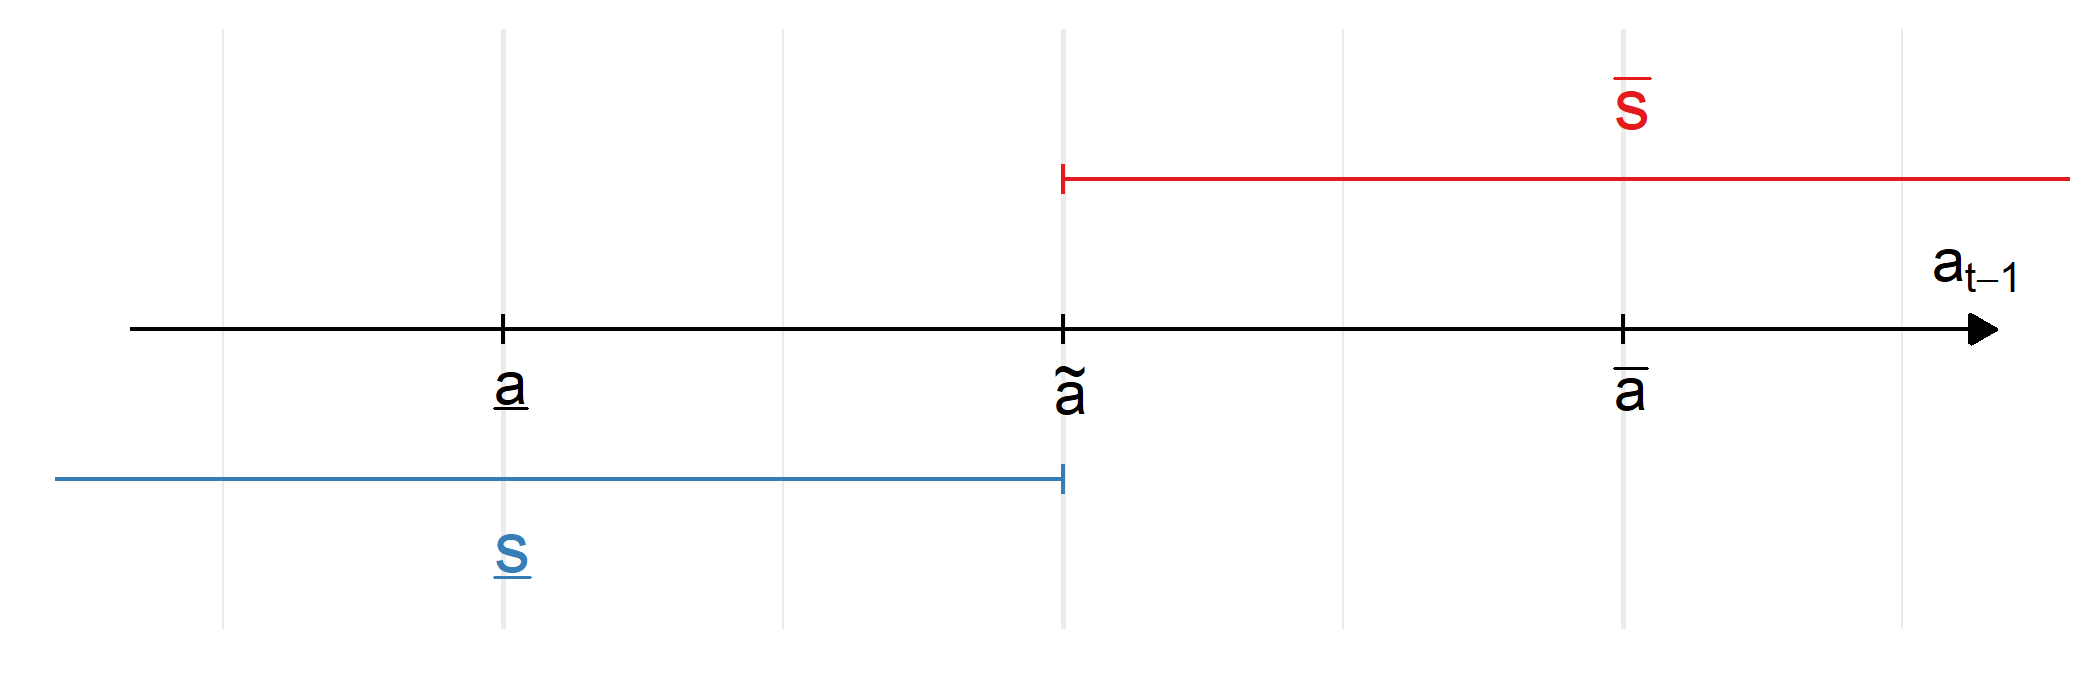
\includegraphics[width=.8\linewidth]{chap3/graphic/theory-choice-a.png}
	\vspace{-3em}
	\justify\singlespacing\footnotesize{\textit{Notes:} This figure presents the indifference value $\widetilde{a}_{t-1}$ which is defined as the threshold value $a$ in $t-1$ such that the agent is indifferent between both groups. In the single-value model, it corresponds to the midpoint value $\widehat{a}$, which is the middle of the distance between the average values in both groups. When the value $a$ in previous period is lower (resp. higher) than the indifference value, the agent prefers to identify with the group $\underline{s}$ (resp. $\overline{s}$).}
\end{figure}
In the single-value model, as long as the value in previous period $a_{t-1}$ is greater (resp. smaller) than the midpoint value $\widehat{a}$, the agent prefers to belong to group $\overline{s}$ (resp. $\underline{s}$). In absence of shocks on her value, the agent converges toward a steady-state value which corresponds to the average value within her group, and the dynamics is given by equation \eqref{chap3-eq:dyn-1val}. What happens when there is a shock?


If an information shock is sufficiently large, the agent identifies with the other group.\footnote{Based on constructivist psychology, a shock on values consists of an event that brings new information to the agent through an experience (\citealt{Levitt2004Transformational}). This latter challenges the agent by questioning her sense of independence, her emotions, her self-awareness, hence, all her perceptions of the meaning of life (i.e. values).} Suppose the agent belongs to the group $\underline{s}$ and she is in her steady state which means that $a_{t-1} = \underline{a}$. There is a shock $\Delta a_{t-1}$ at the end of the period such that her value becomes $a_{t-1}^\prime = a_{t-1} + \Delta a_{t-1}$. Thus, it is straightforward that the agent prefers to keep with her current group $\underline{s}$ as long as the shock does not push $a_{t-1}^\prime$ beyond the threshold---characterized by the indifference value $\widetilde{a}$. Otherwise, the agent prefers to identify with the other group $\overline{s}$. This result leads to Proposition \ref{chap3-prp:shock}. Proof in appendix \ref{chap3-model}.
\begin{proposition}[Shock existence]\label{chap3-prp:shock}
    For any individual, it always exists an information shock such that she prefers to identify with the other group.
\end{proposition}

%%%%% RESULT 1 %%%%%
The single-value model delivers two main results. First, any individual converges to the average value within her group. The length of time to convergence depends on two components: the rate of convergence and the distance with the group-average value. 
On the one hand, the greater is the ratio $\eta_a/\phi_a$, the more costly is the time inconsistency with respect to the group dissonance, hence, the faster the convergence. 
On the other hand, the further the current value is from the group-average value, the slower the convergence.

%%%%% RESULT 2 %%%%%
Second, it is always possible to find a shock such that an individual starts to identify with the other group. The shock requires two conditions to be satisfied: its direction has to be toward the other-group average value and the magnitude has to be sufficiently large. The magnitude depends on the distance between both groups in terms of value and the current value of the individual. The larger is the distance, the greater has to be the shock. When the current value is in a steady state, the magnitude corresponds to the midpoint distance. Otherwise, the closer she is from the midpoint value, the smaller has to be the shock.

\subsection{Two-value model}

We aim to understand the difference in terms of values dynamics when there are two values instead of one. Suppose there are two (motivational types of) values $V_t = (a_t, b_t)\in\mathbb{R}^2$. Consider the same utility function as before but including the second value $b_t$. The maximization program of the agent becomes:
\begin{equation}\label{chap3-eq:maxU-2val}
    \begin{split}
        \max_{a_t, b_t, s_t} U_t(a_t, b_t, s_t) = &-\eta_a\frac{\left[a_t-a_{t-1}\right]^2}{2} -\phi_a\frac{\left[a_t-a^\star(s_t)\right]^2}{2}\\
        &-\eta_b\frac{\left[b_t-b_{t-1}\right]^2}{2} -\phi_b\frac{\left[b_t-b^\star(s_t)\right]^2}{2},
    \end{split}
\end{equation}
where $v^\star(s_t) = \{\underline{v}, \overline{v}\}$ is the average-group value $v\in\{a,b\}$ and $(\eta_a, \phi_a, \eta_b, \phi_b)\in (\mathbb{R}^\star_{+})^4$ are parameters that account for the relative importance of each utility components. 
%
The agent seeks to avoid the same psychological costs as before, namely, time inconsistency and group dissonance, but on two values instead of one. The optimal values are identical to the single-value model, hence, the weighted average between the past value and the average value within the group:
\begin{align*}
    a_t(s_t) =  \frac{\eta_a a_{t-1} + \phi_a a^\star(s_t)}{\eta_a + \phi_a}, \hspace{2em} \text{and} \hspace{2em}%\label{chap3-eq:foc-1val-a}
    b_t(s_t) =  \frac{\eta_b b_{t-1} + \phi_b b^\star(s_t)}{\eta_b + \phi_b}.%\label{chap3-eq:foc-1val-b}
\end{align*}
Thus, the dynamics of values are also identical to equation \eqref{chap3-eq:dyn-1val} and Proposition \ref{chap3-prp:converge} holds. So far, nothing changes with respect to the single-value model although we add one value.

The difference in this setup arises from the inter-dependence between both values. There exist two groups, $\underline{s}$ and $\overline{s}$, in which the average values are respectively $(\underline{a}, \underline{b})$ and $(\overline{a}, \overline{b})$.
Since values are standardized in the population, it implies that $\underline{v}$ and $\overline{v}$ have opposite signs. 
%
We have set the average value $a$ in both groups such that $\overline{a} > 0 > \underline{a}$.
%
Thus, the inter-dependence between values is captured by the sign of $\overline{b}$ (or equivalently by the sign of $\underline{b}$). If $\overline{b}$ is positive, then both values are positively correlated in the population. Otherwise, they are negatively correlated. 

The inter-dependence between values affects the conditions under which the agent prefers to change her group. To illustrate this, suppose the agent belongs to the group $\underline{s}$ and she is in her steady state such that $a_{t-1}=\underline{a}$ and $b_{t-1} = \underline{b}$.
%
There is an information shock on value $a$ at the end of the period, hence, $a_{t-1}^\prime = \underline{a} + \Delta a_{t-1}$. In period $t$, the agent has to choose whether she wants to stay in her group or change for the other group. Her values depend on this choice. If she decides to stay in her current group, her indirect utility is
\begin{equation}\label{chap3-eq:U1under}
    U_t(\underline{s}) = - \gamma_a \left(\Delta a_{t-1}\right)^2.
\end{equation}
Otherwise, she changes her group and gets the following indirect utility:
\begin{equation}\label{chap3-eq:U1over}
    U_t(\overline{s}) = - \gamma_a \big[\overline{a} - \underline{a}-\Delta a_{t-1}\big]^2
    - \gamma_b \big[\overline{b}-\underline{b}\big]^2,
\end{equation}
where $\gamma_b \equiv \frac{\eta_b\phi_b}{2(\eta_b+\phi_b)}>0$. 

The agent decides to change her group \textit{if and only if} the information shock drives her value $a^\prime_{t-1}$ beyond the indifference threshold $\widetilde{a}$, as depicted in figure \ref{chap3-fig:theory-choice-a}. In this example, the indifference value is derived from equations \eqref{chap3-eq:U1under} and \eqref{chap3-eq:U1over} and corresponds to
\begin{equation}\label{chap3-eq:indiff}
    \widetilde{a} = \widehat{a} + \frac{1}{2\gamma}\frac{\big(\overline{b}-\underline{b}\big)^2}{\overline{a}-\underline{a}},
\end{equation}
where $\gamma \equiv \gamma_a/\gamma_b > 0$ and $\overline{a}-\underline{a} > 0$ by definition.
When both values are orthogonal, i.e. $\overline{b}-\underline{b} = 0$, the indifference value corresponds to the one of the single-value model, namely, $\widehat{a}$.

Figure \ref{chap3-fig:theory-shift-a} presents the indifference value as a function of the degree of inter-dependence between values.
\begin{figure}[!tb]
    \centering
    \caption{Indifference value and inter-dependence between values}
    \label{chap3-fig:theory-shift-a}
    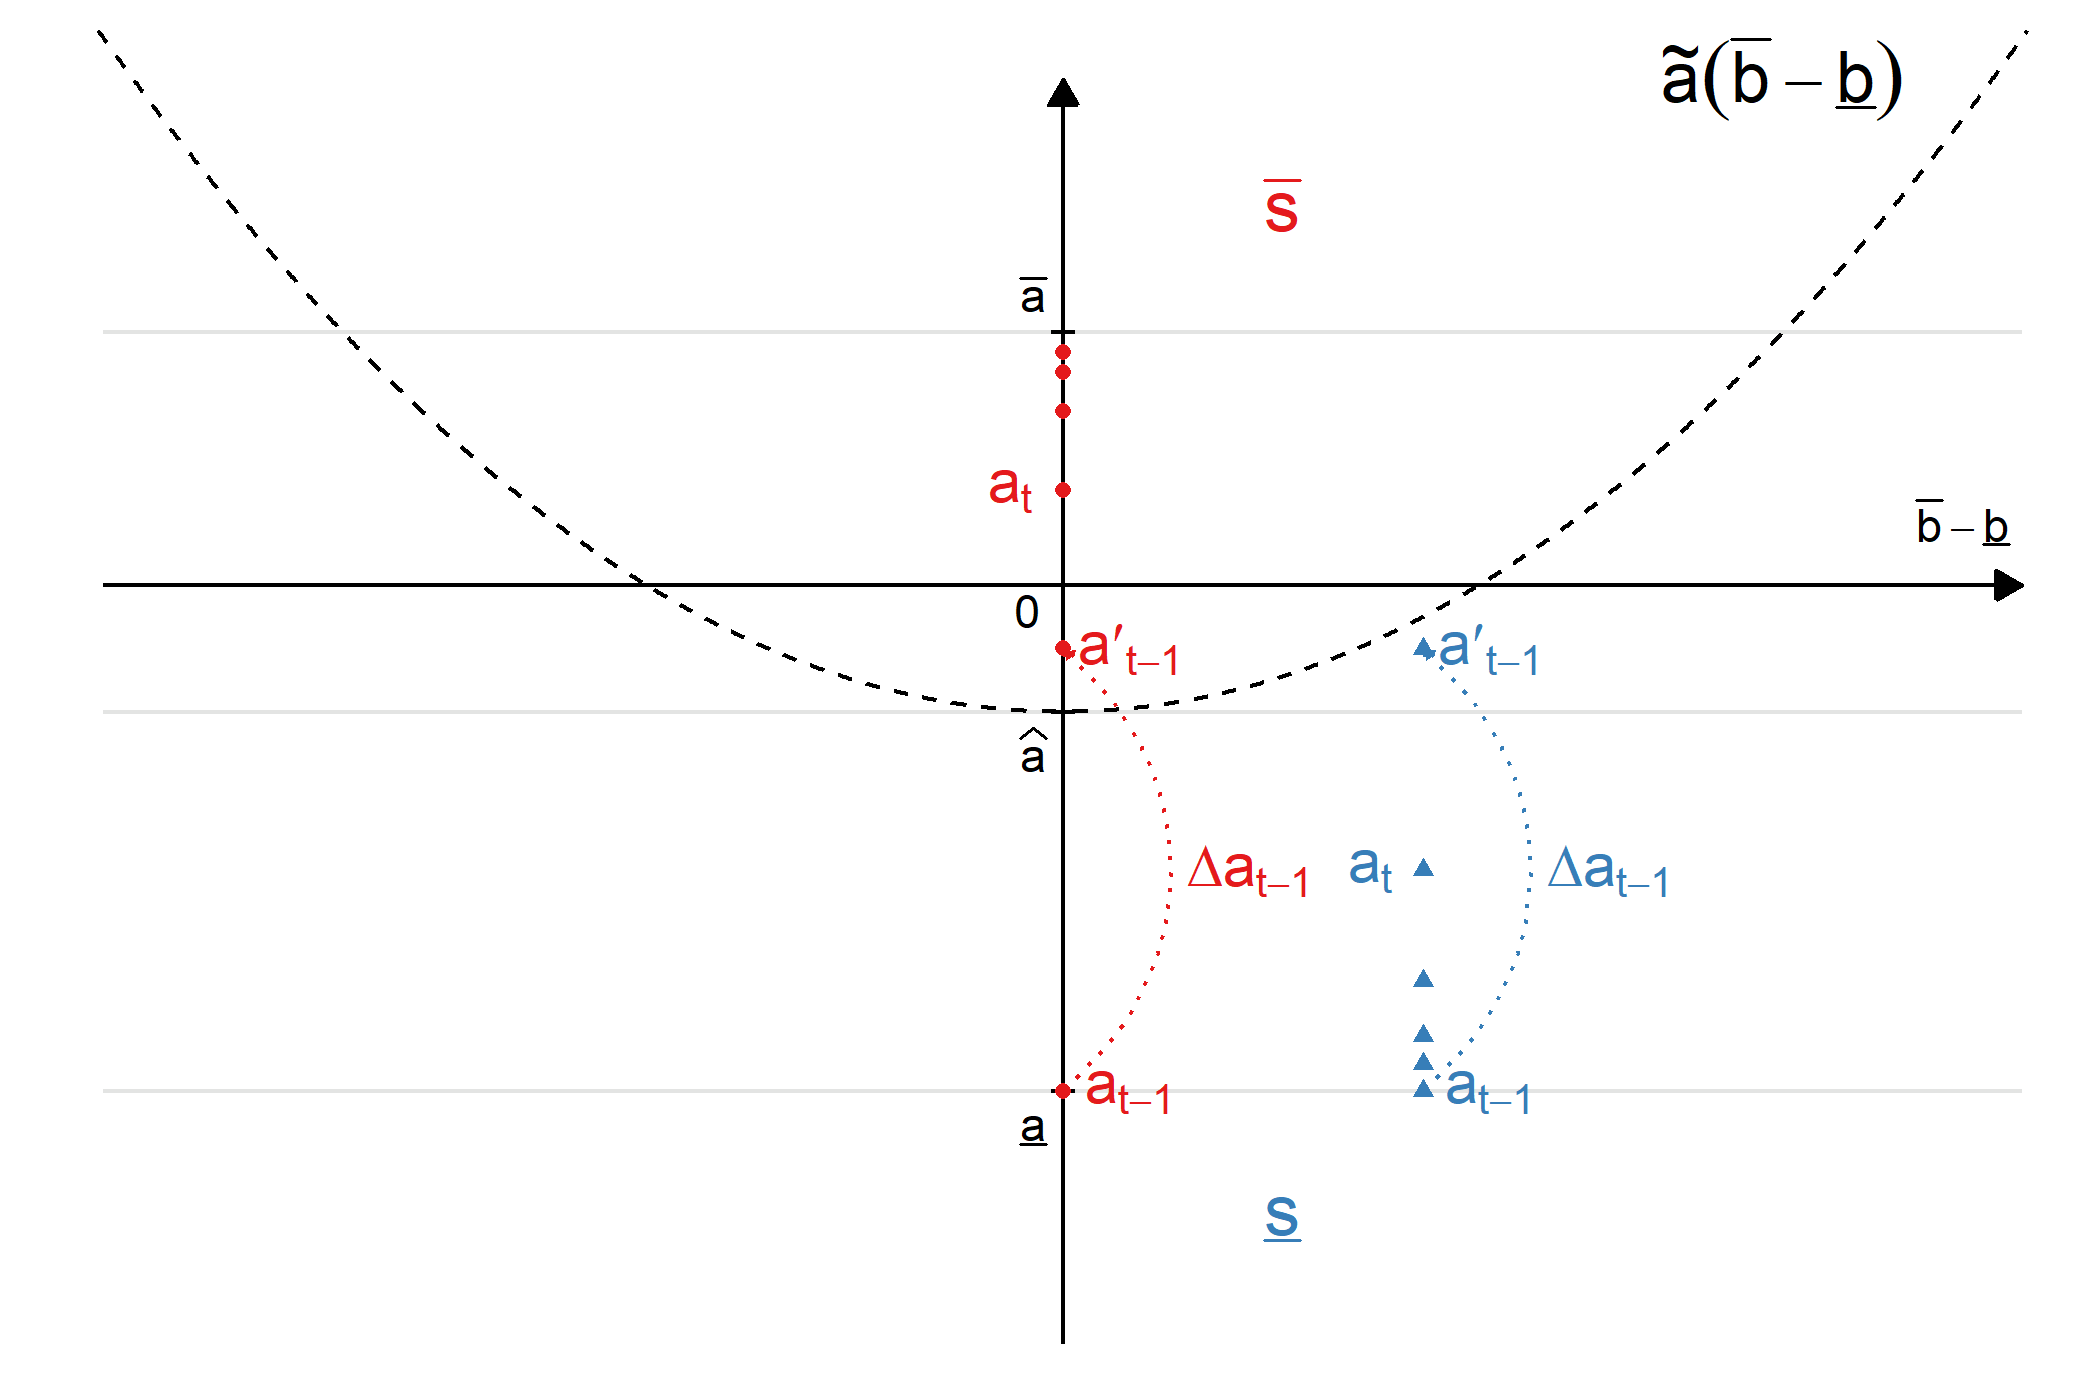
\includegraphics[width=\linewidth]{chap3/graphic/theory-shift-a.png}
	\vspace{-3em}
	\justify\singlespacing\footnotesize{\textit{Notes:} This figure presents the indifference value as a function of the degree of inter-dependence between values. The x-axis corresponds to the gap between both group averages in terms of value $b$. As $\overline{a}-\underline{a} > 0$, it implies that the magnitude of $\overline{b}-\underline{b}$ corresponds to the degree of inter-dependence---values are either positively correlated on the right-hand side of the figure or negatively correlated on the left-hand side.
	The y-axis corresponds to the value $a$. 
	The dash line refers to the indifference value $\widetilde{a}$ and indicates the frontier of indifference between both groups $\overline{s}$ and $\underline{s}$. The dotted curve shows an information shock $\Delta a_{t-1}$ in two different settings, based on the degree of inter-dependence, which lead to different group memberships.}
\end{figure}
The right-hand side of the figure corresponds to cases in which both values are positively correlated, whereas the left-hand side refers to those in which they are negatively correlated. The dashed line represents the indifference value $\widetilde{a}$, which is a function of the distance between both group-average values in $b$, hence, the inter-dependency.

Starting with the area below the dashed curve, any information shock that shifts the value $a$ in this area is not sufficiently large to change the agent's group membership. Thus, agent's value $a$ converges back to its steady-state value $\underline{a}$, and value $b$ has not changed meanwhile.
Conversely, any information shock that brings the value $a$ above the indifference value implies a change in the group membership of the agent. As the agent identifies with the other group, she changes both of her values. In the long run, she converges toward the average values of the other group, namely, $\overline{a}$ and $\overline{b}$. Although the value $b$ was not initially affected by the information shock, the agent has changed her value $b$ to be consistent with the values in her new group. Thus, the two-value model provides a theoretical framework for the existence of spillover effects that is based on group consistency.

Proposition \ref{chap3-prp:shock} holds when there is an additional inter-dependent value, meaning that it is always possible to find a shock sufficiently large such that she prefers to identify with the other group.
Nonetheless, it leads to Proposition \ref{chap3-prp:relevant}.%
\begin{proposition}[Value relevance]\label{chap3-prp:relevant}
    If a value poorly discriminates groups with respect to the other, then this value is less relevant in the individual's choice of group membership.
\end{proposition}%
% % How?
When the gap between groups in terms of value $b$ is large in absolute terms, i.e. $\left|\overline{b}-\underline{b}\right| \gg \overline{a}-\underline{a}$, it indicates that the polarization between both groups in terms of $b$ is important with respect to the one in terms of $a$. Thus, the value $a$ is less relevant for values dynamics as only a very large shock on $a$ can make the agent identify with the other group. This is due to the fact that the group dissonance with respect to $b$ generates a psychological cost that can hardly be offset by any other consideration than keeping up with the current group---except with a large information shock.

\subsection{Predictions of the model}

The theoretical framework provides several predictions about the dynamics of values. 
Proposition \ref{chap3-prp:converge} indicates that, in absence of information shocks, any individual converges in values toward the values of her group.
Proposition \ref{chap3-prp:shock} predicts that, for any individual, it is always possible to find an information shock such that the agent identifies with the other group. The corollary implies that there exist small shocks for which the individual is only affected in the short run as she does not change group.
Both previous predictions hold when the individual is characterized by two values that are correlated across groups, hence, inter-dependent.
Proposition \ref{chap3-prp:relevant} predicts that values that discriminate the most between groups are those that are the most relevant in the choice of the individual about group membership.

The theoretical framework also raises an important issue about considering only one value at a time. The consistency trade-off in individual's group membership depends on the degree of inter-dependence between values across groups. As a result, neglecting this inter-dependence leads to underestimating the role of the group in values dynamics. Thus, the greater the correlation of values across groups, the larger has the shock to be for the agent to change group.

Lastly, Proposition \ref{chap3-prp:spillover} gives the main prediction of the theoretical framework about the existence of spillover effects across values.
\begin{proposition}[Spillover effect]\label{chap3-prp:spillover}
    If two values are inter-dependent, then an information shock on one value can trigger a spillover effect on the other value.
\end{proposition}
When an information shock---due to a life-changing event---on one value is sufficiently large, the individual identifies with another group, thus, she changes both of her values. Although the other value was not initially affected, the life-changing event has also changed this value indirectly through the spillover effect. I turn to empirical analysis in order to test the existence of spillover effects among values.
    
    \section{Data} \label{chap3-data}
    \subsection{Sample}

% What data ?
I use two mature British cohort studies: the National Child Development Study (NCDS58) is a cohort of individuals born during the same week in March 1958; the British Cohort Study (BCS70) is composed of those born during the same week in April 1970. 
% Where are they born ?
Cohort members were born in England, Scotland and Wales.

% Interviews
Both cohorts participated in several interviews at different ages.
% Figure
Figure \ref{chap3-fig:data-itw-values} presents the ages at which cohort members may have been interviewed and the corresponding years.
\begin{figure}[!tb]
    \centering
    \caption{Timing of interviews}
    \label{chap3-fig:data-itw-values}
    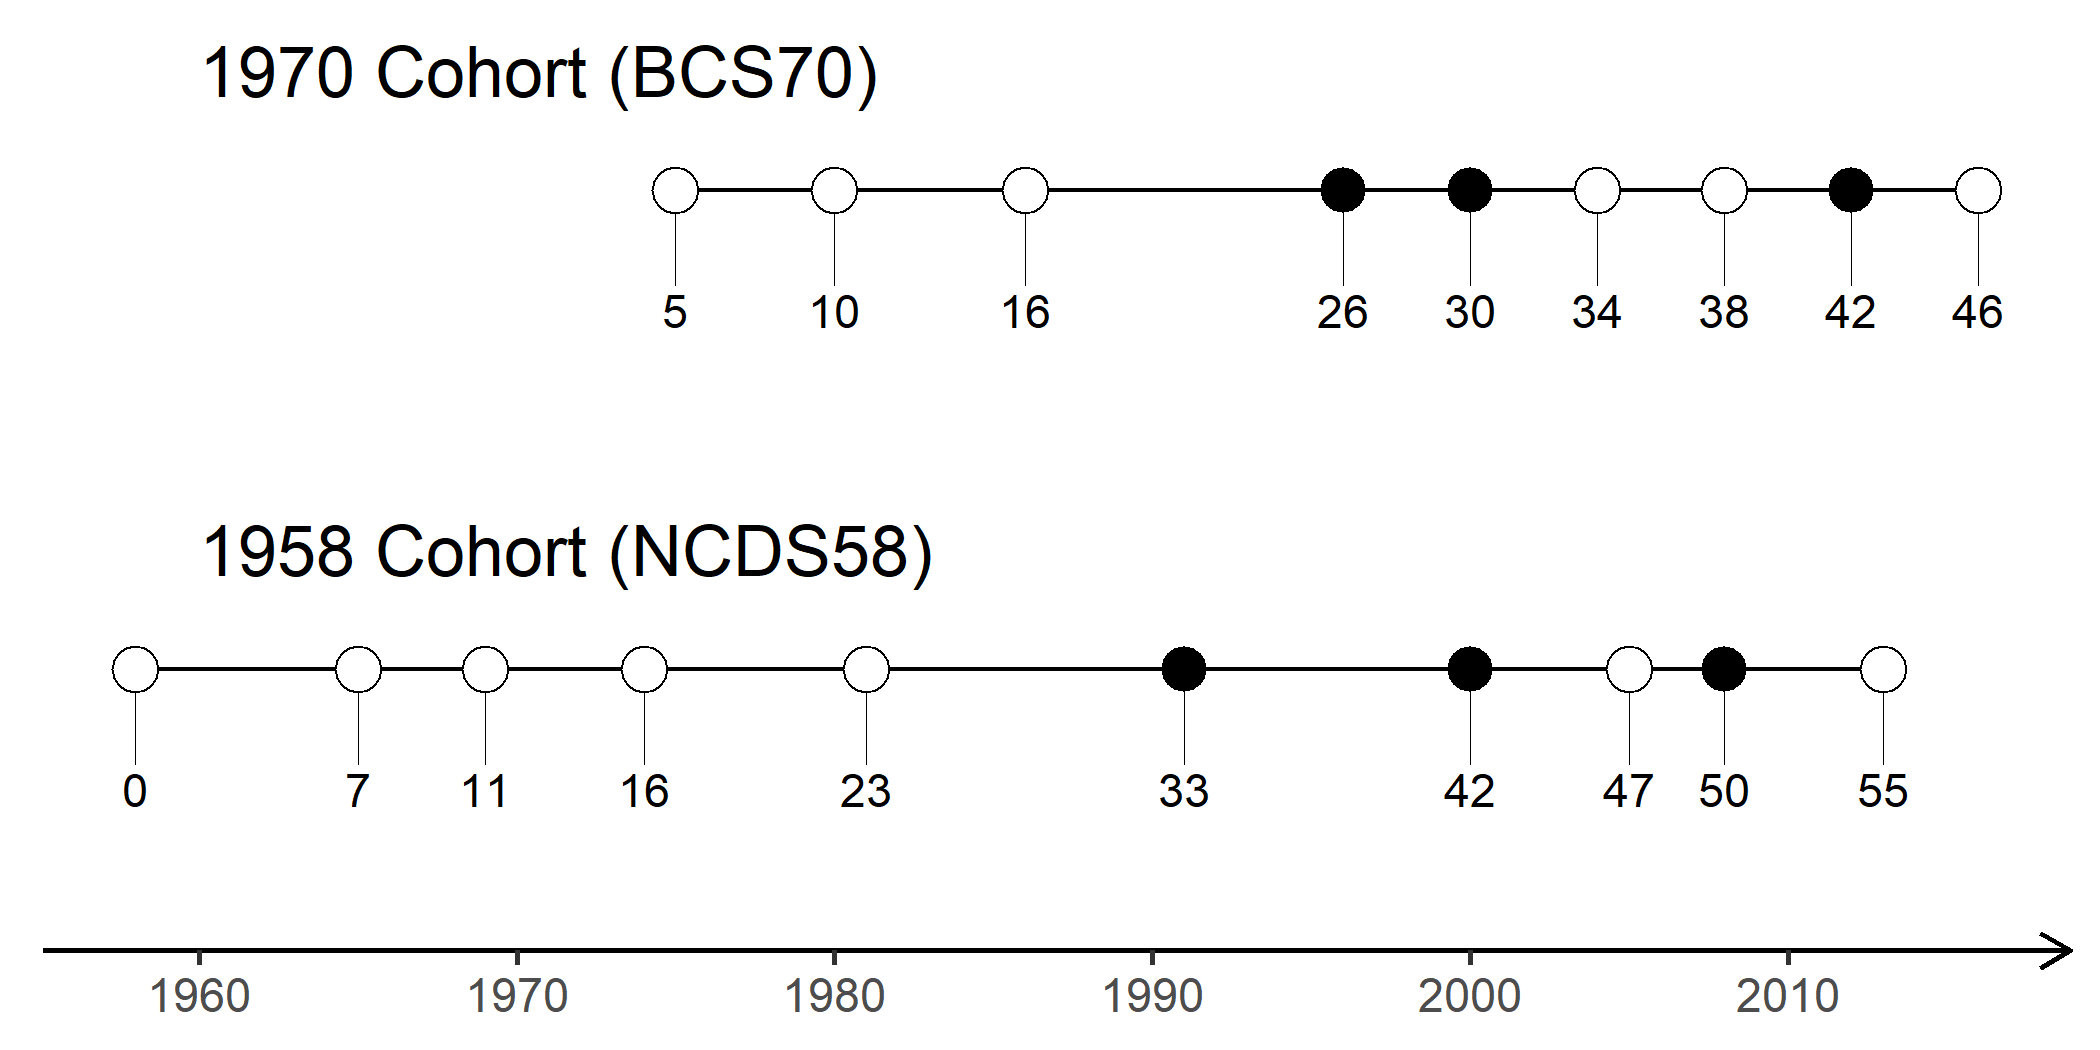
\includegraphics[width=\linewidth]{chap3/graphic/data-itw-values.png}
    \hrulefill
	\vspace{-3em}
	\justify\singlespacing\footnotesize{\textit{Notes:} This figure presents the timing of interviews for the NCDS58 and BCS70 cohorts. Circles correspond to interviews and numbers under them indicate the age of cohort members during this interview. Full circles correspond to interviews for which attitudes can be derived. The horizontal arrow at the bottom of the figure represents the years.}
\end{figure}
% Attitudes available
The full circles on the figure indicate interviews from which values can be derived, thus I will focus on those years for the remaining of the paper.
% Periods definition
I define four periods according to the decade in which individuals belong, i.e. their twenties, thirties, forties, or fifties.
% BCS periods
For the BCS70 cohort, I refer to period 1 for the interview at the age of 26, to period 2 for the one at 30, and to period 3 for the one at 42.
% NCDS periods
For the NCDS58 cohort, periods start at period 2 for the interview at the age of 33, then period 3 corresponds to the one at 42, and period 4 refers to the one at 50.

% Attrition ?
One of the main issues with cohort studies is attrition. 
% Either missing interviews OR lose them
Cohort members do not participate at every interview and therefore some individuals are either missing at some interviews or lost definitely at some point.
%
Table \ref{chap3-tab:data-resp} presents the responses rates by periods of interest.
% Table to show attrition
\begin{table}[!tb]
    \centering
    \caption{Number of individuals and response rates by periods.}
    \label{chap3-tab:data-resp}
    \begin{threeparttable}
        \setlength{\tabcolsep}{15pt}
        
\begin{tabular}{lrr}
\toprule
  & \multicolumn{1}{c}{BCS} & \multicolumn{1}{c}{NCDS}\\
\midrule
Initial & 19,006 (100\%) & 17,885 (100\%)\\
\midrule
Period 1 & 9,003 (47.4\%) & \\
Period 2 & 11,261 (59.2\%) & 11,469 (64.1\%)\\
Period 3 & 9,841 (51.8\%) & 11,419 (63.8\%)\\
Period 4 &  & 9,790 (54.7\%)\\
\midrule
All & 6,115 (32.2\%) & 8,107 (45.3\%)\\
\bottomrule
\end{tabular}

        \begin{tablenotes}[flushleft]
            \footnotesize{\item \textit{Notes}: Response rates between parentheses. The last row corresponds to individuals who have been interviewed at all periods.}
        \end{tablenotes}
    \end{threeparttable}
\end{table}
%
The second-period interview is the one with the greater response rate, i.e. 64.1\% for the NCDS58 cohort and 59.2\% for the BCS70 one. This latter interview, when BCS70 cohort members are 30, has been conducted at the same time as the third-period interview for the NCDS58 cohort, when they are 42, so in the year 2000. Thus, they share the same set of variables.

\subsection{Motivational types of values}

% Attitudes from statements
I derive values from individuals' answers to statements about their attitudes.\footnote{In social psychology, an attitude toward an object---such as a statement---corresponds to emotions, beliefs, and behaviors toward this particular object.} At each interview, cohort members answer to statements using a 5-level scale (strongly disagree / disagree / neither agree nor disagree / agree / strongly agree). I attribute them a score for each statement between -2 and 2 according to the answer.

% Group statement by categories
These statements cover several attitudes and can be grouped into categories (in alphabetical order): Anti-Racism (AR), Authority (A), Children (C), Environment (E), Inequality Aversion (IA), Information Technology (IT), Learning (L), Morale (MOR), Political Cynicism (PC), Work-Ethic (WE), and Working Mother (WM). 
The full list of statements are reported in appendix \ref{chap3-statement}. Some examples of statements are the following:
\begin{table}[!h]
    % \footnotesize
    \renewcommand*{\arraystretch}{1.5}
	\begin{tabular}{rl}
    (A2)    & \textit{For some crimes the death penalty is the most appropriate sentence};\\
    (MOR3)  & \textit{Couples who have children should not separate};\\
    (PC1)   & \textit{None of the political parties would do anything to benefit me};\\
    (WE1)   & \textit{Having almost any job is better than being unemployed}.
    \end{tabular}
\end{table}

% Compute the average score
\noindent I compute the average score within each attitude category for each individual at each period. Thus, each individual has a score for each attitude in each period. Then, I standardize each attitude score at the cohort and period level. Thus, each individual belongs to a cohort and has, for each period, a standardized score for each attitude that is relative to her cohort in a given period.

%
Nonetheless, the number of available statements depends on the cohort and the period. Table \ref{chap3-tab:data-available-short} summarizes the number of available statements at each interview.
\begin{table}[!tb]
    \centering
    \caption{Number of available statements at each interview}
    \label{chap3-tab:data-available-short}
    \begin{threeparttable}
        \setlength{\tabcolsep}{12pt}
        \begin{tabular}{lrrrrrr}
\toprule
\multicolumn{1}{c}{} & \multicolumn{3}{c}{BCS70} & \multicolumn{3}{c}{NCDS58} \\
\cmidrule(l{3pt}r{3pt}){2-4} \cmidrule(l{3pt}r{3pt}){5-7}
Attitude & 26 & 30 & 42 & 33 & 42 & 50\\
\midrule
Authority & 4 & 6 & 3 & 6 & 6 & 3\\
Anti-Racism &  & 5 & 2 & 5 & 5 & 3\\
Children &  & 4 & 2 & 2 & 4 & \\
Environment &  & 3 & 2 & 3 & 3 & 3\\
Inequality Aversion & 1 & 7 & 5 & 7 & 7 & 3\\
Info. Techno. &  & 4 &  &  & 4 & \\
Learning &  & 4 &  &  & 4 & \\
Morale & 3 & 6 & 3 & 6 & 6 & 3\\
Political Cynicism & 3 & 3 & 3 & 3 & 3 & 3\\
Work Ethic & 2 & 3 & 3 & 3 & 3 & 3\\
Working Mother &  & 5 & 2 &  & 5 & \\
\bottomrule
\end{tabular}
        \begin{tablenotes}[flushleft]
            \footnotesize{\item \textit{Notes}: This table presents the number of available statements in each attitudes at each age for the NCDS58 and BCS70 cohorts. Details on statements are reported in the appendix, see tables \ref{chap3-tab:statement-split-1}, \ref{chap3-tab:statement-split-2} and \ref{chap3-tab:statement-split-3} in appendix \ref{chap3-statement}.}
        \end{tablenotes}
        \end{threeparttable}
\end{table}
%
Thus, interviews do not necessarily share the same set of statements, except when the BCS70 cohort is 30 and the NCDS58 cohort is 42 because interviews were performed using the same questionnaires.

I derive motivational types of values from these attitude scores. I focus on the five attitudes that are available in all interviews in order to have the same baseline for each period of both cohorts. These attitudes are Authority (A), Inequality Aversion (IA), Morale (MOR), Political Cynicism (PC), and Work Ethic (WE).

%
I use a Principal Component Analysis (PCA) to transform the 5-dimension attitudes into the two-dimension motivational types of values. PCA increases the interpretability of vectors while minimizing the information loss. By focusing on the two first components, which are orthogonal by the construction of the PCA, I can interpret them as the two main values that discriminate and, therefore, characterize individuals in their attitudes. 

The other principal components act as residuals to some extent. Although they might be incorporated into the analysis, Proposition \ref{chap3-prp:relevant} states that a value needs to be sufficiently discriminatory between groups in order to be relevant in the group membership decision. The two first principal components capture more than 50\% of the explained variance in attitudes, which makes the discriminatory power of the other principal components less relevant.
% \footnote{PCA allows to determine values by summarizing attitudes through dimension reduction which reduces the noise in attitudes, hence, this noise is relegated to the unused components that explain the smaller part of the variance and are not relevant.} Therefore, I focus on the two first components.

%
I perform PCA at the cohort and period level. Figure \ref{chap3-fig:data-pca-v5} presents the eigenvectors of the two first principal components.
\begin{figure}[!tb]
    \centering
    \caption{Eigenvectors of the two first principal components}
    \label{chap3-fig:data-pca-v5}
    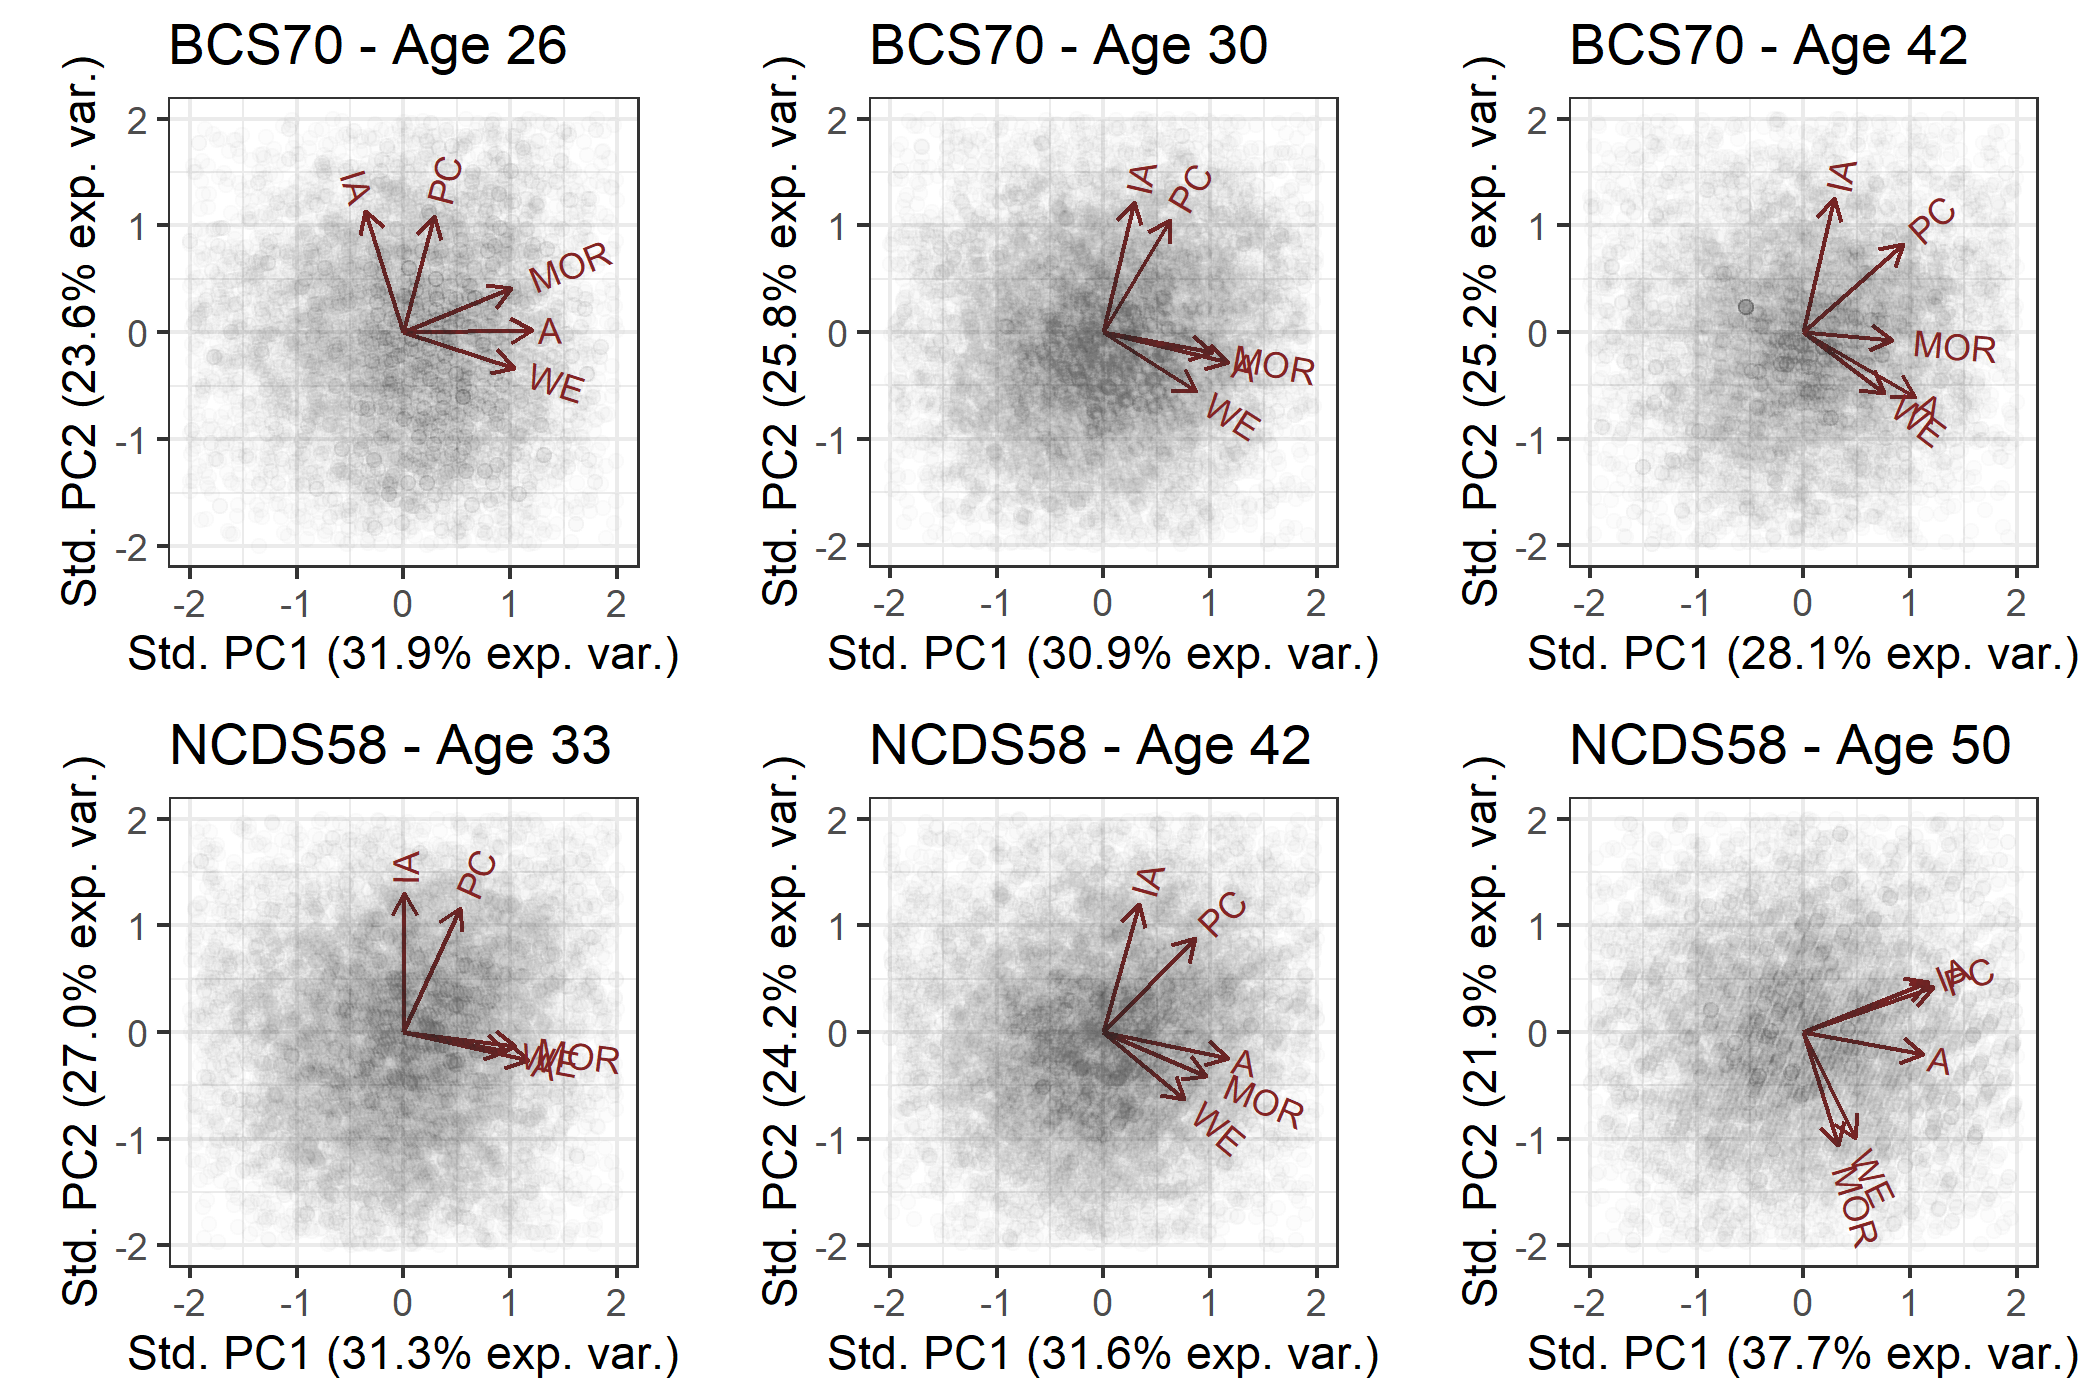
\includegraphics[width=\linewidth]{chap3/graphic/pca-v5.png}
    \hrulefill
	\vspace{-3em}
	\justify\singlespacing\footnotesize{\textit{Notes:} This figure presents the eigenvectors of the two first principal components. Details on the eigenvectors are available in tables \ref{chap3-tab:pca-v5-BCS70} and \ref{chap3-tab:pca-v5-NCDS58}, respectively for the BCS70 and NCDS58 cohorts. Attitudes are Authority (A), Inequality Aversion (IA), Morale (MOR), Political Cynicism (PC) and Work Ethic (WE).}
\end{figure}
Links between attitudes are fairly stable across cohorts and periods. These principal components explain more than 50\% of the variance in attitudes. I interpret both of them as the two-dimensional structure of universal motivational types of values, as introduced by \citet{Schwartz1992Universals, Schwartz2012Overview}---see figure \ref{chap3-fig:schwartz} in the appendix.

% PC1
Focusing on the first principal component (PC1), the x-axis directions of vectors highlight attitudes that characterize \textit{conservatism} which is the preference for stability, security, tradition, and conformity. In the data, they reflect a taste for attitudes about Authority, Morale, and Work Ethic. Thus, the dimension that discriminates the most between individuals is \textit{conservatism} (versus \textit{progressivism}).
% PC2
The second principal component (PC2) is orthogonal to the previous dimension of values at the cohort-period level. Focusing on the y-axis directions of vectors, they indicate attitudes that characterize \textit{collectivism}. This motivational type of values refers to the care and concern about others, reflecting universalism and benevolence. In the data, this value is associated with attitudes toward Political Cynicism and aversion for Inequality and Work Ethic. Therefore, the second discriminatory dimension between individuals is \textit{collectivism} (versus \textit{individualism}).\footnote{In the terms of \citet{Schwartz1992Universals}, both dimensions are respectively named conservation (versus openness-to-change) and self-transcendence (versus self-enhancement).}

% Projection
I make a projection of both principal components for all individuals at each period.  Thus, each cohort member has a Conservatism score ($Cons$) and a Collectivism score ($Coll$) at each period. By construction, both scores are standardized at the cohort-period level and \textit{orthogonal}. Thus, the values are not inter-dependent \textit{per se}. The inter-dependency arises with socio-economic characteristics---such as gender, education, etc.---once they are introduced as control variables. These covariates capture several dimensions of groups to which individuals identify, hence, it creates inter-dependency between values as they are correlated among groups.

\subsection{Groups mapping using political vote}

In my theoretical framework, the agent belongs to a group and the spillover effect occurs once the agent identifies with another group. Defining groups is therefore crucial to understand spillover effects as we expect individuals to change groups along with their values. So far, a group can be interpreted as composed of peers with whom the agent identifies in terms of values. One can think about those peers as close people such as relatives, neighbors, or colleagues; since we tend to share values with them. Nonetheless, most of the time, individuals cannot freely break off all ties with those latter as there may be direct costs. These direct costs thwart the identification of changes in group membership as they introduce noise through bonds. Thus, I cannot rely on peers to define groups.

An alternative proxy for groups is political vote. There is no direct cost in voting for one party or another at the general election, conditional on voting. In addition, political parties reflect part of individuals' values in the sense that the agent decides to identify with one party with respect to others when voting.

Figure \ref{chap3-fig:vote-v5} presents a mapping of values of the average voters for each main political party at the closest general election (GE); see table \ref{chap3-tab:data-vote} in appendix \ref{chap3-details} for the shares of vote in both cohorts.
\begin{figure}[!tb]
    \centering
    \caption{Average values according to political vote}
    \label{chap3-fig:vote-v5}
    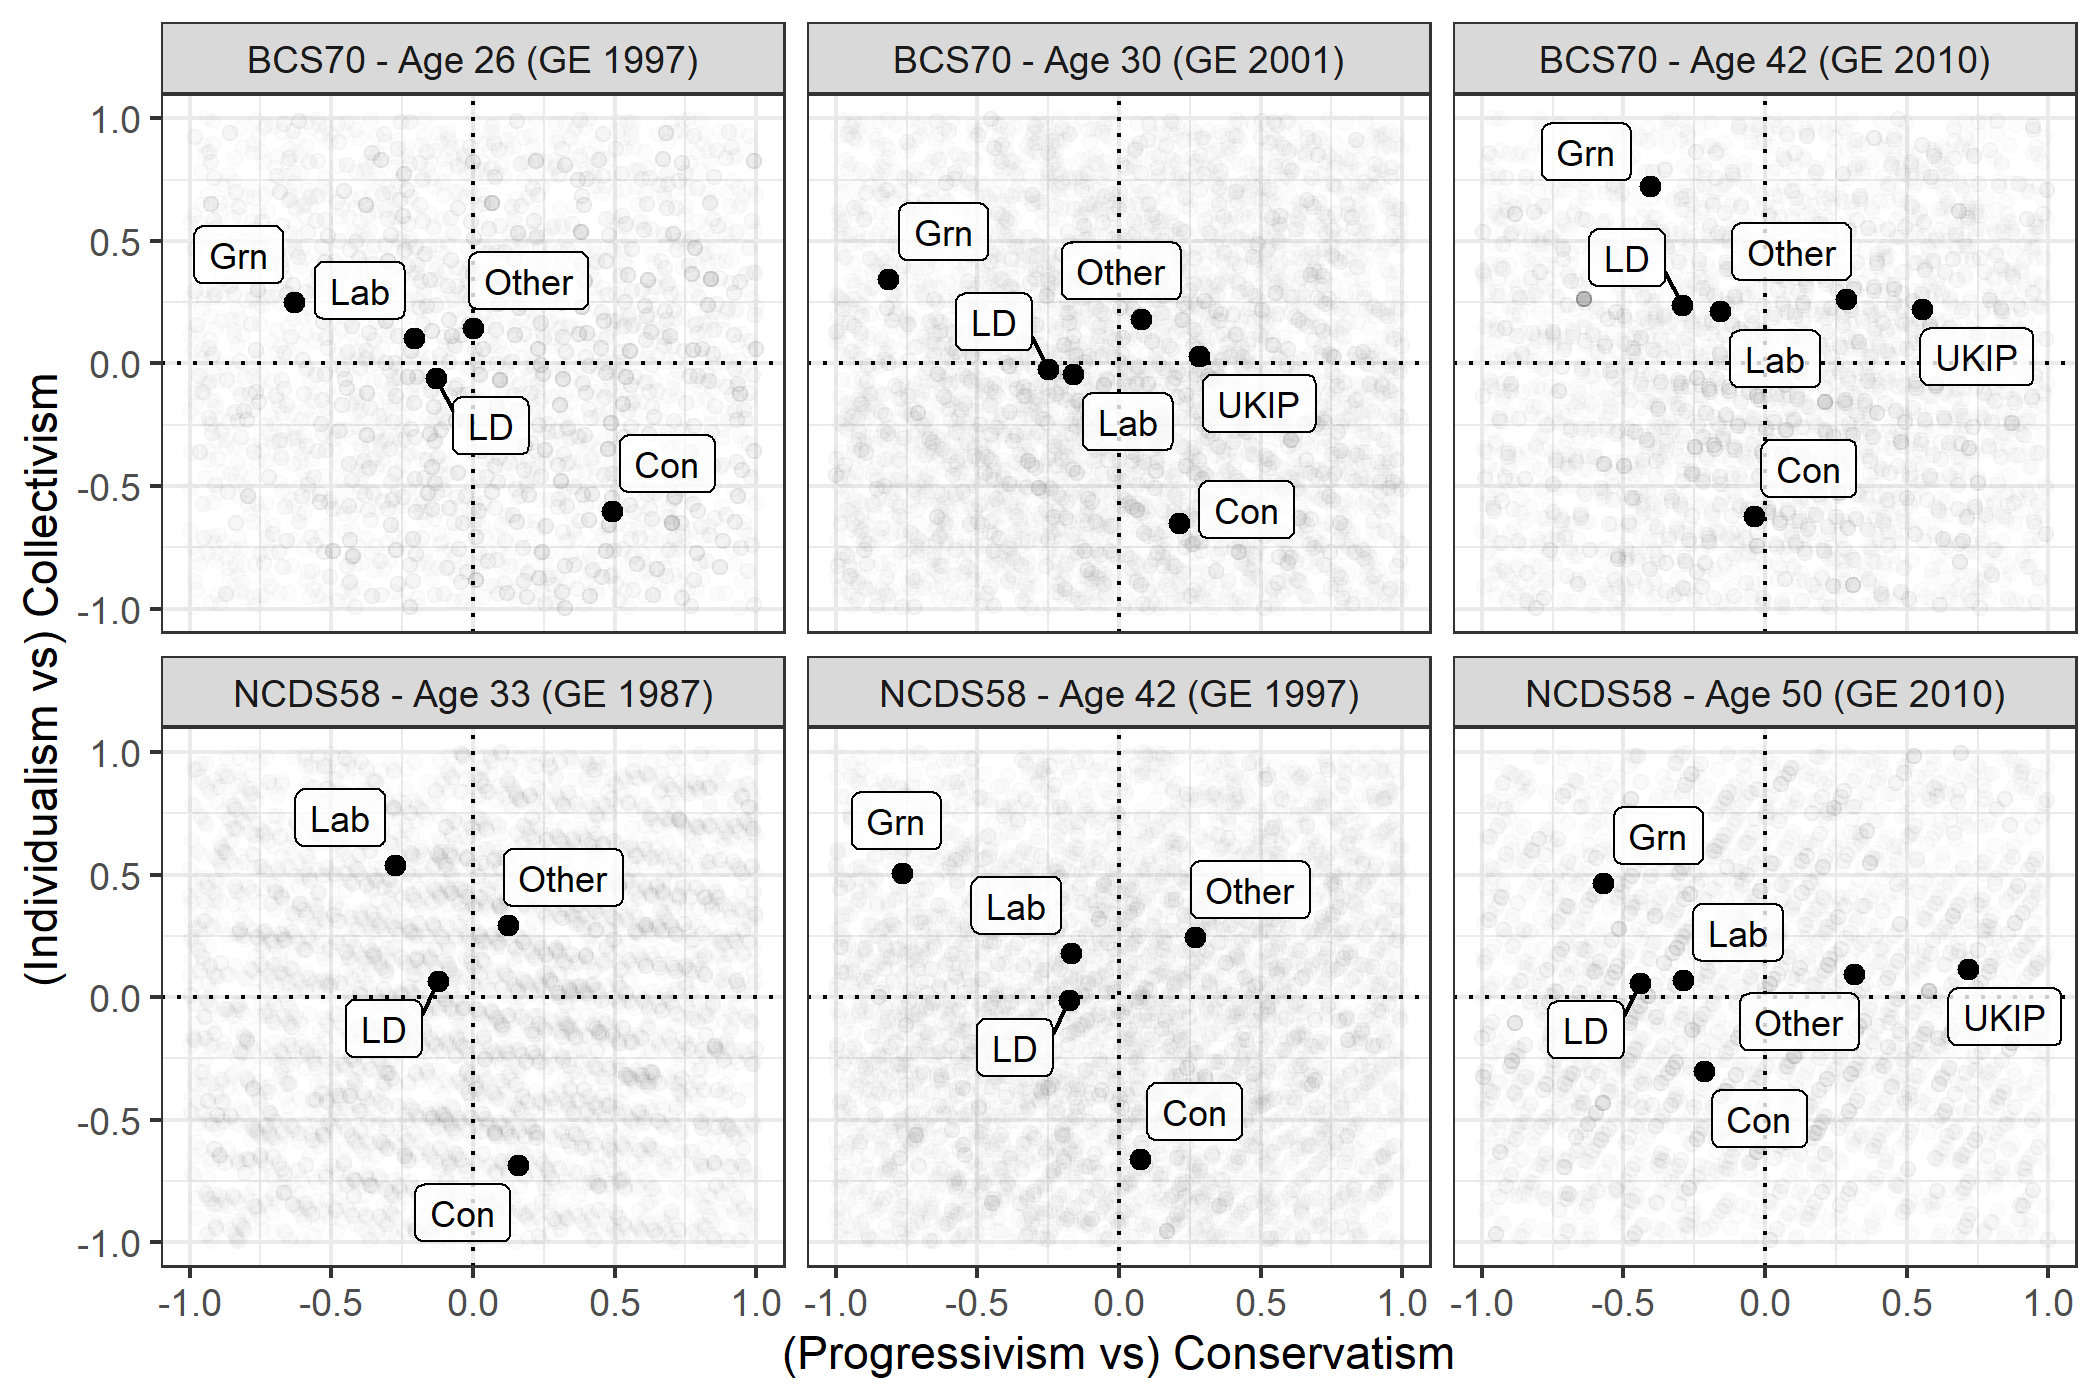
\includegraphics[width=\linewidth]{chap3/graphic/vote-v5.png}
    \hrulefill
	\vspace{-3em}
	\justify\singlespacing\footnotesize{\textit{Notes:} This figure presents the mapping of average scores in conservatism and collectivism according to political voting in General Elections (GE). Political parties are (in alphabetical order): Conservative (Con), Green (Grn), Labour (Lab), Liberal Democrat (LD), and UK Independence Party (UKIP). Other encompasses all other parties, blank votes and abstention.}
\end{figure}
% 1987 GE
The bottom-left panel represents the mapping of values in the 1987 General Election for which only the NCDS58 cohort voted at age 33. Positioning of the two main UK political parties is consistent: Labour (Lab) voters are progressive and collectivist, whereas Conservative (Con) voters are conservative and individualist. The Liberal Democrats (LD) provides an in-between the Labour and Conservative parties.\footnote{Note that the Liberal Democrats party only appeared in 1988 as the merge of the SDP–Liberal Alliance that was running into general elections in 1987. For the ease of exposition, I refer to the SDP–Liberal Alliance in 1987 as the Liberal Democrats.}
Other encompasses all other parties, blank votes, and abstention.
% 1997 GE
The top-left and bottom-mid panels correspond to the 1997 General Election. The Green party (Grn) emerged and attracted voters with progressive and collective values. The overall structure of values and voting is stable across cohorts.
% 2001 GE
The top-mid panel shows the rise of the far-right party UKIP for the 2001 General Election. As the formation of political parties is endogenous, it is unsurprising that it emerged in an area where there was no political supply.
% 2010 GE
Both right panels depict the political mapping for the 2010 general election. The average political voters of the BCS70 cohort are more spread along the collectivism axis, while those in the older cohort are rather spread on the conservatism axis.

Positionings of political parties relative to each other are consistent---over time and across cohorts---on the two-dimensional values' space. Thus, I consider the political vote of individuals as a proxy of their group membership in the remaining of the empirical analysis. This proxy helps understand how individuals start to identify with other groups after life-changing events.

\subsection{Life-changing events}

We are interested in life events that generate information shocks on conservatism ($Cons$) or collectivism ($Coll$) in order to show whether there exist spillover effects or not. The type of life events that I have to consider to test this hypothesis requires two properties: \textit{exogeneity} and \textit{non-reversibility}.
On the one hand, the life event has to be exogenous so that values in the previous period do not influence the likelihood that the life event occurs. 
On the other hand, the life event has to be non-reversible. Otherwise, the probability to reverse the event is likely to be endogenous which would bias the estimate of individual's values at the time of interviews.\footnote{Note that life events that provide temporary shocks are also interesting to study. Especially if a temporary shock leads to a change in groups. In the absence of reverse shock, both---time and group---consistencies would prevent the individual to come back to her previous group's values. Thus, a sufficiently large temporary shock can have long-run consequences on individuals' values.}

In this regard, I focus on two life events that satisfy both properties, namely, \textit{to have ever had cancer} and \textit{to have a girl as first child conditional on having a baby}.
%
The former life event is exogenous in the sense that values, such as conservation and collectivism, do not affect the probability to have cancer---excluding individuals with lung cancer. It is also non-reversible as I compare individuals who have \textit{ever} had cancer with respect to those who never had one. I set the focus on the information shock related to the fact that people have known they have cancer, not on the illness \textit{per se} as someone might have one without knowing it.
Note that for the older cohort at age 50, there may be a bias when considering the effect of this life event on values. As people turn 50, they expect that their health condition will deteriorate in the coming years, thus, they may anticipate such a life event and change their values beforehand. This potential mechanism would bias my estimate toward zero as the control group---those who did not get cancer yet---anticipate and shift their values in the same direction as those who have been treated. Therefore, for this cohort at that age, my approach is likely to provide a lower bound estimate of the effect of having ever had cancer on values.

For the latter life event, I consider a sub-sample that only contains individuals who have at least one baby, hence, I compare those who had a girl as a first child with those who got a boy.
Thus, the life event is exogenous to values because the probabilities of child's sex at birth are fifty-fifty, considering that sex‐selective abortion is very rare in the UK.\footnote{
\citet{Dubuc2007Increase} argue that sex-selective abortion occurs among mothers born in India and living in Britain. They show that sex ratios at birth have always been one point lower for Asian groups in England and Wales before 1990. Although this issue raises several social and economic concerns, it does not statistically affect my results as they represent a minority in the data.} Once the baby is born, the life event is non-reversible because it has occurred and remains forever.
I do not also consider adopted children because the sex may be decided by parents and therefore linked to values and preferences (\citealt{Dahl2008Demand}). I also exclude stillborn babies because the socialization of parents with the baby does not occur.\footnote{Note that this tragic life event could also be considered as a potential life event that would deeply affect values.}

%
I only focus on the first child as fertility decisions for following children might be linked to the sex of the eldest child and values, e.g. a preference for diversity in children's birth sex. Moreover, some parents may have a boy as their first child and a girl thereafter. Some changes in values may be specific to having a girl even though she is not the first baby. Thus, this is likely to produce a lower-bound estimate and also to reduce the statistical power of effects of this life event on values.

Lastly, I study the role of unemployment on values as it is a sizeable information shock in individuals' life. Nonetheless, I cannot use it as a life event to show the existence of spillover effects among values because it does not satisfy both properties. First, individuals change their activity status quite often and, therefore, the effect of unemployment on values is all the time affected by these changes in status. Second, the likelihood to be unemployed is clearly endogenous to values. For instance, one might argue that individuals with high work ethic, hence high conservatism and high individualism, have a lower probability to be unemployed as they are less likely to quit their job with respect to people with low work ethic.

\subsection{Variables and summary statistics}

%%%%% LIFE EVENT VARIABLES %%%%%
For life events, I focus on three of them: to have had a girl as a first child, to have ever had cancer, and to have ever been unemployed. $GirlFirst$ is a dummy variable that equals one if the sex of the first child is female, and zero if it is a male. $GotCancer$ is also a dummy variable that equals one if the individual has ever had cancer by the time of the interview. $BeenUnemp$ is a dummy variable that equals one if the individual has ever been unemployed at least one month by the time of the interview. 
% Activity history
Activity status is derived from the full activity histories to the nearest month since cohort members are 16 years old. These data are available for all cohort members until the last interview they have participated in. When individuals were missing in previous interviews, interviewers asked them about their activities during the period until then.

%%%%% SOCIO-ECONOMIC CHARACTERISTICS %%%%%
I consider several socio-economic characteristics as control variables that will introduce the inter-dependency between values. Among them, I use the sex at birth of cohort members and their level of education based on the highest academic qualification they obtained. $Female$ is a dummy variable that equals one if the cohort member is born as a female. I regroup education levels into three categories that characterize primary, secondary, and tertiary education levels ($Educ$). 

%%%%% SUMMARY STATISTICS %%%%%
Table \ref{chap3-tab:data-statdesc} presents the descriptive statistics for the NCDS58 and BCS70 cohorts. Both cohorts contain respectively 30,552 and 27,906 observations. Period variables corresponds to dummy variables to determine the decade in which individuals are.
\begin{table}[!tb]
    \centering
    \caption{Summary statistics}
    \label{chap3-tab:data-statdesc}
    \begin{threeparttable}
        \setlength{\tabcolsep}{5pt}
        
\begin{tabular}{lrrrrrrrrrr}
\toprule
\multicolumn{1}{c}{} & \multicolumn{5}{c}{NCDS58 - N = 30,552} & \multicolumn{5}{c}{BCS70 - N = 27,906} \\
\cmidrule(l{3pt}r{3pt}){2-6} \cmidrule(l{3pt}r{3pt}){7-11}
Variable & Mean & SD & Min & Max & NA & Mean & SD & Min & Max & NA\\
\midrule
Period 1 - Twenties &  &  &  &  &  & 0.31 & 0.46 & 0 & 1 & 0\\
Period 2 - Thirties & 0.35 & 0.48 & 0 & 1 & 0 & 0.40 & 0.49 & 0 & 1 & 0\\
Period 3 - Forties & 0.37 & 0.48 & 0 & 1 & 0 & 0.29 & 0.45 & 0 & 1 & 0\\
Period 4 - Fifties & 0.28 & 0.45 & 0 & 1 & 0 &  &  &  &  & \\
Female & 0.51 & 0.50 & 0 & 1 & 0 & 0.53 & 0.50 & 0 & 1 & 0\\
Education - Primary & 0.62 & 0.49 & 0 & 1 & 0 & 0.52 & 0.50 & 0 & 1 & 0\\
Education - Secondary & 0.19 & 0.39 & 0 & 1 & 0 & 0.19 & 0.39 & 0 & 1 & 0\\
Education - Tertiary & 0.20 & 0.40 & 0 & 1 & 0 & 0.29 & 0.46 & 0 & 1 & 0\\
Girl First & 0.49 & 0.50 & 0 & 1 & 7199 & 0.48 & 0.50 & 0 & 1 & 14789\\
Got Cancer & 0.03 & 0.16 & 0 & 1 & 0 & 0.01 & 0.12 & 0 & 1 & 0\\
Been Unemployed & 0.34 & 0.48 & 0 & 1 & 0 & 0.21 & 0.41 & 0 & 1 & 0\\
\bottomrule
\end{tabular}

        \begin{tablenotes}[flushleft]
            \footnotesize{\item \textit{Notes}: This table presents the descriptive statistics of variables used in the study. Values and attitudes are not displayed in this table as they are standardized.}
        \end{tablenotes}
    \end{threeparttable}
\end{table}

    
    \section{Empirical evidence} \label{chap3-empirics}
    % What do we do here?
The empirical work aims to investigate the presence of spillover effects across values and how they behave. I proceed in several steps. First, I investigate the effect of both exogenous life events, which characterize the information shocks, on conservatism, collectivism, and group membership, but independently. I observe that only conservatism is affected. Second, I show the presence of spillover effects on collectivism by instrumenting conservative values with the life event. Third, I raise the issue of the two-sided effect in the case of unemployment as unemployment does affect both values at the same time, hence, the identification using instrumental variables does not hold in this setting. 

\subsection{Effect of life events on values}

I estimate \textit{independently} with OLS the effect of the life event $z\in Z=\{GotCancer$, $GirlFirst$, $BeenUnemp\}$ on value $v\in V=\{Cons$, $Coll\}$ for an individual $i$ in period $t$ with the following equation:
\begin{equation}\label{chap3-eq:est-indep}
    v_{it} = \alpha + \beta \times z_{it} + \eta \times v_{i,t-1} + X_{i} \delta + u_{it}
\end{equation}
where $X$ are control variables including gender, education, along with period and cohort fixed effects. 

Table \ref{chap3-tab:reg-v5-raw-all-short} summarizes the coefficients.
\begin{table}[!tb]
    \centering
    \caption{Effect of life events on values}
    \label{chap3-tab:reg-v5-raw-all-short}
    % \resizebox*{\textwidth}{!}{
    \begin{threeparttable}
        \setlength{\tabcolsep}{0pt}
        \begin{tabular}{l D{.}{.}{5.5} D{.}{.}{5.5} D{.}{.}{5.5} D{.}{.}{5.5} D{.}{.}{5.5} D{.}{.}{5.5}}
\toprule
 & \multicolumn{6}{c}{Linear regression - OLS} \\
\cmidrule(lr){2-7}
 & \multicolumn{2}{c}{GirlFirst} & \multicolumn{2}{c}{GotCancer} & \multicolumn{2}{c}{BeenUnemp} \\
\cmidrule(lr){2-3}\cmidrule(lr){4-5}\cmidrule(lr){6-7}
 & \multicolumn{1}{c}{(Cons)} & \multicolumn{1}{c}{(Coll)} & \multicolumn{1}{c}{(Cons)} & \multicolumn{1}{c}{(Coll)} & \multicolumn{1}{c}{(Cons)} & \multicolumn{1}{c}{(Coll)} \\
\midrule
Life event    & 0.03^{**}  & 0.00       & 0.09^{***} & 0.02       & 0.02^{*}   & 0.18^{***} \\
              & (0.01)     & (0.01)     & (0.03)     & (0.03)     & (0.01)     & (0.01)     \\
Value$_{t-1}$ & 0.54^{***} & 0.49^{***} & 0.56^{***} & 0.50^{***} & 0.56^{***} & 0.49^{***} \\
              & (0.01)     & (0.01)     & (0.00)     & (0.00)     & (0.00)     & (0.00)     \\
\midrule
R$^2$ & \multicolumn{1}{c}{0.37} & \multicolumn{1}{c}{0.26} & \multicolumn{1}{c}{0.39} & \multicolumn{1}{c}{0.27} & \multicolumn{1}{c}{0.39} & \multicolumn{1}{c}{0.27}\\
Adj. R$^2$ & \multicolumn{1}{c}{0.37} & \multicolumn{1}{c}{0.26} & \multicolumn{1}{c}{0.39} & \multicolumn{1}{c}{0.27} & \multicolumn{1}{c}{0.39} & \multicolumn{1}{c}{0.27}\\
Num. obs. & \multicolumn{1}{c}{23354} & \multicolumn{1}{c}{23354} & \multicolumn{1}{c}{32885} & \multicolumn{1}{c}{32885} & \multicolumn{1}{c}{32885} & \multicolumn{1}{c}{32885}\\
\bottomrule
\end{tabular}

        \begin{tablenotes}[flushleft]
            \footnotesize{\item \textit{Notes}: $^{***}p<0.01$; $^{**}p<0.05$; $^{*}p<0.1$. Standard errors between parentheses. Control variables include gender, education (primary, secondary, tertiary), cohort fixed effects and period fixed effects. Male in the NCDS cohort in his forties with primary education as the reference group. GirlFirst and GotCancer are the life events. In GirlFirst regressions, parents who have had a boy as a first child are the reference group. In GotCancer regressions, individuals who never had a cancer are the reference group. In BeenUnemp, individuals who have never been unemployed are the reference group. Table \ref{chap3-tab:reg-v5-raw-all-long} in the appendix presents all the coefficients.}
        \end{tablenotes}
    \end{threeparttable}
    % }
\end{table}
% Life event row
For both life events, having a girl as a first child and having ever had cancer, the coefficients are positive and significant in both (Cons) columns; while they are not significant in (Coll) ones.
Parents who have had a girl as a first child, instead of a boy, tend to hold more conservative values, about 0.03 standard deviation, without any statistical difference in their collectivism.
Individuals who have ever had cancer seem to be more conservative, by 0.09 standard deviation, although they do not differ from others in terms of collectivism versus individualism.
For having ever been unemployed, the associated coefficients are both significant and positive.
Individuals who have ever been unemployed tend to be more conservative and collectivist, by respectively 0.02 and 0.18 standard deviation.

% Value t-1 row
Coefficients associated with the lag of the value lie around 0.55 standard deviation for conservatism and around 0.49 standard deviation for collectivism. This pattern indicates that conservative values are more correlated over periods than collectivist values. In terms of the theoretical framework, it provides evidence that time consistency may be more important for conservatism with respect to collectivism.

\subsection{Values change and group membership}

As we observe that people affected by life-changing events tend to hold different values, we, hence, look at their likelihood to change their group membership. Let $p_s$ be the probability to vote for a political party $s\in\{Con,$ $Grn,$ $Lab,$ $LD,$ $UKIP\}$. Thus, we can estimate these probabilities relative to the probability to vote for the $Other$ category $p_O$---which encompasses all other parties, blank votes, and abstention. I estimate the following multinomial logistic regression:
\begin{equation}\label{chap3-eq:est-multi}
    \log\left(\frac{p_s}{p_O}\right) = \pi_{s} + \phi_{1s} \Delta Cons_t + \phi_{2s} \Delta Coll_t + \eta_{1s} Cons_{t-1} + \eta_{2s} Coll_{t-1} + \gamma_{s} X,
\end{equation}
where $\Delta v_t\equiv v_t - v_{t-1}$ are the changes in conservatism and collectivism, which are conditional on individuals' values in previous period, i.e. $Cons_{t-1}$ and $Coll_{t-1}$, and also conditional on the political party for which the individual voted at the previous general election. The latter variable is included in control variables $X$ along with gender, education, cohort and period fixed effects.

Table \ref{chap3-tab:reg-v5-raw-vote-short} summarizes the coefficients. 
\begin{table}[!tb]
    \centering
    \caption{Effect of values change on the group membership}
    \label{chap3-tab:reg-v5-raw-vote-short}
    \begin{threeparttable}
        \begin{tabular}{l D{.}{.}{5.5} D{.}{.}{5.5} D{.}{.}{5.5} D{.}{.}{5.5} D{.}{.}{5.5}}
\toprule
 & \multicolumn{5}{c}{Multinomial logit - Dep. var.: Vote} \\
\cmidrule(lr){2-6}
 & \multicolumn{1}{c}{(Con)} & \multicolumn{1}{c}{(Grn)} & \multicolumn{1}{c}{(Lab)} & \multicolumn{1}{c}{(LD)} & \multicolumn{1}{c}{(UKIP)} \\
\midrule
$\Delta\text{Cons}_t$    & -0.06^{***} & -0.19^{***} & -0.17^{***} & -0.10^{***} & 0.26^{***}  \\
                         & (0.02)      & (0.06)      & (0.02)      & (0.02)      & (0.05)      \\
$\Delta\text{Coll}_t$    & -0.37^{***} & 0.17^{***}  & -0.14^{***} & -0.06^{**}  & -0.01       \\
                         & (0.02)      & (0.06)      & (0.02)      & (0.02)      & (0.05)      \\
$\text{Cons}_{t-1}$      & -0.03       & -0.39^{***} & -0.23^{***} & -0.23^{***} & 0.23^{***}  \\
                         & (0.02)      & (0.05)      & (0.02)      & (0.02)      & (0.05)      \\
$\text{Coll}_{t-1}$      & -0.69^{***} & 0.21^{***}  & -0.05^{***} & -0.08^{***} & -0.03       \\
                         & (0.02)      & (0.06)      & (0.02)      & (0.02)      & (0.06)      \\
$\text{Vote}_{t-1}$ &  2.25^{***}   &  3.26^{***}   &  2.69^{***}   &  2.20^{***}   &  3.07^{***}  \\
  &  (0.05)       &  (0.23)       &  (0.06)       &  (0.04)       &  (0.42)      \\
\midrule
Num. obs. & \multicolumn{1}{c}{32885} & \multicolumn{1}{c}{32885} & \multicolumn{1}{c}{32885} & \multicolumn{1}{c}{32885} & \multicolumn{1}{c}{32885}\\
\bottomrule
\end{tabular}

        \begin{tablenotes}[flushleft]
            \footnotesize{\item \textit{Notes}: $^{***}p<0.01$; $^{**}p<0.05$; $^{*}p<0.1$. Standard errors between parentheses. Control variables include gender, education (primary, secondary, tertiary), cohort fixed effects and period fixed effects. Male in the NCDS cohort in his forties with primary education as the reference group. GirlFirst and GotCancer are the life events. In GirlFirst regressions, parents who have had a boy as a first child are the reference group. In GotCancer regressions, individuals who never had a cancer are the reference group. 
            % Multinomial
            The baseline outcome of the multinomial logistic regression is the vote for Other (encompassing all other parties, blank votes, and abstention). $\text{Vote}_{t-1}$ corresponds to the effect of having voted for the same party in the previous period.
            Table \ref{chap3-tab:reg-v5-IV-GFvote} and \ref{chap3-tab:reg-v5-IV-GCvote} in the appendix present all the coefficients for both life events.}
        \end{tablenotes}
    \end{threeparttable}
\end{table}
These coefficients provide the log odds of voting for the political party $(s)$ relative to the baseline outcome (voting for $Other$). The signs of those coefficients have to be compared with the relative position of political parties with respect to Other category, as depicted in figure \ref{chap3-fig:vote-v5}. 

To derive the effect of values' changes on the odds of voting for one party with respect to another one, we take the exponential of the difference between both coefficients.
For instance, a one-standard-deviation increase in conservatism raises the odds to vote for the Conservatives with respect to the Labour party by 12\%, but it also reduces the odds to vote for the Conservatives with respect to UKIP by 27\%.
Similarly, a one-standard-deviation increase in collectivism raises the odds to vote for the Labour party with respect to its historical rival by 26\%.\footnote{These coefficients are obtained by taking the exponential of the difference between both associated coefficients, respectively, $\exp(-0.06-(-0.17)) = 1.12$, $\exp(-0.06-0.26) = 0.73$ and $\exp(-0.14-(-0.37)) = 1.26$.}

Changes in values are associated with changes in the likelihood to vote for the political parties, hence, with changes in the probability to identify with a new group. An increase in conservative values is associated with a rise in the probability to vote for right-wing and far-right parties, while an increase in collectivist values relates to individuals being more likely to vote for left-wing parties.

\subsection{Spillover effects}\label{chap3-sec:spillover}

To test the existence of spillover effects, I estimate instrumental variable (IV) regressions using two-stage least squares (2SLS). I assume that the information shock associated to the life event ($z$) affects the conservative value ($Cons$) but not the collectivism ($Coll$). Thus, by instrumenting $Cons_t$ with $z$---conditional on $Cons_{t-1}$---in a first stage, I am able to test whether there is spillover effect in the second stage in which I regress $Coll_t$ on the predicted $Cons_t$---conditional on $Coll_{t-1}$. The two stages of the 2SLS estimate can be written as:
\begin{align}
    Cons_{it} &= \alpha_1 + \beta_1 \times z_{it} + \eta_1 \times Cons_{i,t-1} + X_{i} \delta_1 + \varepsilon_{it}, \label{chap3-emp:iv-stage1} \tag{IV - Stage 1}\\
    Coll_{it} &= \alpha_2 + \beta_2 \times \widehat{Cons}_{it} + \eta_2 \times Coll_{i,t-1} + X_{i} \delta_2 + u_{it}, \label{chap3-emp:iv-stage2} \tag{IV - Stage 2}
\end{align}
where $\widehat{Cons}$ are the predicted $Cons$ and $X$ are control variables including gender, education, along with period and cohort fixed effects.

% Results
Table \ref{chap3-tab:reg-v5-IV-GFGC-short} summarizes the coefficients for the IV regressions.
\begin{table}[!tb]
    \centering
    \caption{IV Estimate of the spillover effect}
    \label{chap3-tab:reg-v5-IV-GFGC-short}
    % \resizebox*{\textwidth}{!}{
    \begin{threeparttable}
        \begin{tabular}{l D{.}{.}{5.5} D{.}{.}{5.5} D{.}{.}{5.5} D{.}{.}{5.5}}
\toprule
 & \multicolumn{4}{c}{IV regression - 2SLS} \\
\cmidrule(lr){2-5}
 & \multicolumn{2}{c}{GirlFirst} & \multicolumn{2}{c}{GotCancer} \\
\cmidrule(lr){2-3}\cmidrule(lr){4-5}
 & \multicolumn{1}{c}{(Cons)} & \multicolumn{1}{c}{(Coll)} & \multicolumn{1}{c}{(Cons)} & \multicolumn{1}{c}{(Coll)} \\
\midrule
Life event                & 0.03^{**}  &             & 0.09^{***} &             \\
                          & (0.01)     &             & (0.03)     &             \\
$\widehat{\text{Cons}}_t$ &            & -0.32^{***} &            & -0.34^{***} \\
                          &            & (0.01)      &            & (0.01)      \\
Value$_{t-1}$             & 0.54^{***} & 0.48^{***}  & 0.56^{***} & 0.49^{***}  \\
                          & (0.01)     & (0.01)      & (0.00)     & (0.00)      \\
\midrule
R$^2$ & \multicolumn{1}{c}{0.37} & \multicolumn{1}{c}{0.30} & \multicolumn{1}{c}{0.39} & \multicolumn{1}{c}{0.31}\\
Adj. R$^2$ & \multicolumn{1}{c}{0.37} & \multicolumn{1}{c}{0.30} & \multicolumn{1}{c}{0.39} & \multicolumn{1}{c}{0.31}\\
Num. obs. & \multicolumn{1}{c}{23354} & \multicolumn{1}{c}{23354} & \multicolumn{1}{c}{32885} & \multicolumn{1}{c}{32885}\\
\bottomrule
\end{tabular}

        \begin{tablenotes}[flushleft]
            \footnotesize{\item \textit{Notes}: $^{***}p<0.01$; $^{**}p<0.05$; $^{*}p<0.1$. Standard errors between parentheses. Control variables include gender, education (primary, secondary, tertiary), cohort fixed effects and period fixed effects. Male in the NCDS cohort in his forties with primary education as the reference group. GirlFirst and GotCancer are the life events. In GirlFirst regressions, parents who have had a boy as a first child are the reference group. In GotCancer regressions, individuals who never had a cancer are the reference group. Table \ref{chap3-tab:reg-v5-IV-GFGC-long} in the appendix presents all the coefficients.}
        \end{tablenotes}
    \end{threeparttable}
    % }
\end{table}
In both first-stage regressions, the information shock on conservatism due to the life event is positive and significant. To have a girl instead of a boy as a first child increases conservatism by 0.03 standard deviation, while to have ever had cancer raises conservatism by 0.09 standard deviation.

In both second-stage regressions, the spillover effect is negative and significant. For the first life event, a one-standard-deviation increase in conservatism decreases collectivism by 0.32 standard deviation; while an increase of the same magnitude for the second life event also reduces collectivism by 0.34 standard deviation. As the values associated with collectivism decrease, it means that those related to individualism increase. 

Both exogenous and irreversible life-changing events show that values changes through spillover effects. In my theoretical framework, I argue that those latter are due to a change in the group membership. To validate such a mechanism, I use the first-stage IV regression within a second-stage IV multinomial logistic regression to estimate the probability to vote for a political party. Thus, the second stage can be written as
\begin{equation}\label{chap3-eq:est-multi2}
    \log\left(\frac{p_s}{p_O}\right) = \pi^\prime_{s} + \beta_s \times \widehat{Cons}_{it} + \gamma_{s} X,
\end{equation}
where $\widehat{Cons}$ are the predicted $Cons$ from the first-stage IV regression, and $X$ are control variables including the vote in the previous general election,  gender, education, cohort and period fixed effects.

Table \ref{chap3-tab:reg-v5-IV-GFGCvote-short} summarizes the coefficients for the second-stage IV multinomial logistic regression.
\begin{table}[!tb]
    \centering
    \caption{IV Estimate of the group membership}
    \label{chap3-tab:reg-v5-IV-GFGCvote-short}
    % \resizebox*{\textwidth}{!}{
    \begin{threeparttable}
        % \setlength{\tabcolsep}{-6pt}
        \begin{tabular}{l D{.}{.}{5.5} D{.}{.}{5.5} D{.}{.}{5.5} D{.}{.}{5.5} D{.}{.}{5.5}}
\toprule
 & \multicolumn{5}{c}{IV regression - GirlFirst - Multinomial logit - Dep. var.: Vote} \\
\cmidrule(lr){2-6}
 & \multicolumn{1}{c}{(Con)} & \multicolumn{1}{c}{(Grn)} & \multicolumn{1}{c}{(Lab)} & \multicolumn{1}{c}{(LD)} & \multicolumn{1}{c}{(UKIP)} \\
\midrule
$\widehat{\text{Cons}}_t$ & 0.01        & -0.85^{***} & -0.27^{***} & -0.34^{***} & 0.18^{*}   \\
                          & (0.03)      & (0.10)      & (0.03)      & (0.04)      & (0.09)     \\
Vote$_{t-1}$ &  2.56^{***}   &  3.75^{***}   &  2.73^{***}   &  2.19^{***}   &  3.25^{***} \\
  &  (0.05)       &  (0.31)       &  (0.08)       &  (0.05)       &  (0.49)     \\
\midrule
Num. obs. & \multicolumn{1}{c}{23354} & \multicolumn{1}{c}{23354} & \multicolumn{1}{c}{23354} & \multicolumn{1}{c}{23354} & \multicolumn{1}{c}{23354}\\
\bottomrule
\toprule
 & \multicolumn{5}{c}{IV regression - GotCancer - Multinomial logit - Dep. var.: Vote} \\
\cmidrule(lr){2-6}
 & \multicolumn{1}{c}{(Con)} & \multicolumn{1}{c}{(Grn)} & \multicolumn{1}{c}{(Lab)} & \multicolumn{1}{c}{(LD)} & \multicolumn{1}{c}{(UKIP)} \\
\midrule
$\widehat{\text{Cons}}_t$ & 0.08^{***}  & -0.67^{***} & -0.24^{***} & -0.32^{***} & 0.19^{**}   \\
                          & (0.03)      & (0.07)      & (0.02)      & (0.03)      & (0.07)      \\
$\text{Vote}_{t-1}$ &  2.56^{***}   &  3.31^{***}   &  2.71^{***}   &  2.21^{***}   &  3.06^{***}  \\
  &  (0.04)       &  (0.23)       &  (0.06)       &  (0.04)       &  (0.42)      \\
\midrule
Num. obs. & \multicolumn{1}{c}{32885} & \multicolumn{1}{c}{32885} & \multicolumn{1}{c}{32885} & \multicolumn{1}{c}{32885} & \multicolumn{1}{c}{32885}\\
\bottomrule
\end{tabular}

        \begin{tablenotes}[flushleft]
            \footnotesize{\item \textit{Notes}: $^{***}p<0.01$; $^{**}p<0.05$; $^{*}p<0.1$. Standard errors between parentheses. Control variables include gender, education (primary, secondary, tertiary), cohort fixed effects and period fixed effects. Male in the NCDS cohort in his forties with primary education as the reference group. GirlFirst and GotCancer are the life events. In GirlFirst regressions, parents who have had a boy as a first child are the reference group. In GotCancer regressions, individuals who never had a cancer are the reference group. 
            % Multinomial
            The baseline outcome of the multinomial logistic regression is the vote for Other (encompassing all other parties, blank votes, and abstention). $\text{Vote}_{t-1}$ corresponds to the effect of having voted for the same party in the previous period.
            Table \ref{chap3-tab:reg-v5-IV-GFvote} and \ref{chap3-tab:reg-v5-IV-GCvote} in the appendix present all the coefficients for both life events.}
        \end{tablenotes}
    \end{threeparttable}
    % }
\end{table}
The top panel corresponds to the estimate of the relative probability to vote for each political party when the conservative values are instrumented with the $GirlFirst$ life event, whereas the bottom panel refers to the same estimate when the conservative values are instrumented with the $GotCancer$ life event.

Coefficients are fairly similar across both life events indicating that they have similar effects on the probability to vote for one political party or another. A notable exception is the $\widehat{Cons}$ in the Conservatives column (Con) that is positive but not significant in the column (Con) for the first life event, while it is significant for the second life event. Changes in voting behavior due to changes in values instrumented by life-changing events are consistent with the positioning of political parties in the two-dimensional value space depicted in figure \ref{chap3-fig:vote-v5} which provides empirical evidence of the group membership as the underlying mechanism in explaining the existence of spillover effects.

Both exogenous and irreversible life events show that spillover effects account for a third of the information shock. Nonetheless, the identification relies on the assumption that the information shock, associated with the life event, does not directly affect collectivism, i.e. $Coll \perp z$. This assumption is likely to be too strong, even for those life events.
    
    \section{Simultaneous equations model} \label{chap3-simultaneous}
    The identification of the spillover effect in the latter estimates relies on the exclusion restriction that assumes that the information shock characterized by the life event affects only one value. This assumption does not hold for any information shock that would have a two-sided effect, that is, would affect both values at the same time. Thus, I turn to simultaneous equations model which provides less restrictive assumptions for identification.

\subsection{Empirical specification}

To generalize the role of inter-dependency between values, I test the presence of spillover effects in a context where informational shocks can change both values. I consider a Simultaneous Equations Model (SEM) in which individuals' values are jointly determined, also determined by their own previous values and related to individual characteristics. Each observation consists of an individual $i$ observed in period $t$.  With two values, the structural form of the SEM can be written in matrix notation as
\begin{equation}\label{chap3-eq:emp-structural}
    V_{i,t}\Gamma = z_{i,t} \Theta + V_{i,t-1}H + X_i B + U_{i,t}
\end{equation}
where $V_{i,t} = \begin{bmatrix}Cons_t & Coll_t\end{bmatrix}$ is the matrix of dependent values in period $t$; $\Gamma = \begin{pmatrix} 1 & -\gamma_2^1 \\ -\gamma_1^2 & 1 \end{pmatrix}$ describes the relation between values; $z$ is a dummy vector which indicates whether the life event $Z$ occurred; $\Theta = \begin{pmatrix}\theta_1 \\ \theta_2 \end{pmatrix}$ captures the effect of the life event on each value; $H = \begin{pmatrix} \eta_1 & 0 \\ 0 & \eta_2 \end{pmatrix}$ describes the relation between a value in period $t$ and this same value in period $t-1$; $X$ are the individual characteristics vector including the intercept; $B$ corresponds to all coefficients that are associated to $X$; and $U$ is a matrix of the error terms.

Multiplying equation \eqref{chap3-eq:emp-structural} by the inverse of the $\Gamma$ matrix leads to the reduced form of the SEM such as
\begin{equation}
    V_{i,t} = z_{i,t}\Phi + V_{i,t-1}\Psi + X_{i}\Pi + \epsilon_{i,t}, \label{chap3-eq:emp-reduced}
\end{equation}
where $\Phi = \Theta\Gamma^{-1}$, $\Psi = H\Gamma^{-1}$, $\Pi = B\Gamma^{-1}$, and $\epsilon = U\Gamma^{-1}$. 

\textbf{Identification.}
% Assumptions for identification
The \textit{rank condition} is satisfied for both equations because the number of excluded endogenous variables in the reduced form, i.e. either $Cons_t$ or $Coll_t$, is equal to the number of excluded exogenous variables in the structural form, i.e. either $Coll_{t-1}$ or $Cons_{t-1}$. Thus, the SEM can be identified.

The identification relies on the assumption that $Cons_{t-1}$ does not affect $Coll_t$ and that $Coll_{t-1}$ does not affect $Cons_t$. As I suppose that values are permanently adjusted over time in order to have consistent values, it implies that, for instance, any change in $Coll_{t-1}$ can affect $Cons_t$ only through $Cons_{t-1}$. In addition, the \textit{order condition} is also satisfied for both equations because the number of excluded exogenous variables, i.e. $Cons_{t-1}$ and $Coll_{t-1}$, is also equal to the number of included endogenous variables, i.e. $Cons_{t}$ and $Coll_{t}$. Therefore, the SEM is exactly identified.

In the SEM, the identification assumption requires that one value is not directly affected by the lag of the other value. Thus, this assumption is less restrictive compared to the one in the IV approach in section \ref{chap3-sec:spillover} for which the information shock had to only affect one value and not the other.

\textbf{Decomposition of the total effect.}
%% Decomposition
From the reduced form equation \eqref{chap3-eq:emp-reduced}, it is possible to decompose the total effect of the life event $z$ on value $v \in V=\{v,-v\}$ as the sum of a direct effect (information shock) and an indirect effect (spillover effect), namely,
\begin{equation} \label{chap3-eq:decomp}
    \phi_v = 
    \begingroup
    \underbrace{\widetilde{\gamma}_v^v\times \theta_{v}}_\text{Direct effect}\endgroup 
    + 
    \begingroup
    \underbrace{\widetilde{\gamma}_v^{-v} \times \theta_{-v}}_\text{Indirect effect}\endgroup,
\end{equation}
where $\phi_v$ is the total effect of the life event $Z$ on value $v$, $\widetilde{\gamma}_v^v$ is the element on the diagonal of $\Gamma^{-1}$ associated to the value $v$, $\widetilde{\gamma}_v^{-v}$ is the off-diagonal element of $\Gamma^{-1}$ on the same column, while $\theta_v$ and $\theta_{-v}$ are respectively the information shocks associated to the life event $Z$ on values $v$ and $-v$ from the structural form. 

\textbf{Estimation method.}
%% ESTIMATION
I use a 2SLS estimation method to estimate the SEM. Thus, I instrument the endogenous variables of each equation with all exogenous variables from all equations. In a first step, I estimate the reduced form in equation \eqref{chap3-eq:emp-reduced} and obtain the predicted values, i.e. $\widehat{Cons}_t$ and $\widehat{Coll}_t$. 

In a second step, I estimate the structural form in equation \eqref{chap3-eq:emp-structural} in which I replace the endogenous variables with the predicted values obtained in the first step. Thus, I estimate the following system of equations:
\begin{equation*}
    \widetilde{V}_{i,t}\Gamma = z_{i,t} \Theta + V_{i,t-1}H + X_i B + U_{i,t}
\end{equation*}
where $\widetilde{V}_{i,t} = \begin{bmatrix} v_t & -\widehat{v}_t\end{bmatrix}$ in which $v_t$ is the dependent value and $-\widehat{v}_t$ encompasses the predictions of the endogenous value from the first step estimate. The 2SLS estimates of the simultaneous equations model for all the life events, which are analyzed below, are available in Appendix \ref{chap3-estimates}.

\subsection{Decomposing the total effect}

Figure \ref{chap3-fig:sem-decomp-v5-base} decomposes the total effect of each life-changing events on values between the information shock (direct effect) and the spillover effect (indirect effect).
\begin{figure}[!tb]
    \centering
    \caption{Decomposition of the effect of life-changing events on values}
    \label{chap3-fig:sem-decomp-v5-base}
    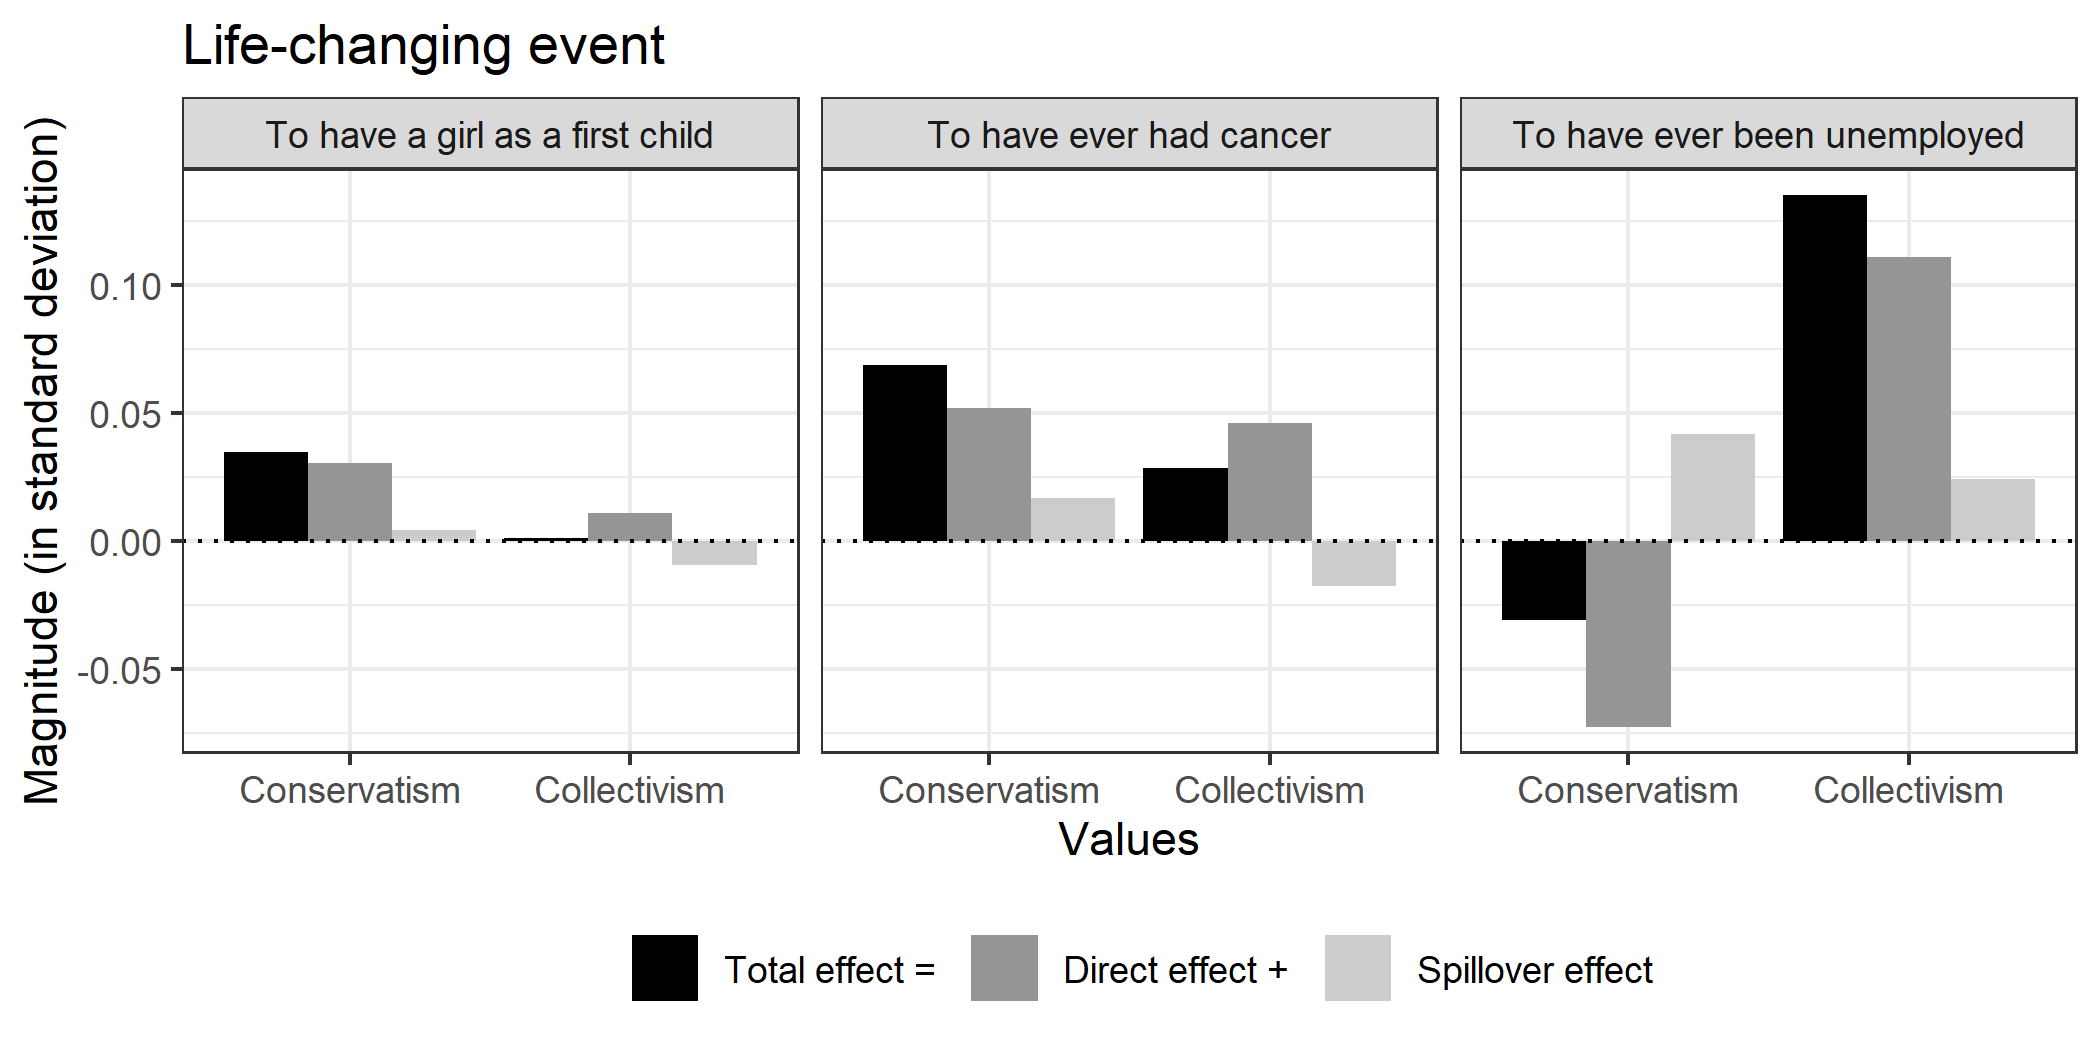
\includegraphics[width=\linewidth]{chap3/graphic/decomp-v5-base.png}
    \hrulefill
	\vspace{-3em}
	\justify\singlespacing\footnotesize{\textit{Notes:} This figure presents the decomposition of the total effect of each life-changing event on both values, Conservatism and Collectivism. The magnitude of effects is expressed in standard deviation. Decompositions are respectively derived from tables \ref{chap3-tab:decomp-GF}, \ref{chap3-tab:decomp-GC} and \ref{chap3-tab:decomp-BU}.}
\end{figure}
Having a girl as a first child directly increases conservative values by 0.03 standard deviation and collectivism by 0.01 standard deviation. Due to the consistency of values, about 14\% of the increase in conservatism is amplified by the raise in collectivism that has a positive impact on conservatism. Meanwhile, the increase in conservatism totally offsets the increase in collectivism, leading to a total effect that is negative although close to zero. Thus, due to the consistency of values and therefore the offsetting effect, collectivism does not increase when an individual gets a girl as a first child rather than a boy, while conservative values do increase. % This reconcile what we have seen in raw reg

Looking at heterogeneity across parents that are affected by this life event delivers two results (see figure \ref{chap3-fig:sem-decomp-v5-GFGender} and \ref{chap3-fig:sem-decomp-v5-GFEduc} in appendix \ref{chap3-estimates}). 
% Split by parents gender
First, for both, mothers and fathers, the direct effects go in the same direction---conservatism and collectivism---but they are more pronounced for mothers. For fathers, the negative spillover effect on collectivism offsets the positive information shock which leads to an increase in individualism. 
% Split by parents education
Second, splitting parents according to their education level shows that those with secondary education are the most affected. The effect of having a girl as a first child on tertiary-educated parents generates more progressive values which is consistent with \citet{Washington2008Female} results showing that congresspersons, hence, mostly highly educated men, become more progressive in their voting after having a daughter.

% HAVING EVER HAD CANCER
Having ever had cancer directly increases both conservatism and collectivism by 0.05 standard deviation. Due to values consistency, the increase in collectivism also increases conservative values through the spillover effect by 0.02 standard deviation, which represents almost a fourth of the total effect on conservatism. Meanwhile, part of the effect on collectivism is offset by the spillover effect of the life event through conservatism. As conservatism raises, it also decreases collectivism by 0.02 standard deviation which corresponds to 38\% of the direct effect. Thus, without the consistency of values, the increase in collectivism would have been 38\% much larger.

One may be concerned by the NCDS58 cohort at age 50 as they are likely to anticipate sickness, thus, changing their values. Excluding the NCDS58 cohort at age 50 provides very similar results with respect to the full sample, whereas considering exclusively this cohort at that age shows that the direct effect on conservatism is four times larger with respect to the baseline specification (see figure \ref{chap3-fig:sem-decomp-v5-GCNCDS58} in appendix \ref{chap3-estimates}). Interestingly, the direct effect on collectivism is much closer to zero. Thus, those who have had cancer at age 50 are not different from those who have not had one. Such an effect may be due to the anticipation of the sickness of the whole cohort at that age as they will rely more on others, hence, they increase their collectivist values. Nonetheless, the total effect on collectivism is positive---about 0.1 standard deviation---which is mostly due to the positive spillover effect on collectivism.
I also provide these estimates by focusing only on individuals who have never had cancer in the previous period (see figure \ref{chap3-fig:sem-decomp-v5-GCNever} in appendix \ref{chap3-estimates}). Although the direct effect on collectivism is larger, qualitative results hold.

% HAVING EVER BEEN UNEMPLOYED
Focusing on the third panel, those who have ever been unemployed experience a direct decline in conservatism, i.e. an increase in progressivism, by 0.07 standard deviation and a direct increase in collectivism by 0.11 standard deviation. The spillover effect of the decline in conservatism increases collectivist values by 0.02 standard deviation. Thus, collectivism raises by 22\% due to the spillover effect. Meanwhile, the increase in collectivism generates a positive spillover effect on conservative values which offsets half of the direct raise in progressivism. As a result, the increase in conservatism is dampened by the spillover effect whereas collectivism increases substantively.\footnote{In the extension of the theoretical framework in appendix \ref{chap3-model2}, I show that there is a bias when measuring the effect of an endogenous life event---such as unemployment---on values and I derive its expression. The bias does not affect the relative shares of the total effect that are due to the direct and spillover effects, nor the sign of the latter. However, the bias may affect the magnitude of the effect. In an extreme case of endogeneity of unemployment to values, the magnitudes have to be multiplied by a factor of 2/5, whereas feasible scenarii are likely to lie with a scale factor ranging from 1 (no endogeneity) to 2/3.}

One may be concerned by the current employment status that would be the driving factor for the effect of having ever been unemployed on values. I estimate the SEM using two subsamples (see figure \ref{chap3-fig:sem-decomp-v5-BUActivity} in appendix \ref{chap3-estimates}). First, I remove unemployed individuals at the time of the interview, then, I remove those out-of-work (unemployed and inactive). Both estimates do not differ with respect to the full sample one.

\subsection{Spillover effects' dynamics}

The intensity of inter-dependence between values drives the magnitude of the spillover effects of life events on values. In the SEM, the matrix $\Gamma$ captures the relation between values within the structural form. Once we consider the estimated reduced form for the decomposition, the spillover effects appear through $\Gamma^{-1}$. For instance, in the case of the girl-first life event, the $\Gamma$ matrix corresponds to
\begin{equation*}
    \Gamma = \begin{pmatrix}1 & 0.39 \\ -0.31 & 1\end{pmatrix} \implies \Gamma^{-1} = \begin{pmatrix}0.89 & -0.35 \\ 0.28 & 0.89\end{pmatrix}.
\end{equation*}
For both other life events, the coefficients in the matrices $\Gamma$ are very close to these ones which indicates that spillover effects do not depend on life events but are rather inherent.%
\footnote{See tables \ref{chap3-tab:reg-v5-sem-GC-stage12} and \ref{chap3-tab:reg-v5-sem-BU-stage12} in the appendix from which the $\Gamma$ matrix can be derived. For the got-cancer life event, $\Gamma = \begin{pmatrix}1 & 0.37 \\ -0.34 & 1\end{pmatrix}$. For the been-unmployed life event, $\Gamma = \begin{pmatrix}1 & 0.37 \\ -0.33 & 1\end{pmatrix}$.}
Thus, the effect of the life event $Z$ on values is derived from the matrix product of $\Theta = \begin{pmatrix} \theta_{Cons} & \theta_{Coll} \end{pmatrix}$ and the propagation matrix $\Gamma^{-1}$ that accounts for direct and spillover effects.

Considering the effect of the life event $Z$ on both values as a homogeneous system of first-order linear differential equations leads to
\begin{align*}
    x^\prime &= 0.89 x + 0.28 y,\\
    y^\prime &= -0.35 x + 0.89 y,
\end{align*}
where $x$ and $y$ are the magnitudes of both information shocks from $\Theta$, whereas $x^\prime$ and $y^\prime$ correspond to the net effects on values from $\Phi$. Solving this system leads to complex eigenvalues with positive real parts. This is due to the fact that, in $\Gamma$, the coefficients on the diagonal are equal to one and both off-diagonal coefficients have opposite signs. 

Figure \ref{chap3-fig:phase-plane} illustrates the phase plane of this system.
\begin{figure}[!tb]
    \centering
    \caption{Dynamics between values}
    \label{chap3-fig:phase-plane}
    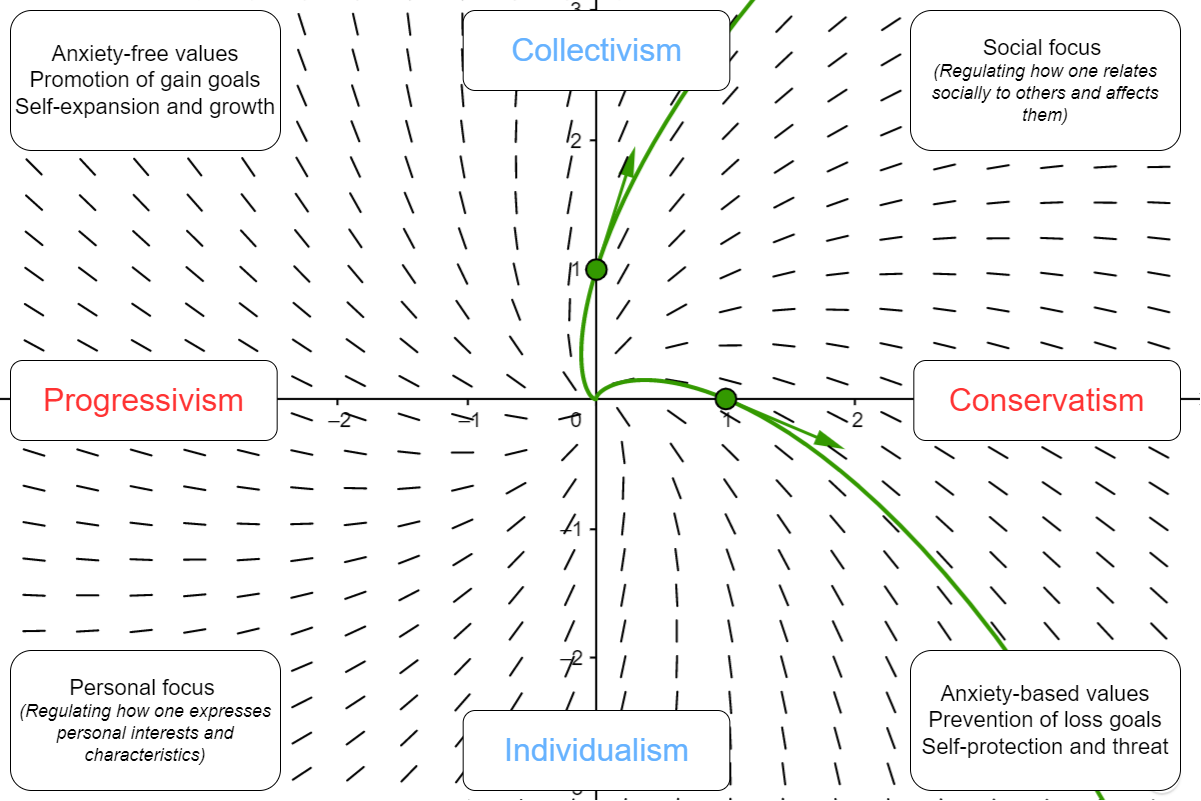
\includegraphics[width=\linewidth]{chap3/graphic/sys-diff-eq-plus.png}
	\vspace{-3em}
	\justify\singlespacing\footnotesize{\textit{Notes:} This figure presents the phase plane of the homogeneous system of first-order linear differential equations that describes the relationship between conservatism (versus progressivism) and collectivism (versus individualism) values. Green arrows decompose the direct effect and the indirect effect, i.e. spillover effect, due to a one standard deviation increase in each value.}
\end{figure}
Green dots are set to 1 on both axis, thus, the green arrows describe what happens for a one standard deviation increase on either the x-axis or the y-axis, i.e. in conservatism or in collectivism. An increase in conservatism has a negative spillover effect on collectivism, while an increase in collectivism has a positive spillover effect on conservatism. Thus, the relationship between values is \textit{not reciprocal} because of the spiral pattern in the system of first-order linear differential equations that is derived from the propagation matrix $\Gamma$.

Social psychology literature provides dynamic principles that shed light on the spiral pattern. Those principles correspond to the dynamic underpinnings of changes in values and correspond to the four corners of the figure (see \citealt{Schwartz2012Overview} for more details). For instance, any simultaneous increase in both conservatism and collectivism values, hence toward the top-right corner, refers to a raise in \textit{social focus}, i.e. preferring to live within a community and reinforcing the stability, tradition, and conformity to that community. Conversely, a decrease in those two values, hence toward the bottom-left corner, correspond to a raise in \textit{personal focus}, i.e. preferring to focus on self and not being constrained by rules. Looking at the two other corners, when individualism increases along with conservatism, hence toward the bottom-right corner, this refers to changes in values that help to deal with anxiety and the fear of loss goals, thus, they are self-protective values. Conversely, the top-left corner corresponds to self-expansive and anxiety-free based values.

Examining the spiral pattern of spillover effects through the lens of the dynamic underpinnings of value changes from social psychology provides several keys to understanding how life events affect individuals' values in figure \ref{chap3-fig:sem-decomp-v5-base}.
First, the initial increase in conservatism for both girl-first and got-cancer life events generates a spillover in individualism as those two life events are associated with anxiety, hence, self-protective values. Meanwhile, the initial raise of collectivist values reinforces the increase in conservatism by generating a positive spillover as it triggers a rise in social focus, i.e. relying more on the community and its rules.
For the been-unemployed life event, the initial increase in progressivism characterizes an increase in anxiety-free values as the fear of unemployed is not relevant anymore compared to those who have never been unemployed, hence, preventing themselves from losses. This raise in anxiety-free values has a positive impact on collectivism. The direct effect on collectivism is positive as the individual had relied more on the community since she had been unemployed, thus, this increases the social focus, hence conservative values.
    
    \section{Summary and concluding remarks} \label{chap3-conclusion}
    An extensive literature has studied the effect of life experiences on values but supposing that values are independent. I present a framework that jointly analyzes the dynamics of values over the lifecycle when life events provide information shocks on values in a context where values are inter-dependent in society. My results suggest that values inter-dependence plays an important role as individuals seek to be consistent with respect to values held in the group with which they identify. Thus, neglecting this mechanism underestimates to which extent life experiences affect individuals.

This paper has two main limitations which relate to the theoretical framework. First, I assume that value frontiers between groups are exogenous, while they are most likely endogenous. In my theoretical framework, I assume that the population is sufficiently large to ensure the anonymity of the agent, meaning that any change of value from the agent does not change the distribution. Relaxing this hypothesis would make the value frontier between groups endogenous. It would also relate the theoretical framework to the literature on network. Considering, for instance, that some individuals are more influential than others according to their position within the network. Such a framework could lead to a new approach in linking behaviors, values, and networks in a context of inter-dependence between values. Although I do not consider this approach in this paper, I intend to explore it in future works.

Second, I focus on individual life events, hence, the model is a partial equilibrium model. Thus, I suppose that values held in the group are time-invariant. An extension of the model would be to make them time-dependent, hence, sufficiently large shocks in one period, such as economic crises or global pandemics, would affect the average values. However, this extension goes beyond the scope of the paper and is also intentionally left for future research.

This paper raises an issue that has not been considered in the economic literature yet, namely, the consequences of life events on values. As values are at the roots of agents' preferences---which themselves can explain gaps in economic outcomes---, I believe that values dynamics could be incorporated in future work to explain how observed gaps between individuals can be due to differences in exposure to life events. 
    
    \printbibliography[heading=subbibintoc]
    
    \clearpage
    \addsec{Appendices}
    \renewcommand{\thesubsection}{\thechapter.\Alph{subsection}}
    
    \subsection{Model details} \label{chap3-model}
    This appendix presents the details of the theoretical framework.

\begin{proof}[Proof of Proposition \ref{chap3-prp:converge}]
    The value converges as $\lim_{t\to+\infty} a_t = a^\star$ since $(\eta_a,\phi_a)\in(\mathbb{R}^\star_{+})^2$. The rate of convergence $\eta_a/(\eta_a+\phi_a)$ is a decreasing in $\phi_a/\eta_a$. The smaller the rate of convergence, the faster the speed of convergence. Therefore, the speed of convergence is an increasing function of the relative weight of the group consistency with respect to the time consistency in the utility function.
\end{proof}

\begin{proof}[Proof of Proposition \ref{chap3-prp:shock}]
$\forall s_t\in\{\underline{s}, \overline{s}\}, \forall a_t\in\mathbb{R},~\exists \Delta{a_t} > \Delta\widetilde{a}_t$ such that $\lim_{t\to+\infty} a_{t+1} = a^\star(-s_t)$
\end{proof}

\begin{proof}[Proof of Proposition \ref{chap3-prp:relevant}]
Starting with the expression of the indifference value $\widetilde{a}$ from equation, it is straightforward to show that $\frac{\partial^2\widetilde{a}}{\partial(\overline{b}-\underline{b})^2}>0$. In this example, $\widetilde{a}$ is a convex function of $\overline{b}-\underline{b}$. Thus, the greater the gap between both groups in value $b$ with respect to value $a$, the greater the information shock in value $a$ has to be so that the agent identifies to the other group. Therefore, the less relevant is this latter value in its choice of group membership.
\end{proof}

\begin{proof}[Proof of Proposition \ref{chap3-prp:spillover}]
If $\overline{b}-\underline{b}\neq 0$, then $\exists \Delta{a_t}$ such that $a_{t-1}^\prime > \widetilde{a}_{t-1}$ which implies that the individual identifies to the other group in period $t$. Therefore, both values $a_t$ and $b_t$ change.
\end{proof}

\textbf{Theoretical framework with three groups.}
One may ask to which extent the results hold with more than two groups. So, suppose that instead of having two groups in the reference population, we introduce a third group between both groups. I refer to the former groups as $s_A$ and $s_C$ instead of $\overline{s}$ and $\underline{s}$, while $s_B$ is the new group.

Starting with the single-value model, the ranking is as follows $a_A < a_B < a_C$. Reproducing figure \ref{chap3-fig:theory-choice-a} but with three groups leads to figure \ref{chap3-fig:theory-choice3-a}.
\begin{figure}[!ht]
    \centering
    \caption{Indifference value and group membership (with three groups)}
    \label{chap3-fig:theory-choice3-a}
    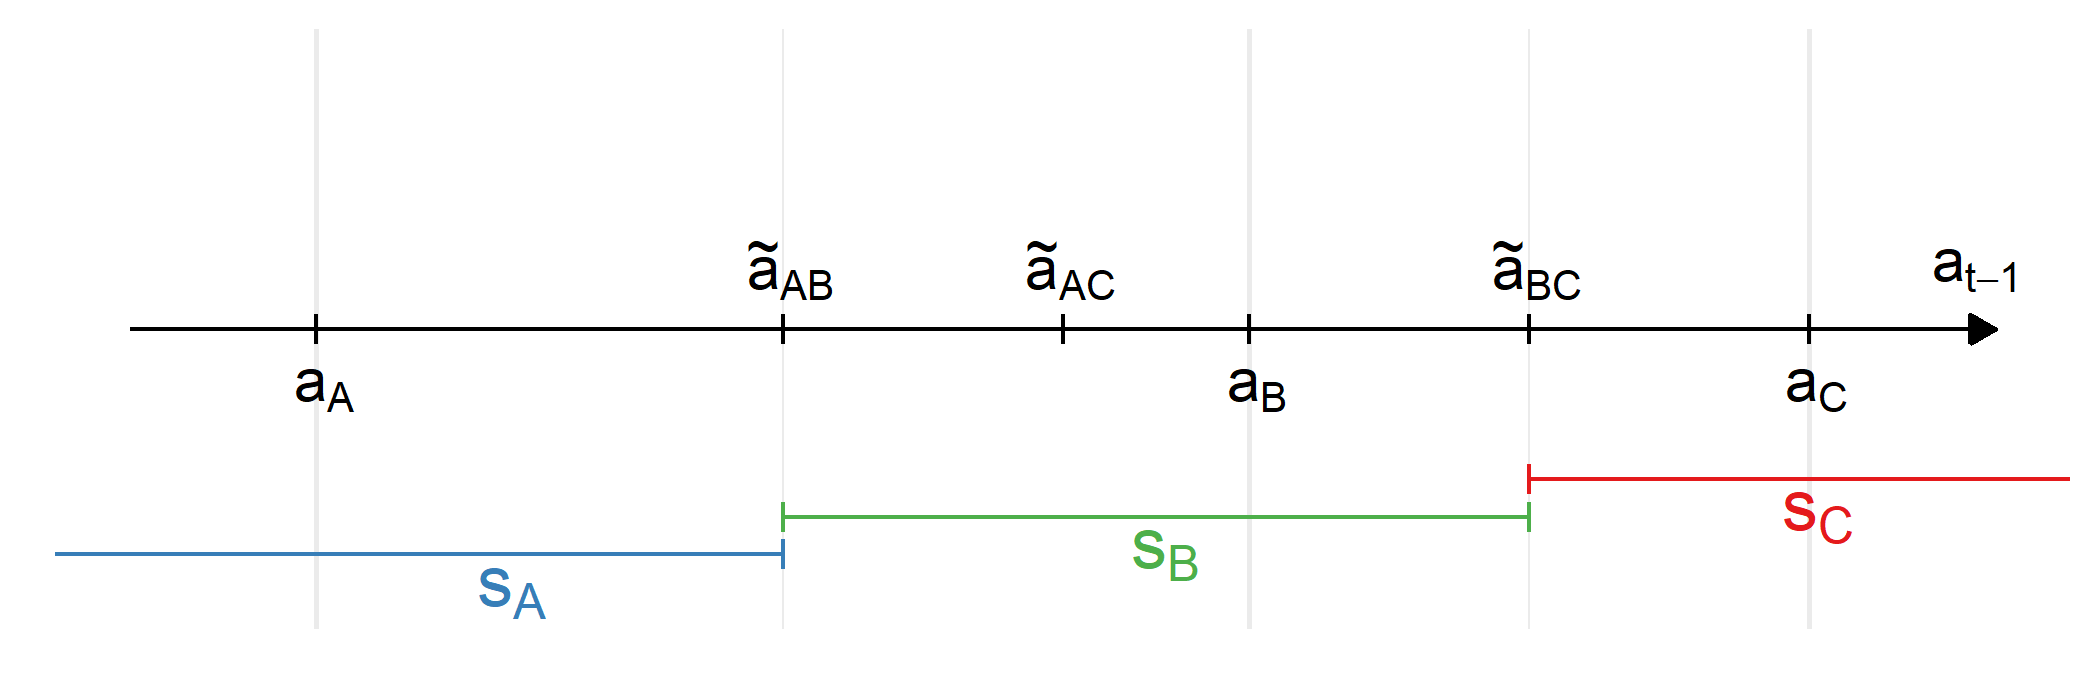
\includegraphics[width=.8\linewidth]{chap3/graphic/theory-choice3-a.png}
	\vspace{-3em}
	\justify\singlespacing\footnotesize{\textit{Notes:} This figure is an extension of figure \ref{chap3-fig:theory-choice-a} when there are three groups instead of two in the single value model. The figure presents the indifference values $\widetilde{a}_{ij}$ which are defined as the threshold values $a$ in $t-1$ such that the agent is indifferent between two groups. When the value $a$ in previous period lie in the area of one group, the agent prefers to identify to this group.}
\end{figure}
Introducing an additional group does not change the indifference value between two groups---which remains the midpoint value.
Propositions \ref{chap3-prp:converge} and \ref{chap3-prp:shock} hold in the three-group model.

Consider the two-value model by introducing the second value $b$. Assume the following ranking $a_C < a_B < a_A$ and $b_C < b_B < b_A$, which means that values are positively correlated across groups. I use the simplest case as an example, but other types of ranking are possible. Suppose the setup of section \ref{chap3-theoretical} with respect to the agent. She belongs to the group with the lowest value $a$, hence, $s_A$. It is still possible to derive the expression of the indifference value between the groups $A$ and $j\in\{B,C\}$ from equation \eqref{chap3-eq:indiff}, namely,
\begin{equation}\label{chap3-eq:indiff2}
    \widetilde{a}_{Aj} = \widehat{a}_{Aj} + \frac{1}{2\gamma}\frac{\big(b_j-b_A\big)^2}{a_j-a_A},
\end{equation}
where $\widehat{a}_{Aj}$ is the midpoint value between those of both groups $A$ and $j$. Since $a_j-a_A > 0$, it means that the second term of \eqref{chap3-eq:indiff2} is positive. As a result, the indifference value $\widetilde{a}$ is greater than the midpoint value. Both frontiers are pushed further right with respect to the single-value model in figure \ref{chap3-fig:theory-choice3-a}.

Under those conditions, it is still always possible to find an information shock such that the agent changes her group. Therefore, both propositions \ref{chap3-prp:relevant} and \ref{chap3-prp:spillover} hold. Although spillover effects still exist, their magnitudes are different with respect to the case with the two groups. Information shocks that move $a^\prime_{t-1}$ between $\widetilde{a}_{AB}$ and $\widetilde{a}_{BC}$ generate smaller spillover effects---with respect to the two-group model---as the agent identifies to the group $s_B$; while shocks that move $a^\prime_{t-1}$ beyond $\widetilde{a}_{BC}$ generate larger spillover effects.
    \clearpage
    \subsection{Statement details} \label{chap3-statement}
    This appendix presents the details of statements according to attitudes. These details have been split into three tables, namely, tables \ref{chap3-tab:statement-split-1}, \ref{chap3-tab:statement-split-2} and \ref{chap3-tab:statement-split-3}.

\begin{table}[!hb]
    \centering
    \caption{Statements details by attitudes - Part 1/3}
    \label{chap3-tab:statement-split-1}
    \resizebox*{\textwidth}{!}{
        \begin{threeparttable}
            \begin{tabular}{lll}
\toprule
Variable & Question & Rev\\
\midrule
\addlinespace[0.3em]
\multicolumn{3}{l}{\textbf{Authority (A)}}\\
\hline
\hspace{1em}A1 & The law should be obeyed, even if a particular law is wrong? & \\
\hspace{1em}A2 & For some crimes the death penalty is the most appropriate sentence? & \\
\hspace{1em}A3 & Censorship of films and magazines is necessary to uphold moral standards? & \\
\hspace{1em}A4 & People who break the law should be given stiffer sentences? & \\
\hspace{1em}A5 & Young people today don't have enough respect for traditional British values? & \\
\hspace{1em}A6 & Schools should teach children to obey authority? & \\
\addlinespace[0.3em]
\multicolumn{3}{l}{\textbf{Anti-Racism (AR)}}\\
\hline
\hspace{1em}AR1 & It is alright for people from different races to get married? & \\
\hspace{1em}AR2 & I would not mind if a family from another race moved in next door to me? & \\
\hspace{1em}AR3 & I would not mind if my child went to a school where half the children were of another race? & \\
\hspace{1em}AR4 & I would not mind working with people from other races? & \\
\hspace{1em}AR5 & I would not want a person from another race to be my boss? & X\\
\addlinespace[0.3em]
\multicolumn{3}{l}{\textbf{Children (C)}}\\
\hline
\hspace{1em}C1 & Unless you have children you'll be lonely when you get old? & \\
\hspace{1em}C2 & People can have a fulfilling life without having children? & X\\
\hspace{1em}C3 & Having children seriously interferes with the freedom of their parents? & X\\
\hspace{1em}C4 & People who never have children are missing an important part of life? & \\
\addlinespace[0.3em]
\multicolumn{3}{l}{\textbf{Environment (E)}}\\
\hline
\hspace{1em}E1 & Problems in the environment are not as serious as people claim? & X\\
\hspace{1em}E2 & We should tackle problems in the environment even if this means slower economic growth? & \\
\hspace{1em}E3 & Preserving the environment is more important than any other political issue today? & \\
\bottomrule
\end{tabular}

            \begin{tablenotes}[flushleft]
            \footnotesize{\item \textit{Notes}: The \textit{Rev} column indicates whether the scale has been reversed in the analysis.}
            \end{tablenotes}
        \end{threeparttable}
    }
\end{table}

\begin{table}[!htb]
    \centering
    \caption{Statements details by attitudes - Part 2/3}
    \label{chap3-tab:statement-split-2}
    \resizebox*{\textwidth}{!}{
        \begin{threeparttable}
            
\begin{tabular}{lll}
\toprule
Variable & Question & Rev\\
\midrule
\addlinespace[0.3em]
\multicolumn{3}{l}{\textbf{Inequality Aversion (IA)}}\\
\hline
\hspace{1em}IA1 & Big business benefits owners at the expense of the workers? & \\
\hspace{1em}IA2 & Private schools should be abolished? & \\
\hspace{1em}IA3 & Management will always try to get the better of employees if it gets the chance? & \\
\hspace{1em}IA4 & The time has come for everyone to arrange their own private health care and stop relying on the NHS? & X\\
\hspace{1em}IA5 & Ordinary working people do not get their fair share of the nation's wealth? & \\
\hspace{1em}IA6 & Government should redistribute income from the better off to those who are less well off? & \\
\hspace{1em}IA7 & There is one law for the rich and one for the poor? & \\
\addlinespace[0.3em]
\multicolumn{3}{l}{\textbf{Information Technology (IT)}}\\
\hline
\hspace{1em}IT1 & Computers at work are destroying people's skills? & X\\
\hspace{1em}IT2 & Computers enrich the lives of those who use them? & \\
\hspace{1em}IT3 & Every family should have a computer? & \\
\hspace{1em}IT4 & Learning to use a computer is more trouble than it's worth? & X\\
\addlinespace[0.3em]
\multicolumn{3}{l}{\textbf{Learning (L)}}\\
\hline
\hspace{1em}L1 & You are more likely to get a better job if you do some learning, training or education? & \\
\hspace{1em}L2 & For getting jobs, knowing the right people is more important than the qualifications? & X\\
\hspace{1em}L3 & Learning about new things boosts your confidence? & \\
\hspace{1em}L4 & The effort of getting qualifications is more trouble than it's worth? & X\\
\addlinespace[0.3em]
\multicolumn{3}{l}{\textbf{Morale (MOR)}}\\
\hline
\hspace{1em}MOR1 & Divorce is too easy to get these days? & \\
\hspace{1em}MOR2 & Married people are generally happier than unmarried people? & \\
\hspace{1em}MOR3 & Couples who have children should not separate? & \\
\hspace{1em}MOR4 & Marriage is for life? & \\
\hspace{1em}MOR5 & All women should have the right to choose an abortion if they wish? & X\\
\hspace{1em}MOR6 & It is alright for people to have children without being married? & X\\
\bottomrule
\end{tabular}

            \begin{tablenotes}[flushleft]
            \footnotesize{\item \textit{Notes}: The \textit{Rev} column indicates whether the scale has been reversed in the analysis.}
            \end{tablenotes}
        \end{threeparttable}}
\end{table}

\begin{table}[!htb]
    \centering
    \caption{Statements details by attitudes - Part 3/3}
    \label{chap3-tab:statement-split-3}
    \resizebox*{\textwidth}{!}{
        \begin{threeparttable}
            
\begin{tabular}{lll}
\toprule
Variable & Question & Rev\\
\midrule
\addlinespace[0.3em]
\multicolumn{3}{l}{\textbf{Political Cynicism (PC)}}\\
\hline
\hspace{1em}PC1 & None of the political parties would do anything to benefit me? & \\
\hspace{1em}PC2 & It does not really make much difference which political party is in power in Britain? & \\
\hspace{1em}PC3 & Politicians are mainly in politics for their own benefit and not for the benefit of the community? & \\
\addlinespace[0.3em]
\multicolumn{3}{l}{\textbf{Work-Ethic (WE)}}\\
\hline
\hspace{1em}WE1 & Having almost any job is better than being unemployed? & \\
\hspace{1em}WE2 & If I didn't like a job I'd pack it in, even if there was no other job to go to? & X\\
\hspace{1em}WE3 & Once you've got a job it's important to hang on to it even if you don't really like it? & \\
\addlinespace[0.3em]
\multicolumn{3}{l}{\textbf{Working Mother (WM)}}\\
\hline
\hspace{1em}WM1 & A pre-school child is likely to suffer if his or her mother works? & X\\
\hspace{1em}WM2 & All in all, family life suffers when the mother has a full time job? & X\\
\hspace{1em}WM3 & Children benefit if their mother has a job outside the home? & \\
\hspace{1em}WM4 & A mother and her family will all be happier if she goes out to work? & \\
\hspace{1em}WM5 & A father's job is to earn money; a mother's job is to look after the home and family? & X\\
\bottomrule
\end{tabular}

            \begin{tablenotes}[flushleft]
            \footnotesize{\item \textit{Notes}: The \textit{Rev} column indicates whether the scale has been reversed in the analysis.}
            \end{tablenotes}
        \end{threeparttable}}
\end{table}

    \clearpage
    \subsection{Principal component analysis} \label{chap3-pca}
    This appendix presents the principal components eigenvectors from the Principal Component Analysis (PCA) in section \ref{chap3-data}. Table \ref{chap3-tab:pca-v5-BCS70} presents the eigenvectors for the BCS70 cohort, while table \ref{chap3-tab:pca-v5-NCDS58} displays those for the NCDS58 cohort.

\begin{table}[!hb]
    \centering
    \caption{Principal components eigenvectors for the BCS70 cohort}
    \label{chap3-tab:pca-v5-BCS70}
    \begin{threeparttable}
        
\begin{tabular}{lrrrrr}
\toprule
  & \multicolumn{1}{c}{PC1} & \multicolumn{1}{c}{PC2} & \multicolumn{1}{c}{PC3} & \multicolumn{1}{c}{PC4} & \multicolumn{1}{c}{PC5}\\
\midrule
\addlinespace[0.3em]
\multicolumn{6}{l}{\textbf{Age 26}}\\
\hline
\hspace{1em}Authority & 0.622 & 0.011 & 0.136 & -0.146 & -0.757\\
\hspace{1em}Inequality Aversion & -0.182 & 0.686 & -0.533 & 0.348 & -0.303\\
\hspace{1em}Morale & 0.521 & 0.244 & -0.453 & -0.513 & 0.449\\
\hspace{1em}Political Cynicism & 0.149 & 0.656 & 0.695 & 0.065 & 0.245\\
\hspace{1em}Work Ethic & 0.535 & -0.200 & -0.093 & 0.769 & 0.272\\
\midrule
\hspace{1em}Standard deviation & 1.262 & 1.087 & 0.929 & 0.866 & 0.783\\
\hspace{1em}Proportion of Variance & 0.319 & 0.236 & 0.173 & 0.150 & 0.123\\
\hspace{1em}Cumulative Proportion & 0.319 & 0.555 & 0.727 & 0.877 & 1.000\\
\addlinespace[0.3em]
\multicolumn{6}{l}{\textbf{Age 30}}\\
\hline
\hspace{1em}Authority & 0.614 & -0.162 & -0.050 & 0.281 & -0.718\\
\hspace{1em}Inequality Aversion & 0.153 & 0.702 & 0.013 & -0.638 & -0.278\\
\hspace{1em}Morale & 0.534 & -0.109 & -0.678 & -0.202 & 0.450\\
\hspace{1em}Political Cynicism & 0.326 & 0.605 & 0.221 & 0.592 & 0.359\\
\hspace{1em}Work Ethic & 0.456 & -0.321 & 0.699 & -0.351 & 0.276\\
\midrule
\hspace{1em}Standard deviation & 1.243 & 1.137 & 0.918 & 0.827 & 0.797\\
\hspace{1em}Proportion of Variance & 0.309 & 0.259 & 0.169 & 0.137 & 0.127\\
\hspace{1em}Cumulative Proportion & 0.309 & 0.568 & 0.736 & 0.873 & 1.000\\
\addlinespace[0.3em]
\multicolumn{6}{l}{\textbf{Age 42}}\\
\hline
\hspace{1em}Authority & 0.570 & -0.360 & -0.004 & -0.519 & -0.526\\
\hspace{1em}Inequality Aversion & 0.172 & 0.722 & 0.172 & 0.280 & -0.584\\
\hspace{1em}Morale & 0.462 & -0.048 & -0.749 & 0.466 & 0.079\\
\hspace{1em}Political Cynicism & 0.517 & 0.474 & 0.122 & -0.368 & 0.598\\
\hspace{1em}Work Ethic & 0.406 & -0.350 & 0.628 & 0.548 & 0.135\\
\midrule
\hspace{1em}Standard deviation & 1.184 & 1.124 & 0.968 & 0.882 & 0.787\\
\hspace{1em}Proportion of Variance & 0.281 & 0.253 & 0.187 & 0.156 & 0.124\\
\hspace{1em}Cumulative Proportion & 0.281 & 0.533 & 0.721 & 0.876 & 1.000\\
\bottomrule
\end{tabular}

        % \begin{tablenotes}[flushleft]
        %     \footnotesize{\item \textit{Notes}: Signs of the eigenvectors have been inverted for age 30 and age 42 in order to have the same axis direction for the first principal component. The attitude toward Inequality Aversion (IA) is removed for the PCA on the BCS70 cohort at the age of 26 years because only one statement is available.}
        % \end{tablenotes}
    \end{threeparttable}
\end{table}

\begin{table}[!htb]
    \centering
    \caption{Principal components eigenvectors for the NCDS58 cohort}
    \label{chap3-tab:pca-v5-NCDS58}
    \begin{threeparttable}
        
\begin{tabular}{lrrrrr}
\toprule
  & \multicolumn{1}{c}{PC1} & \multicolumn{1}{c}{PC2} & \multicolumn{1}{c}{PC3} & \multicolumn{1}{c}{PC4} & \multicolumn{1}{c}{PC5}\\
\midrule
\addlinespace[0.3em]
\multicolumn{6}{l}{\textbf{Age 33}}\\
\hline
\hspace{1em}Authority & 0.607 & -0.150 & 0.155 & -0.546 & 0.535\\
\hspace{1em}Inequality Aversion & 0.006 & 0.730 & -0.072 & 0.353 & 0.580\\
\hspace{1em}Morale & 0.548 & -0.077 & 0.551 & 0.591 & -0.201\\
\hspace{1em}Political Cynicism & 0.276 & 0.654 & 0.053 & -0.414 & -0.567\\
\hspace{1em}Work Ethic & 0.504 & -0.102 & -0.815 & 0.237 & -0.122\\
\midrule
\hspace{1em}Standard deviation & 1.250 & 1.162 & 0.901 & 0.851 & 0.741\\
\hspace{1em}Proportion of Variance & 0.313 & 0.270 & 0.162 & 0.145 & 0.110\\
\hspace{1em}Cumulative Proportion & 0.313 & 0.583 & 0.745 & 0.890 & 1.000\\
\addlinespace[0.3em]
\multicolumn{6}{l}{\textbf{Age 42}}\\
\hline
\hspace{1em}Authority & 0.605 & -0.141 & -0.156 & 0.369 & 0.674\\
\hspace{1em}Inequality Aversion & 0.173 & 0.713 & 0.178 & -0.559 & 0.342\\
\hspace{1em}Morale & 0.500 & -0.245 & -0.542 & -0.534 & -0.333\\
\hspace{1em}Political Cynicism & 0.446 & 0.521 & 0.038 & 0.480 & -0.546\\
\hspace{1em}Work Ethic & 0.395 & -0.375 & 0.805 & -0.187 & -0.144\\
\midrule
\hspace{1em}Standard deviation & 1.258 & 1.101 & 0.916 & 0.875 & 0.775\\
\hspace{1em}Proportion of Variance & 0.317 & 0.242 & 0.168 & 0.153 & 0.120\\
\hspace{1em}Cumulative Proportion & 0.317 & 0.559 & 0.727 & 0.880 & 1.000\\
\addlinespace[0.3em]
\multicolumn{6}{l}{\textbf{Age 50}}\\
\hline
\hspace{1em}Authority & 0.531 & -0.134 & 0.063 & -0.816 & -0.173\\
\hspace{1em}Inequality Aversion & 0.554 & 0.296 & -0.075 & 0.441 & -0.637\\
\hspace{1em}Morale & 0.157 & -0.663 & -0.716 & 0.152 & 0.018\\
\hspace{1em}Political Cynicism & 0.578 & 0.264 & -0.063 & 0.170 & 0.750\\
\hspace{1em}Work Ethic & 0.229 & -0.620 & 0.689 & 0.296 & 0.033\\
\midrule
\hspace{1em}Standard deviation & 1.373 & 1.046 & 0.945 & 0.804 & 0.694\\
\hspace{1em}Proportion of Variance & 0.377 & 0.219 & 0.179 & 0.129 & 0.096\\
\hspace{1em}Cumulative Proportion & 0.377 & 0.596 & 0.775 & 0.904 & 1.000\\
\bottomrule
\end{tabular}

        % \begin{tablenotes}[flushleft]
        %     \footnotesize{\item \textit{Notes}: Signs of eigenvectors have been inverted for age 33 and age 50 in order to have the same axis direction for the first principal component.}
        % \end{tablenotes}
    \end{threeparttable}
\end{table}

\begin{figure}[!htb]
    \caption{Two-dimensional structure of universal motivational types of values}
    \label{chap3-fig:schwartz}
    \centering
    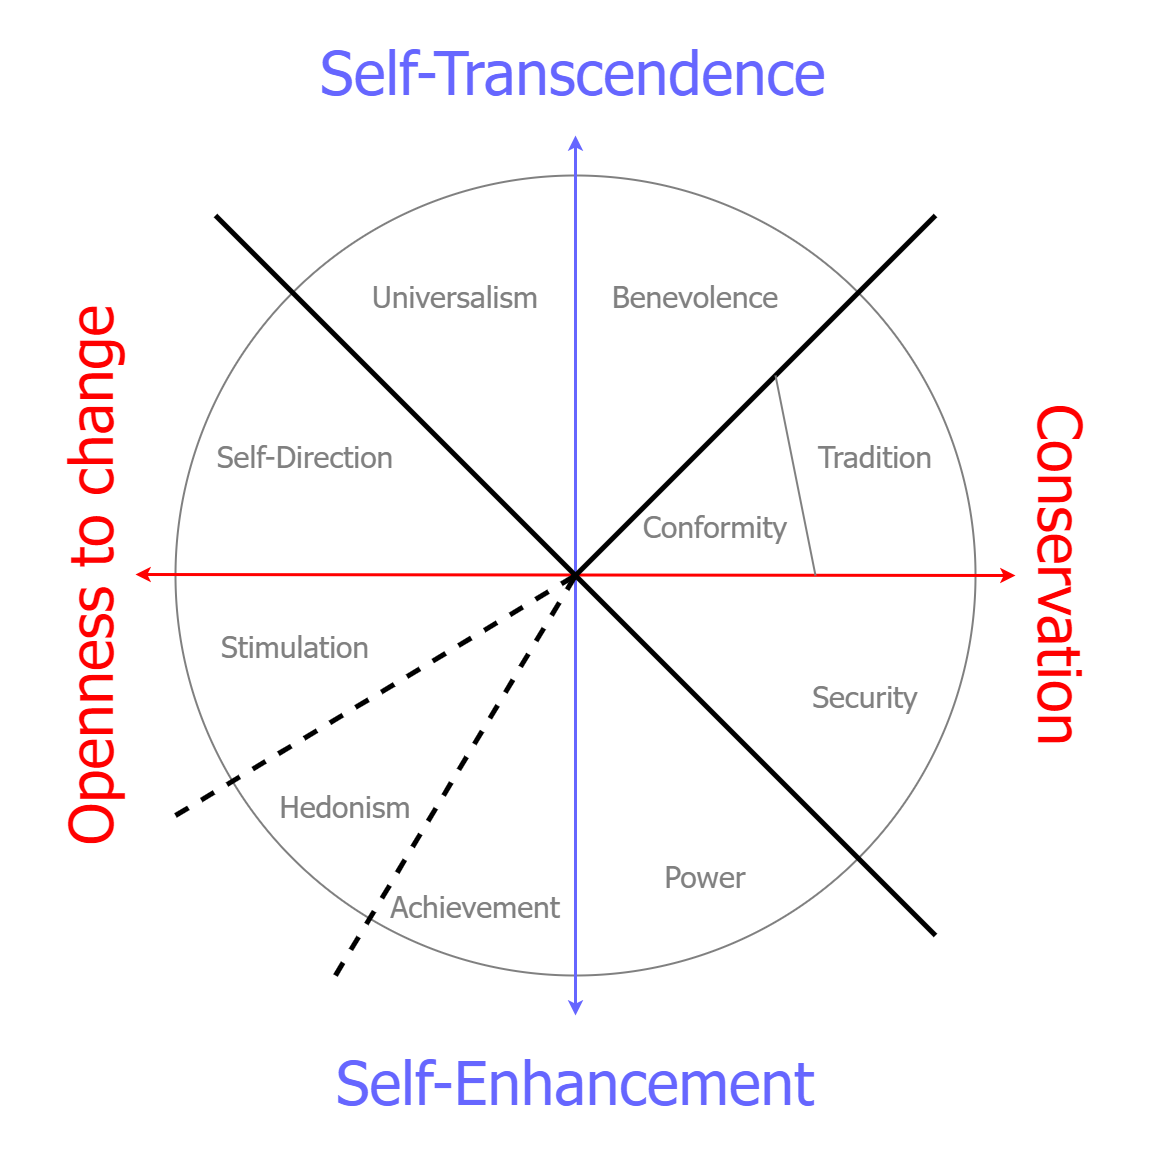
\includegraphics[width=.8\linewidth]{chap3/graphic/schwartz92.png}
	\vspace{-3em}
	\justify\singlespacing\footnotesize{\textit{Notes:} This figure reproduces the two-dimensional structure of motivational types of values from \citet{Schwartz1992Universals, Schwartz2012Overview}.}
\end{figure}
    \clearpage
    \subsection{Data details} \label{chap3-details}
    This appendix presents the details of the data. Table \ref{chap3-tab:data-vote} shows the shares of vote in general elections in both cohorts.

\begin{table}[!htb]
    \centering
    \caption{Shares of vote in general elections in both cohorts}
    \label{chap3-tab:data-vote}
    \begin{threeparttable}
        % \setlength{\tabcolsep}{5pt}
        
\begin{tabular}{llrrrrrr}
\toprule
\multicolumn{1}{c}{} & \multicolumn{1}{c}{} & \multicolumn{6}{c}{Proportion of total (in percent)} \\
\cmidrule(l{3pt}r{3pt}){3-8}
  &   & Other & Con & Grn & Lab & LD & UKIP\\
\midrule
BCS70 & Age 26 (GE 1997) & 45.5 & 15.6 & 0.5 & 30.8 & 7.6 & \\
BCS70 & Age 30 (GE 2001) & 51.6 & 13.0 & 1.0 & 25.8 & 7.8 & 0.8\\
BCS70 & Age 42 (GE 2010) & 30.4 & 28.8 & 1.7 & 23.1 & 14.3 & 1.7\\
\midrule
NCDS58 & Age 33 (GE 1987) & 27.6 & 34.0 &  & 26.8 & 11.6 & \\
NCDS58 & Age 42 (GE 1997) & 27.6 & 21.5 & 0.6 & 40.5 & 9.8 & \\
NCDS58 & Age 50 (GE 2010) & 43.2 & 22.9 & 1.1 & 19.0 & 10.8 & 3.0\\
\bottomrule
\end{tabular}

        \begin{tablenotes}[flushleft]
            \footnotesize{\item \textit{Notes}: This table presents the vote proportions (in percentage) for both cohorts at different ages according to the closest General Election (GE). Political parties are (in alphabetical order): Conservative (Con), Green (Grn), Labour (Lab), Liberal Democrat (LD), and UK Independence Party (UKIP). Other encompasses all other parties, blank votes and abstention.}
        \end{tablenotes}
    \end{threeparttable}
\end{table}
    \clearpage
    \subsection{Estimates} \label{chap3-estimates}
    This appendix presents additional regression tables of the paper. 
% RAW ESTIMATE
Table \ref{chap3-tab:reg-v5-raw-all-long} presents the long-version table of the regression table \ref{chap3-tab:reg-v5-raw-all-short} in the paper.
% INSTRUMENTAL VARIABLE
Table \ref{chap3-tab:reg-v5-IV-GFGC-long} presents the IV estimate of the spillover effects. Tables \ref{chap3-tab:reg-v5-IV-GFvote} and \ref{chap3-tab:reg-v5-IV-GCvote} correspond to the IV estimate of the group membership.
% SEM
Table \ref{chap3-tab:reg-v5-sem-GF-stage12}, \ref{chap3-tab:reg-v5-sem-GC-stage12}, and \ref{chap3-tab:reg-v5-sem-BU-stage12} present the details of the 2SLS estimates of the SEM for, respectively, the girl-first, got-cancer, and been-unemployed life event.
% DECOMPOSITION
Tables \ref{chap3-tab:decomp-GF}, \ref{chap3-tab:decomp-GC}, and \ref{chap3-tab:decomp-BU} summarize the decomposition of the total effect from the SEM for, respectively, the girl-first, got-cancer, and been-unemployed life event.
% ROBUSTNESS
Figure \ref{chap3-fig:sem-decomp-v5-GFGender} summarizes the decomposition of the total
effect of girl-first life event by parent. 
Figure \ref{chap3-fig:sem-decomp-v5-GFEduc} summarizes the decomposition of the total
effect of girl-first life event by education level.
Figure \ref{chap3-fig:sem-decomp-v5-BUActivity} summarizes the decomposition of the total
effect of been-unemployed life event according to the current activity status.

%%%%% APPLIED %%%%%

\begin{table}[!htb]
    \centering
    \caption{Effect of life events on values}
    \label{chap3-tab:reg-v5-raw-all-long}
    % \resizebox*{\textwidth}{!}{
    \begin{threeparttable}
        \setlength{\tabcolsep}{0pt}
        \begin{tabular}{l D{.}{.}{5.5} D{.}{.}{5.5} D{.}{.}{5.5} D{.}{.}{5.5} D{.}{.}{5.5} D{.}{.}{5.5}}
\toprule
 & \multicolumn{6}{c}{Linear regression - OLS} \\
\cmidrule(lr){2-7}
 & \multicolumn{2}{c}{GirlFirst} & \multicolumn{2}{c}{GotCancer} & \multicolumn{2}{c}{BeenUnemp} \\
\cmidrule(lr){2-3}\cmidrule(lr){4-5}\cmidrule(lr){6-7}
 & \multicolumn{1}{c}{(Cons)} & \multicolumn{1}{c}{(Coll)} & \multicolumn{1}{c}{(Cons)} & \multicolumn{1}{c}{(Coll)} & \multicolumn{1}{c}{(Cons)} & \multicolumn{1}{c}{(Coll)} \\
\midrule
Intercept       & 0.32^{***}  & -0.15^{***} & 0.27^{***}  & -0.07^{***} & 0.26^{***}  & -0.11^{***} \\
                & (0.02)      & (0.02)      & (0.01)      & (0.01)      & (0.01)      & (0.01)      \\
Female          & -0.19^{***} & 0.07^{***}  & -0.17^{***} & 0.02        & -0.17^{***} & 0.03^{***}  \\
                & (0.01)      & (0.01)      & (0.01)      & (0.01)      & (0.01)      & (0.01)      \\
Educ. Secondary & -0.29^{***} & -0.04^{**}  & -0.28^{***} & -0.03^{**}  & -0.28^{***} & -0.03^{**}  \\
                & (0.02)      & (0.02)      & (0.01)      & (0.01)      & (0.01)      & (0.01)      \\
Educ. Tertiary  & -0.52^{***} & -0.04^{**}  & -0.50^{***} & -0.03^{**}  & -0.50^{***} & -0.03^{***} \\
                & (0.02)      & (0.02)      & (0.01)      & (0.01)      & (0.01)      & (0.01)      \\
Life event      & 0.03^{**}   & 0.00        & 0.09^{***}  & 0.02        & 0.02^{*}    & 0.18^{***}  \\
                & (0.01)      & (0.01)      & (0.03)      & (0.03)      & (0.01)      & (0.01)      \\
Value$_{t-1}$   & 0.54^{***}  & 0.49^{***}  & 0.56^{***}  & 0.50^{***}  & 0.56^{***}  & 0.49^{***}  \\
                & (0.01)      & (0.01)      & (0.00)      & (0.00)      & (0.00)      & (0.00)      \\
\midrule
R$^2$ & \multicolumn{1}{c}{0.37} & \multicolumn{1}{c}{0.26} & \multicolumn{1}{c}{0.39} & \multicolumn{1}{c}{0.27} & \multicolumn{1}{c}{0.39} & \multicolumn{1}{c}{0.27}\\
Adj. R$^2$ & \multicolumn{1}{c}{0.37} & \multicolumn{1}{c}{0.26} & \multicolumn{1}{c}{0.39} & \multicolumn{1}{c}{0.27} & \multicolumn{1}{c}{0.39} & \multicolumn{1}{c}{0.27}\\
Num. obs. & \multicolumn{1}{c}{23354} & \multicolumn{1}{c}{23354} & \multicolumn{1}{c}{32885} & \multicolumn{1}{c}{32885} & \multicolumn{1}{c}{32885} & \multicolumn{1}{c}{32885}\\
\bottomrule
\end{tabular}

        \begin{tablenotes}[flushleft]
            \footnotesize{\item \textit{Notes}: $^{***}p<0.01$; $^{**}p<0.05$; $^{*}p<0.1$. Standard errors between parentheses. Male in the NCDS cohort in his forties with primary education as the reference group. GirlFirst and GotCancer are the life events. In GirlFirst regressions, parents who have had a boy as a first child are the reference group. In GotCancer regressions, individuals who never had a cancer are the reference group. In BeenUnemp, individuals who have never been unemployed are the reference group. Table \ref{chap3-tab:reg-v5-raw-all-short} in the paper summarizes the coefficients.}
        \end{tablenotes}
    \end{threeparttable}
    % }
\end{table}

\begin{table}[!htb]
    \centering
    \caption{IV Estimate of the spillover effect}
    \label{chap3-tab:reg-v5-IV-GFGC-long}
    \begin{threeparttable}
        \begin{tabular}{l D{.}{.}{5.5} D{.}{.}{5.5} D{.}{.}{5.5} D{.}{.}{5.5}}
\toprule
 & \multicolumn{4}{c}{IV regression - 2SLS} \\
\cmidrule(lr){2-5}
 & \multicolumn{2}{c}{GirlFirst} & \multicolumn{2}{c}{GotCancer} \\
\cmidrule(lr){2-3}\cmidrule(lr){4-5}
 & \multicolumn{1}{c}{(Cons)} & \multicolumn{1}{c}{(Coll)} & \multicolumn{1}{c}{(Cons)} & \multicolumn{1}{c}{(Coll)} \\
\midrule
Intercept                 & 0.32^{***}  & 0.07^{***}  & 0.27^{***}  & 0.10^{***}  \\
                          & (0.02)      & (0.02)      & (0.01)      & (0.01)      \\
Female                    & -0.19^{***} & -0.02^{**}  & -0.17^{***} & -0.06^{***} \\
                          & (0.01)      & (0.01)      & (0.01)      & (0.01)      \\
Educ. Secondary           & -0.29^{***} & -0.18^{***} & -0.28^{***} & -0.19^{***} \\
                          & (0.02)      & (0.02)      & (0.01)      & (0.01)      \\
Educ. Tertiary            & -0.52^{***} & -0.33^{***} & -0.50^{***} & -0.36^{***} \\
                          & (0.02)      & (0.02)      & (0.01)      & (0.01)      \\
Life event                & 0.03^{**}   &             & 0.09^{***}  &             \\
                          & (0.01)      &             & (0.03)      &             \\
$\widehat{\text{Cons}}_t$ &             & -0.32^{***} &             & -0.34^{***} \\
                          &             & (0.01)      &             & (0.01)      \\
Value$_{t-1}$             & 0.54^{***}  & 0.48^{***}  & 0.56^{***}  & 0.49^{***}  \\
                          & (0.01)      & (0.01)      & (0.00)      & (0.00)      \\
\midrule
R$^2$ & \multicolumn{1}{c}{0.37} & \multicolumn{1}{c}{0.30} & \multicolumn{1}{c}{0.39} & \multicolumn{1}{c}{0.31}\\
Adj. R$^2$ & \multicolumn{1}{c}{0.37} & \multicolumn{1}{c}{0.30} & \multicolumn{1}{c}{0.39} & \multicolumn{1}{c}{0.31}\\
Num. obs. & \multicolumn{1}{c}{23354} & \multicolumn{1}{c}{23354} & \multicolumn{1}{c}{32885} & \multicolumn{1}{c}{32885}\\
\bottomrule
\end{tabular}

        \begin{tablenotes}[flushleft]
            \footnotesize{\item \textit{Notes}: $^{***}p<0.01$; $^{**}p<0.05$; $^{*}p<0.1$. Standard errors between parentheses. Control variables include gender, education (primary, secondary, tertiary), cohort fixed effects and period fixed effects. Male in the NCDS cohort in his forties with primary education as the reference group. GirlFirst and GotCancer are the life events. In GirlFirst regressions, parents who have had a boy as a first child are the reference group. In GotCancer regressions, individuals who never had a cancer are the reference group. Table \ref{chap3-tab:reg-v5-IV-GFGC-short} in the paper summarizes the coefficients.}
        \end{tablenotes}
    \end{threeparttable}
    % }
\end{table}

\begin{table}[!htb]
    \centering
    \caption{IV Estimate of the group membership (GirlFirst)}
    \label{chap3-tab:reg-v5-IV-GFvote}
    \begin{threeparttable}
        \setlength{\tabcolsep}{3pt}
        \begin{tabular}{l D{.}{.}{5.5} D{.}{.}{5.5} D{.}{.}{5.5} D{.}{.}{5.5} D{.}{.}{5.5}}
\toprule
 & \multicolumn{5}{c}{IV regression - GirlFirst - Multinomial logit - Dep. var.: Vote} \\
\cmidrule(lr){2-6}
 & \multicolumn{1}{c}{(Con)} & \multicolumn{1}{c}{(Grn)} & \multicolumn{1}{c}{(Lab)} & \multicolumn{1}{c}{(LD)} & \multicolumn{1}{c}{(UKIP)} \\
\midrule
Intercept                 & -1.41^{***} & -3.58^{***} & -1.10^{***} & -1.98^{***} & -5.08      \\
                          & (0.04)      & (0.14)      & (0.04)      & (0.05)      & (3.22)     \\
Female                    & -0.15^{***} & 0.04        & -0.04       & -0.02       & -0.27^{**} \\
                          & (0.04)      & (0.15)      & (0.04)      & (0.05)      & (0.12)     \\
Educ. Secondary           & 0.56^{***}  & 0.35^{*}    & 0.09^{*}    & 0.55^{***}  & 0.08       \\
                          & (0.05)      & (0.20)      & (0.05)      & (0.07)      & (0.16)     \\
Educ. Tertiary            & 0.78^{***}  & 0.62^{***}  & 0.36^{***}  & 0.94^{***}  & -0.22      \\
                          & (0.06)      & (0.19)      & (0.06)      & (0.07)      & (0.20)     \\
$\widehat{\text{Cons}}_t$ & 0.01        & -0.85^{***} & -0.27^{***} & -0.34^{***} & 0.18^{*}   \\
                          & (0.03)      & (0.10)      & (0.03)      & (0.04)      & (0.09)     \\
Con $\text{Vote}_{t-1}$   & 2.56^{***}  & 0.13        & 0.46^{***}  & 0.91^{***}  & 1.27^{***} \\
                          & (0.05)      & (0.27)      & (0.06)      & (0.08)      & (0.18)     \\
Grn $\text{Vote}_{t-1}$   & 0.63^{*}    & 3.75^{***}  & 0.77^{**}   & 1.59^{***}  & 0.49       \\
                          & (0.33)      & (0.31)      & (0.35)      & (0.31)      & (1.03)     \\
Lab $\text{Vote}_{t-1}$   & 0.50^{***}  & 0.81^{***}  & 2.19^{***}  & 1.01^{***}  & 1.14^{***} \\
                          & (0.06)      & (0.18)      & (0.05)      & (0.07)      & (0.15)     \\
LD $\text{Vote}_{t-1}$    & 1.06^{***}  & 1.02^{***}  & 1.08^{***}  & 2.73^{***}  & 1.71^{***} \\
                          & (0.08)      & (0.25)      & (0.08)      & (0.08)      & (0.20)     \\
UKIP $\text{Vote}_{t-1}$  & 1.57^{***}  & 1.46        & -0.02       & 1.21^{**}   & 3.25^{***} \\
                          & (0.38)      & (1.06)      & (0.66)      & (0.50)      & (0.49)     \\
\midrule
Num. obs. & \multicolumn{1}{c}{23354} & \multicolumn{1}{c}{23354} & \multicolumn{1}{c}{23354} & \multicolumn{1}{c}{23354} & \multicolumn{1}{c}{23354}\\
\bottomrule
\end{tabular}

        \begin{tablenotes}[flushleft]
            \footnotesize{\item \textit{Notes}: $^{***}p<0.01$; $^{**}p<0.05$; $^{*}p<0.1$. Standard errors between parentheses. Control variables include gender, education (primary, secondary, tertiary), cohort fixed effects and period fixed effects. Male in the NCDS cohort in his forties with primary education as the reference group. GirlFirst and GotCancer are the life events. Parents who have had a boy as a first child are the reference group.
            % Multinomial
            The baseline outcome of the multinomial logistic regression is the vote for Other (encompassing all other parties, blank votes and abstention). $\text{Vote}_{t-1}$ corresponds to the effect of having voted for the corresponding party in the previous period.
            Table \ref{chap3-tab:reg-v5-IV-GFGCvote-short} in the paper summarizes the coefficients.}
        \end{tablenotes}
    \end{threeparttable}
    % }
\end{table}

\begin{table}[!htb]
    \centering
    \caption{IV Estimate of the group membership (GotCancer)}
    \label{chap3-tab:reg-v5-IV-GCvote}
    \begin{threeparttable}
        \setlength{\tabcolsep}{3pt}
        \begin{tabular}{l D{.}{.}{5.5} D{.}{.}{5.5} D{.}{.}{5.5} D{.}{.}{5.5} D{.}{.}{5.5}}
\toprule
 & \multicolumn{5}{c}{IV regression - GotCancer - Multinomial logit - Dep. var.: Vote} \\
\cmidrule(lr){2-6}
 & \multicolumn{1}{c}{(Con)} & \multicolumn{1}{c}{(Grn)} & \multicolumn{1}{c}{(Lab)} & \multicolumn{1}{c}{(LD)} & \multicolumn{1}{c}{(UKIP)} \\
\midrule
Intercept                 & -1.43^{***} & -3.47^{***} & -1.19^{***} & -1.97^{***} & -5.49       \\
                          & (0.03)      & (0.10)      & (0.03)      & (0.04)      & (11.53)     \\
Female                    & -0.09^{***} & 0.08        & 0.03        & 0.06        & -0.28^{***} \\
                          & (0.03)      & (0.11)      & (0.03)      & (0.04)      & (0.10)      \\
Educ. Secondary           & 0.58^{***}  & 0.23        & 0.09^{**}   & 0.50^{***}  & 0.06        \\
                          & (0.04)      & (0.16)      & (0.04)      & (0.06)      & (0.13)      \\
Educ. Tertiary            & 0.74^{***}  & 0.65^{***}  & 0.36^{***}  & 0.88^{***}  & -0.22       \\
                          & (0.05)      & (0.14)      & (0.04)      & (0.06)      & (0.16)      \\
$\widehat{\text{Cons}}_t$ & 0.08^{***}  & -0.67^{***} & -0.24^{***} & -0.32^{***} & 0.19^{**}   \\
                          & (0.03)      & (0.07)      & (0.02)      & (0.03)      & (0.07)      \\
Con $\text{Vote}_{t-1}$   & 2.56^{***}  & 0.09        & 0.47^{***}  & 0.82^{***}  & 1.22^{***}  \\
                          & (0.04)      & (0.21)      & (0.05)      & (0.07)      & (0.15)      \\
Grn $\text{Vote}_{t-1}$   & 0.29        & 3.31^{***}  & 0.36        & 1.24^{***}  & 1.28^{***}  \\
                          & (0.25)      & (0.23)      & (0.27)      & (0.23)      & (0.48)      \\
Lab $\text{Vote}_{t-1}$   & 0.41^{***}  & 0.73^{***}  & 2.21^{***}  & 0.99^{***}  & 0.87^{***}  \\
                          & (0.05)      & (0.14)      & (0.04)      & (0.06)      & (0.13)      \\
LD $\text{Vote}_{t-1}$    & 1.00^{***}  & 1.17^{***}  & 1.11^{***}  & 2.71^{***}  & 1.54^{***}  \\
                          & (0.07)      & (0.18)      & (0.06)      & (0.06)      & (0.16)      \\
UKIP $\text{Vote}_{t-1}$  & 1.46^{***}  & 1.60^{**}   & -0.03       & 1.28^{***}  & 3.06^{***}  \\
                          & (0.32)      & (0.77)      & (0.57)      & (0.41)      & (0.42)      \\
\midrule
Num. obs. & \multicolumn{1}{c}{32885} & \multicolumn{1}{c}{32885} & \multicolumn{1}{c}{32885} & \multicolumn{1}{c}{32885} & \multicolumn{1}{c}{32885}\\
\bottomrule
\end{tabular}

        \begin{tablenotes}[flushleft]
            \footnotesize{\item \textit{Notes}: $^{***}p<0.01$; $^{**}p<0.05$; $^{*}p<0.1$. Standard errors between parentheses. Control variables include gender, education (primary, secondary, tertiary), cohort fixed effects and period fixed effects. Male in the NCDS cohort in his forties with primary education as the reference group. GirlFirst and GotCancer are the life events. Individuals who never had a cancer are the reference group.
            % Multinomial
            The baseline outcome of the multinomial logistic regression is the vote for Other (encompassing all other parties, blank votes and abstention). $\text{Vote}_{t-1}$ corresponds to the effect of having voted for the corresponding party in the previous period.
            Table \ref{chap3-tab:reg-v5-IV-GFGCvote-short} in the paper summarizes the coefficients.}
        \end{tablenotes}
    \end{threeparttable}
    % }
\end{table}

\begin{table}[!htb]
    \centering
    \caption{SEM Estimate of the spillover effects (GirlFirst)}
    \label{chap3-tab:reg-v5-sem-GF-stage12}
    % \resizebox*{\textwidth}{!}{
    \begin{threeparttable}
        \begin{tabular}{l D{.}{.}{5.5} D{.}{.}{5.5} D{.}{.}{5.5} D{.}{.}{5.5}}
\toprule
 & \multicolumn{4}{c}{2SLS regression} \\
\cmidrule(lr){2-5}
 & \multicolumn{2}{c}{Reduced form (Stage 1)} & \multicolumn{2}{c}{Structural form (Stage 2)} \\
\cmidrule(lr){2-3}\cmidrule(lr){4-5}
 & \multicolumn{1}{c}{(Cons)} & \multicolumn{1}{c}{(Coll)} & \multicolumn{1}{c}{(Cons)} & \multicolumn{1}{c}{(Coll)} \\
\midrule
GirlFirst                 & 0.03^{***} & 0.00        & 0.03^{***} & 0.01        \\
                          & (0.01)     & (0.01)      & (0.01)     & (0.01)      \\
Cons$_{t-1}$              & 0.55^{***} & -0.17^{***} & 0.62^{***} &             \\
                          & (0.01)     & (0.01)      & (0.01)     &             \\
Coll$_{t-1}$              & 0.19^{***} & 0.48^{***}  &            & 0.54^{***}  \\
                          & (0.01)     & (0.01)      &            & (0.01)      \\
$\widehat{\text{Cons}}_t$ &            &             &            & -0.31^{***} \\
                          &            &             &            & (0.01)      \\
$\widehat{\text{Coll}}_t$ &            &             & 0.39^{***} &             \\
                          &            &             & (0.01)     &             \\
\midrule
R$^2$ & \multicolumn{1}{c}{0.40} & \multicolumn{1}{c}{0.30} & \multicolumn{1}{c}{0.40} & \multicolumn{1}{c}{0.30}\\
Adj. R$^2$ & \multicolumn{1}{c}{0.40} & \multicolumn{1}{c}{0.30} & \multicolumn{1}{c}{0.40} & \multicolumn{1}{c}{0.30}\\
Num. obs. & \multicolumn{1}{c}{23354} & \multicolumn{1}{c}{23354} & \multicolumn{1}{c}{23354} & \multicolumn{1}{c}{23354}\\
\bottomrule
\end{tabular}

        \begin{tablenotes}[flushleft]
            \footnotesize{\item \textit{Notes}: $^{***}p<0.01$; $^{**}p<0.05$; $^{*}p<0.1$. Standard errors between parentheses. Control variables in all regressions include cohort, period, gender and education.}
        \end{tablenotes}
    \end{threeparttable}%}
\end{table}

\begin{table}[!htb]
    \centering
    \caption{SEM Estimate of the spillover effects (GotCancer)}
    \label{chap3-tab:reg-v5-sem-GC-stage12}
    % \resizebox*{\textwidth}{!}{
    \begin{threeparttable}
        \begin{tabular}{l D{.}{.}{5.5} D{.}{.}{5.5} D{.}{.}{5.5} D{.}{.}{5.5}}
\toprule
 & \multicolumn{4}{c}{2SLS regression} \\
\cmidrule(lr){2-5}
 & \multicolumn{2}{c}{Reduced form (Stage 1)} & \multicolumn{2}{c}{Structural form (Stage 2)} \\
\cmidrule(lr){2-3}\cmidrule(lr){4-5}
 & \multicolumn{1}{c}{(Cons)} & \multicolumn{1}{c}{(Coll)} & \multicolumn{1}{c}{(Cons)} & \multicolumn{1}{c}{(Coll)} \\
\midrule
GotCancer                 & 0.07^{**}  & 0.03        & 0.06^{*}   & 0.05^{*}    \\
                          & (0.03)     & (0.03)      & (0.03)     & (0.03)      \\
Cons$_{t-1}$              & 0.57^{***} & -0.19^{***} & 0.64^{***} &             \\
                          & (0.00)     & (0.00)      & (0.00)     &             \\
Coll$_{t-1}$              & 0.18^{***} & 0.49^{***}  &            & 0.55^{***}  \\
                          & (0.00)     & (0.00)      &            & (0.00)      \\
$\widehat{\text{Cons}}_t$ &            &             &            & -0.34^{***} \\
                          &            &             &            & (0.01)      \\
$\widehat{\text{Coll}}_t$ &            &             & 0.37^{***} &             \\
                          &            &             & (0.01)     &             \\
\midrule
R$^2$ & \multicolumn{1}{c}{0.42} & \multicolumn{1}{c}{0.31} & \multicolumn{1}{c}{0.42} & \multicolumn{1}{c}{0.31}\\
Adj. R$^2$ & \multicolumn{1}{c}{0.42} & \multicolumn{1}{c}{0.31} & \multicolumn{1}{c}{0.42} & \multicolumn{1}{c}{0.31}\\
Num. obs. & \multicolumn{1}{c}{32885} & \multicolumn{1}{c}{32885} & \multicolumn{1}{c}{32885} & \multicolumn{1}{c}{32885}\\
\bottomrule
\end{tabular}

        \begin{tablenotes}[flushleft]
            \footnotesize{\item \textit{Notes}: $^{***}p<0.01$; $^{**}p<0.05$; $^{*}p<0.1$. Standard errors between parentheses. Control variables in all regressions include cohort, period, gender and education.}
        \end{tablenotes}
    \end{threeparttable}%}
\end{table}

\begin{table}[!htb]
    \centering
    \caption{SEM Estimate of the spillover effects (BeenUnemp)}
    \label{chap3-tab:reg-v5-sem-BU-stage12}
    % \resizebox*{\textwidth}{!}{
    \begin{threeparttable}
        \begin{tabular}{l D{.}{.}{5.5} D{.}{.}{5.5} D{.}{.}{5.5} D{.}{.}{5.5}}
\toprule
 & \multicolumn{4}{c}{2SLS regression} \\
\cmidrule(lr){2-5}
 & \multicolumn{2}{c}{Reduced form (Stage 1)} & \multicolumn{2}{c}{Structural form (Stage 2)} \\
\cmidrule(lr){2-3}\cmidrule(lr){4-5}
 & \multicolumn{1}{c}{(Cons)} & \multicolumn{1}{c}{(Coll)} & \multicolumn{1}{c}{(Cons)} & \multicolumn{1}{c}{(Coll)} \\
\midrule
BeenUnemp                 & -0.03^{***} & 0.14^{***}  & -0.08^{***} & 0.12^{***}  \\
                          & (0.01)      & (0.01)      & (0.01)      & (0.01)      \\
Cons$_{t-1}$              & 0.57^{***}  & -0.19^{***} & 0.64^{***}  &             \\
                          & (0.00)      & (0.00)      & (0.00)      &             \\
Coll$_{t-1}$              & 0.18^{***}  & 0.48^{***}  &             & 0.54^{***}  \\
                          & (0.00)      & (0.00)      &             & (0.00)      \\
$\widehat{\text{Cons}}_t$ &             &             &             & -0.33^{***} \\
                          &             &             &             & (0.01)      \\
$\widehat{\text{Coll}}_t$ &             &             & 0.37^{***}  &             \\
                          &             &             & (0.01)      &             \\
\midrule
R$^2$ & \multicolumn{1}{c}{0.42} & \multicolumn{1}{c}{0.31} & \multicolumn{1}{c}{0.42} & \multicolumn{1}{c}{0.31}\\
Adj. R$^2$ & \multicolumn{1}{c}{0.42} & \multicolumn{1}{c}{0.31} & \multicolumn{1}{c}{0.42} & \multicolumn{1}{c}{0.31}\\
Num. obs. & \multicolumn{1}{c}{32885} & \multicolumn{1}{c}{32885} & \multicolumn{1}{c}{32885} & \multicolumn{1}{c}{32885}\\
\bottomrule
\end{tabular}

        \begin{tablenotes}[flushleft]
            \footnotesize{\item \textit{Notes}: $^{***}p<0.01$; $^{**}p<0.05$; $^{*}p<0.1$. Standard errors between parentheses. Control variables in all regressions include cohort, period, gender and education.}
        \end{tablenotes}
    \end{threeparttable}%}
\end{table}

\begin{table}[!htb]
    \centering
    \caption{Decomposition of the effect of GirlFirst on values}
    \label{chap3-tab:decomp-GF}
    \begin{threeparttable}
        \setlength{\tabcolsep}{12pt}
        
\begin{tabular}{lrrr}
\toprule
\multicolumn{1}{c}{ } & \multicolumn{2}{c}{Direct and indirect effects} & \multicolumn{1}{c}{Total effect} \\
\cmidrule(l{3pt}r{3pt}){2-3} \cmidrule(l{3pt}r{3pt}){4-4}
\multicolumn{1}{c}{Value ($v$)} & \multicolumn{1}{c}{$\widetilde{\gamma}^{Cons}_v \times \theta_{Cons}$} & \multicolumn{1}{c}{$\widetilde{\gamma}^{Coll}_v \times \theta_{Coll}$} & \multicolumn{1}{c}{${\phi}_v$}\\
\midrule
Conservatism ($Cons$) & \textbf{0.030} & 0.004 & 0.035\\
 & \textbf{(100.0)} & (13.9) & (113.9)\\
Collectivism ($Coll$) & -0.010 & \textbf{0.011} & 0.001\\
 & (-88.2) & \textbf{(100.0)} & (11.8)\\
\bottomrule
\end{tabular}

        \begin{tablenotes}[flushleft]
            \footnotesize{\item \textit{Notes}: Magnitudes in standard deviations. Direct effects in bold. Relative share with respect to the direct effect in percent between parentheses.}
        \end{tablenotes}
    \end{threeparttable}
\end{table}

\begin{table}[!htb]
    \centering
    \caption{Decomposition of the effect of GotCancer on values}
    \label{chap3-tab:decomp-GC}
    \begin{threeparttable}
        \setlength{\tabcolsep}{12pt}
        
\begin{tabular}{lrrr}
\toprule
\multicolumn{1}{c}{ } & \multicolumn{2}{c}{Direct and indirect effects} & \multicolumn{1}{c}{Total effect} \\
\cmidrule(l{3pt}r{3pt}){2-3} \cmidrule(l{3pt}r{3pt}){4-4}
\multicolumn{1}{c}{Value ($v$)} & \multicolumn{1}{c}{$\widetilde{\gamma}^{Cons}_v \times \theta_{Cons}$} & \multicolumn{1}{c}{$\widetilde{\gamma}^{Coll}_v \times \theta_{Coll}$} & \multicolumn{1}{c}{${\phi}_v$}\\
\midrule
Conservatism ($Cons$) & \textbf{0.052} & 0.017 & 0.069\\
 & \textbf{(100.0)} & (32.5) & (132.5)\\
Collectivism ($Coll$) & -0.018 & \textbf{0.046} & 0.029\\
 & (-38.1) & \textbf{(100.0)} & (61.9)\\
\bottomrule
\end{tabular}

        \begin{tablenotes}[flushleft]
            \footnotesize{\item \textit{Notes}: Magnitudes in standard deviations. Direct effects in bold. Relative share with respect to the direct effect in percent between parentheses.}
        \end{tablenotes}
    \end{threeparttable}
\end{table}

\begin{table}[!htb]
    \centering
    \caption{Decomposition of the effect of BeenUnemp on values}
    \label{chap3-tab:decomp-BU}
    \begin{threeparttable}
        \setlength{\tabcolsep}{12pt}
        
\begin{tabular}{lrrr}
\toprule
\multicolumn{1}{c}{ } & \multicolumn{2}{c}{Direct and indirect effects} & \multicolumn{1}{c}{Total effect} \\
\cmidrule(l{3pt}r{3pt}){2-3} \cmidrule(l{3pt}r{3pt}){4-4}
\multicolumn{1}{c}{Value ($v$)} & \multicolumn{1}{c}{$\widetilde{\gamma}^{Cons}_v \times \theta_{Cons}$} & \multicolumn{1}{c}{$\widetilde{\gamma}^{Coll}_v \times \theta_{Coll}$} & \multicolumn{1}{c}{${\phi}_v$}\\
\midrule
Conservatism ($Cons$) & \textbf{-0.073} & 0.042 & -0.031\\
 & \textbf{(100.0)} & (-57.2) & (42.8)\\
Collectivism ($Coll$) & 0.024 & \textbf{0.111} & 0.135\\
 & (21.7) & \textbf{(100.0)} & (121.7)\\
\bottomrule
\end{tabular}

        \begin{tablenotes}[flushleft]
            \footnotesize{\item \textit{Notes}: Magnitudes in standard deviations. Direct effects in bold. Relative share with respect to the direct effect in percent between parentheses.}
        \end{tablenotes}
    \end{threeparttable}
\end{table}

\begin{figure}[!htb]
    \centering
    \caption{Decomposition of the effect of GirlFirst by parent}
    \label{chap3-fig:sem-decomp-v5-GFGender}
    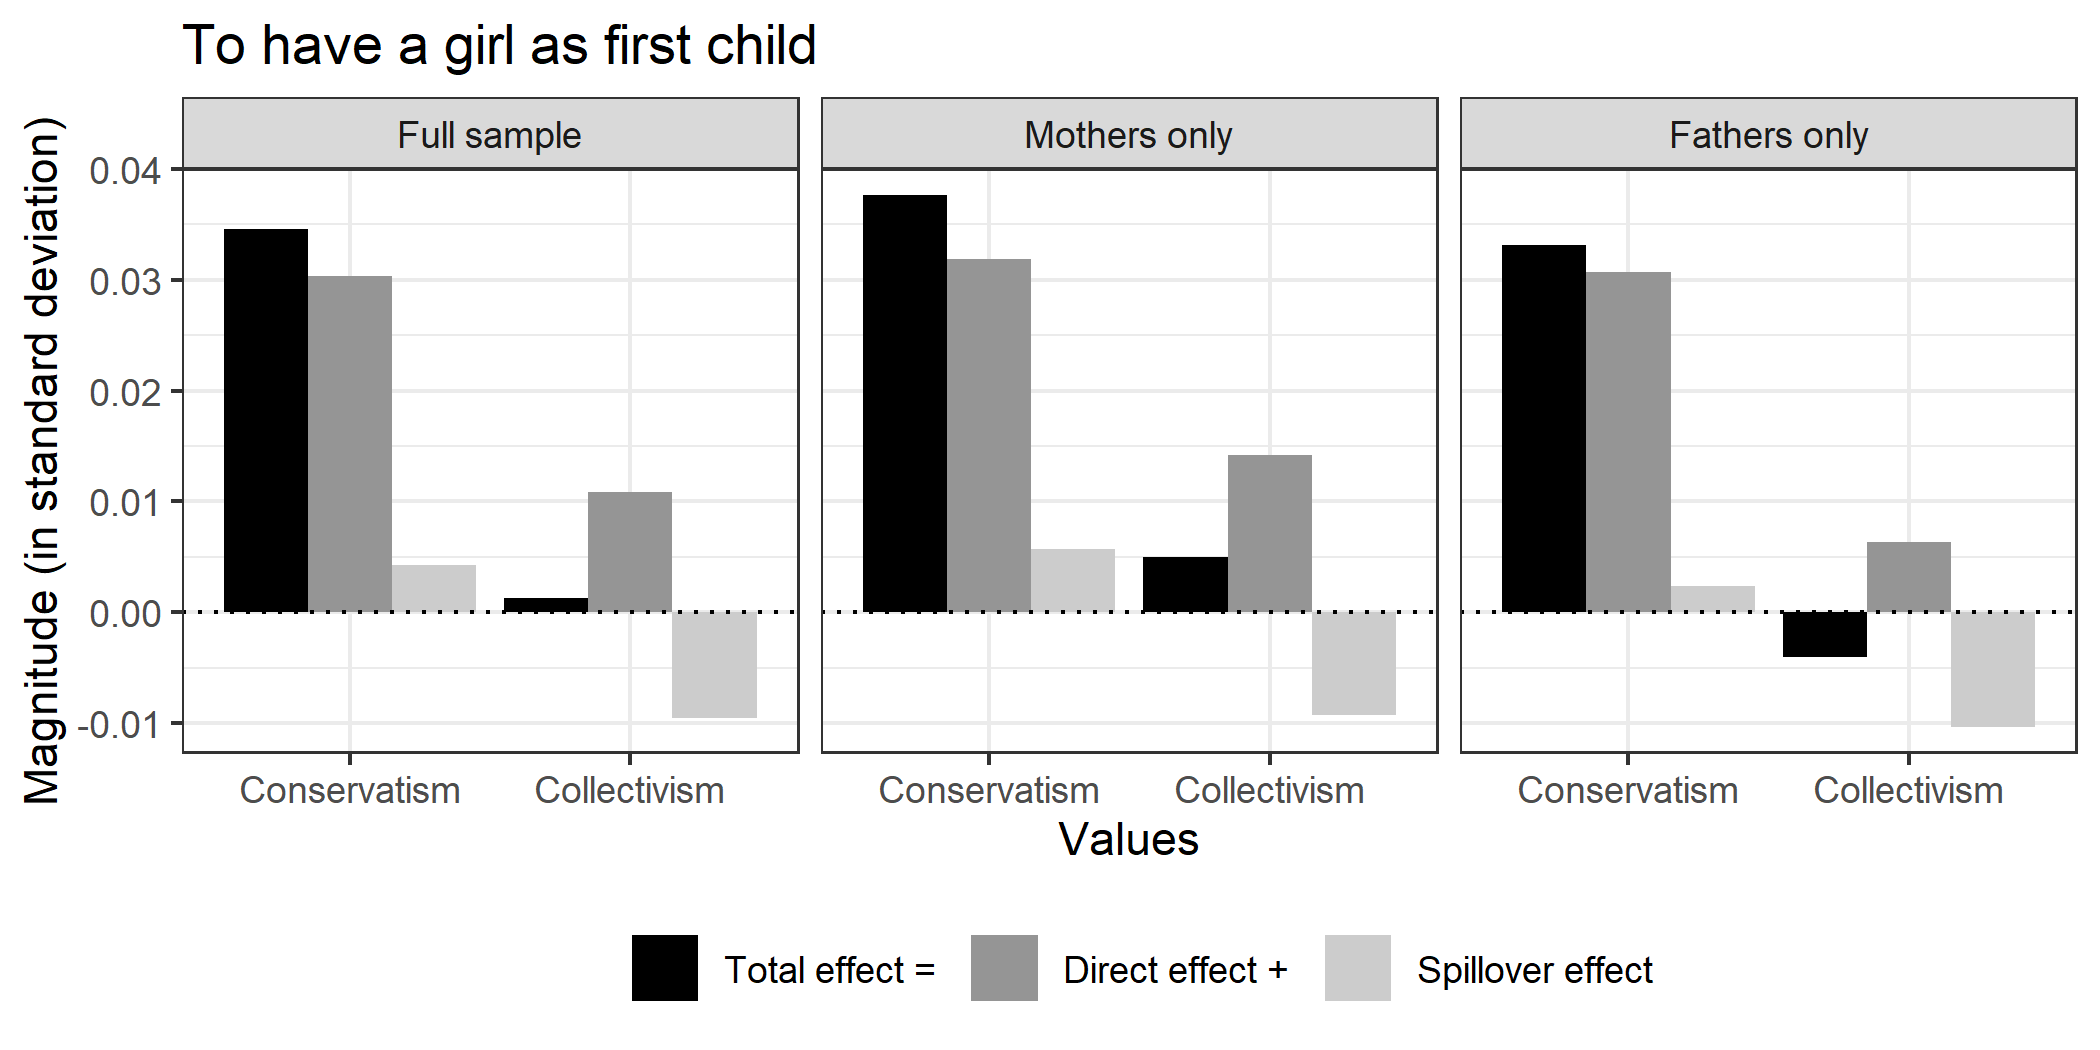
\includegraphics[width=\linewidth]{chap3/graphic/decomp-v5-GFGender.png}
    \hrulefill
	\vspace{-3em}
	\justify\singlespacing\footnotesize{\textit{Notes:} This figure presents the decomposition of the total effect of the girl-first life event on both values, Conservation and Collectivism, according to the parent. The magnitude of each effect is expressed in standard deviation.}
\end{figure}

\begin{figure}[!htb]
    \centering
    \caption{Decomposition of the effect of GirlFirst by education}
    \label{chap3-fig:sem-decomp-v5-GFEduc}
    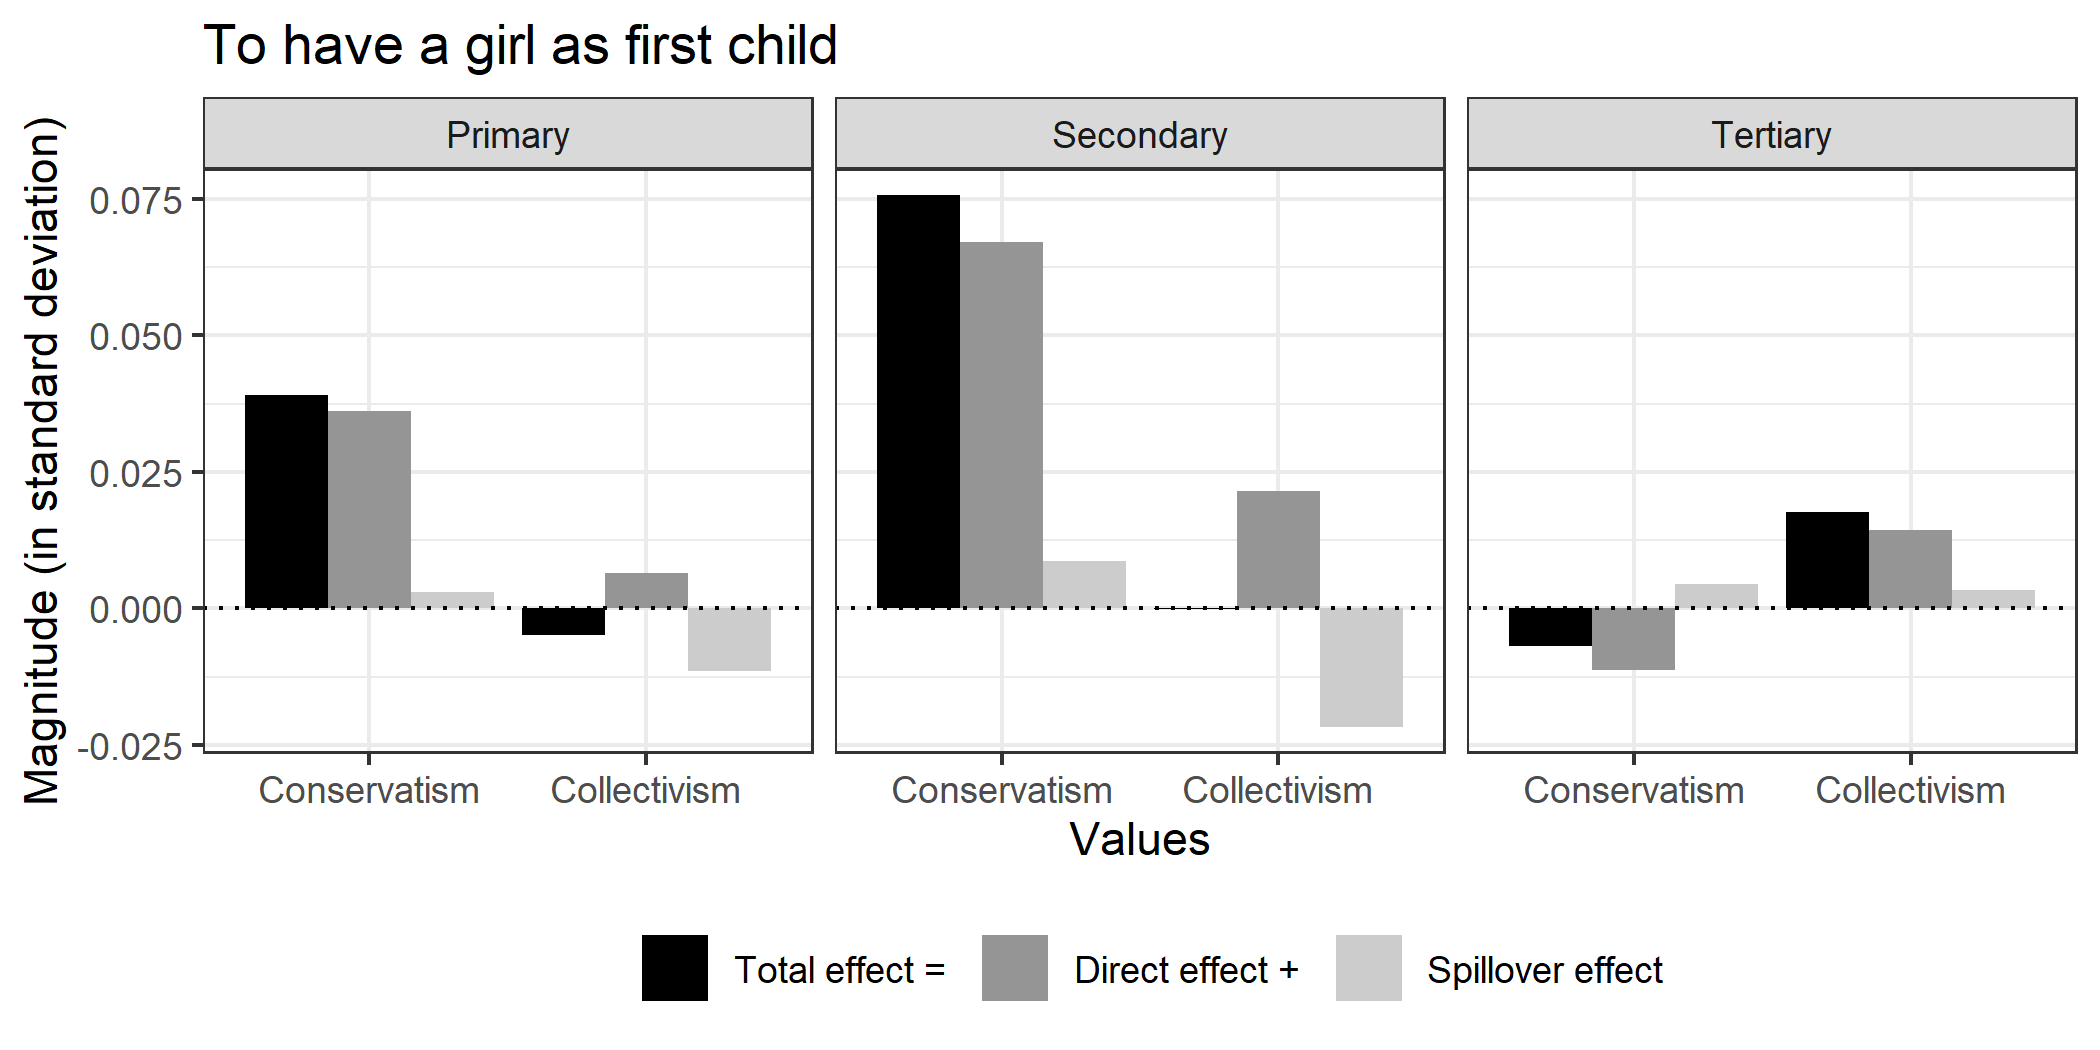
\includegraphics[width=\linewidth]{chap3/graphic/decomp-v5-GFEduc.png}
    \hrulefill
	\vspace{-3em}
	\justify\singlespacing\footnotesize{\textit{Notes:} This figure presents the decomposition of the total effect of the girl-first life event on both values, Conservation and Collectivism, according to education. The magnitude of each effect is expressed in standard deviation.}
\end{figure}

\begin{figure}[!htb]
    \centering
    \caption{Decomposition of the effect of GotCancer with and without the NCDS58 Age 50}
    \label{chap3-fig:sem-decomp-v5-GCNCDS58}
    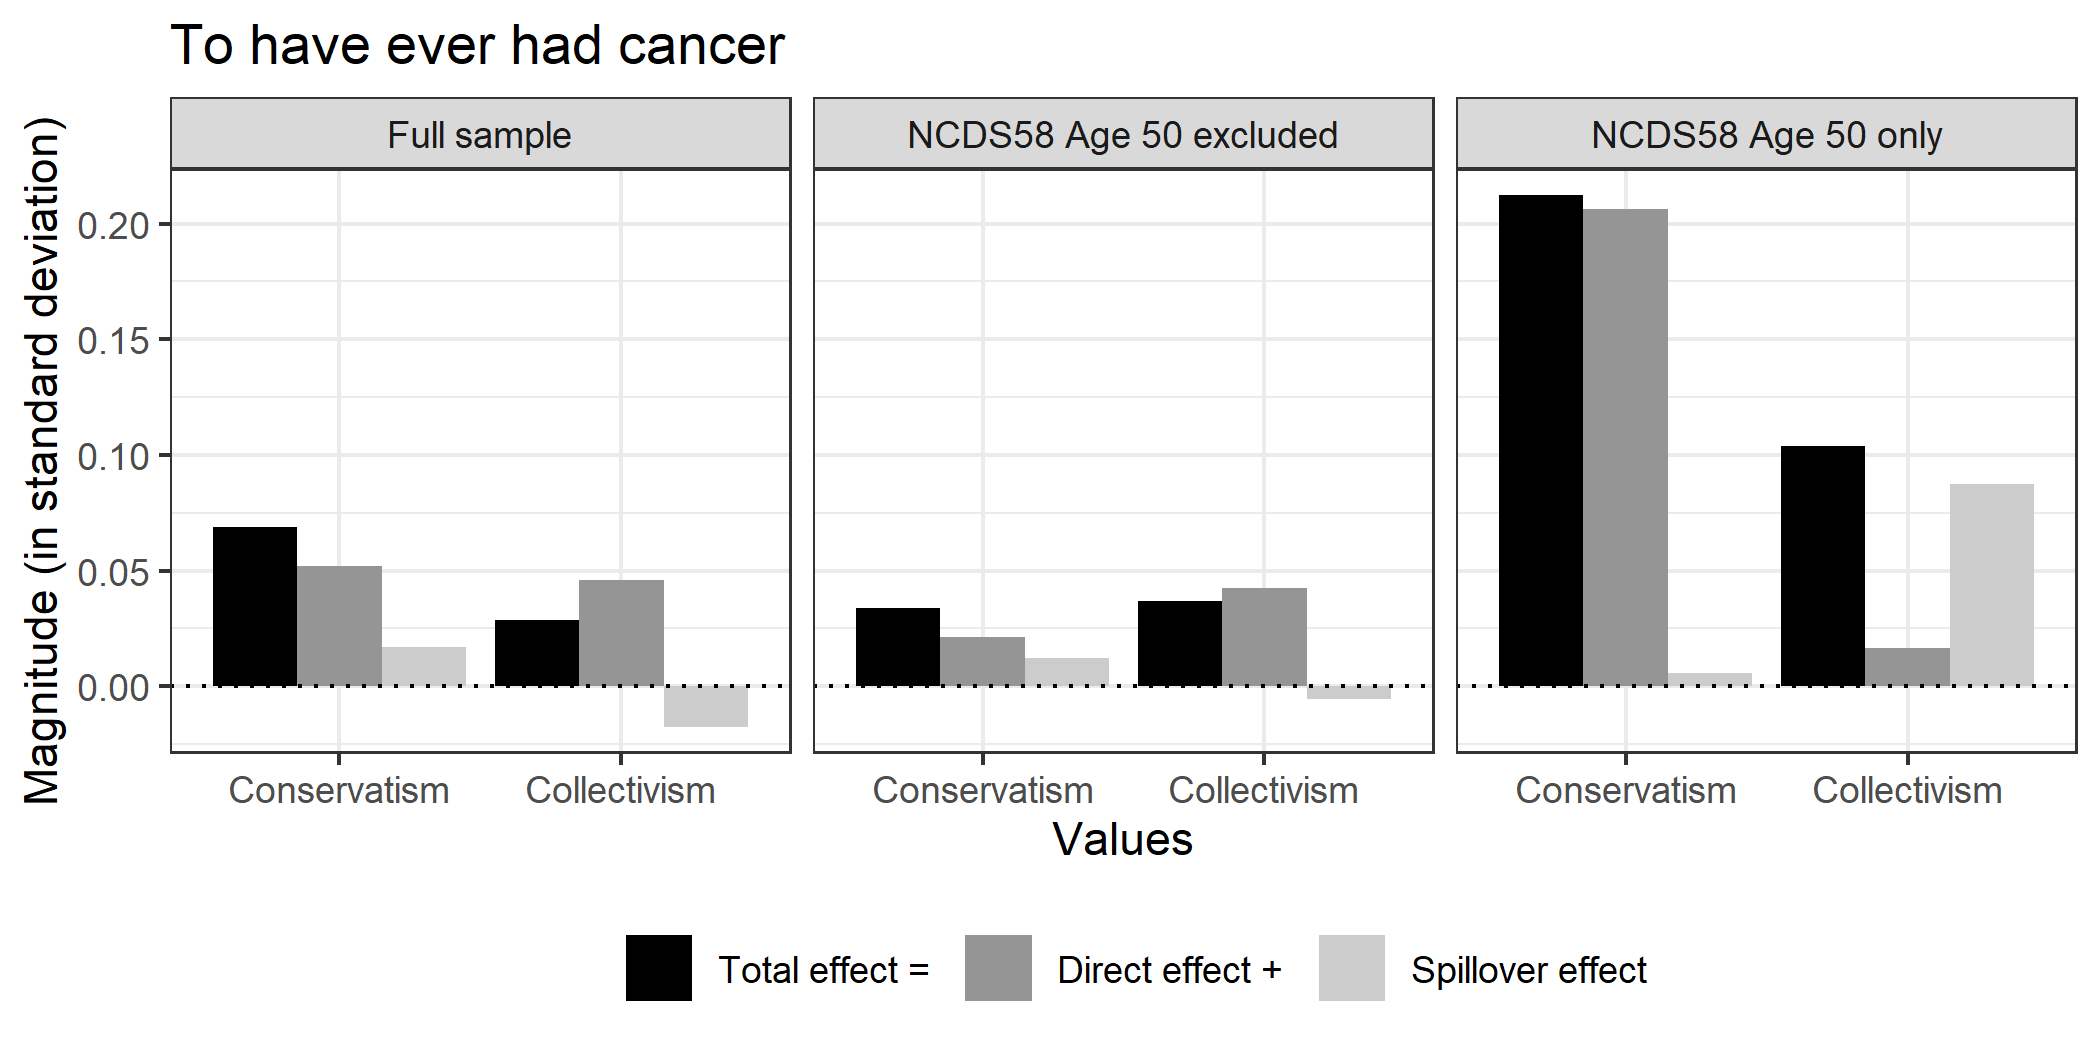
\includegraphics[width=\linewidth]{chap3/graphic/decomp-v5-GCNCDS58.png}
    \hrulefill
	\vspace{-3em}
	\justify\singlespacing\footnotesize{\textit{Notes:} This figure presents the decomposition of the total effect of the got-cancer life event on both values, Conservation and Collectivism, for the NCDS58 cohort at age 50 only and without them. The magnitude of each effect is expressed in standard deviation.}
\end{figure}

\begin{figure}[!htb]
    \centering
    \caption{Decomposition of the effect of GotCancer for those who never have had cancer before}
    \label{chap3-fig:sem-decomp-v5-GCNever}
    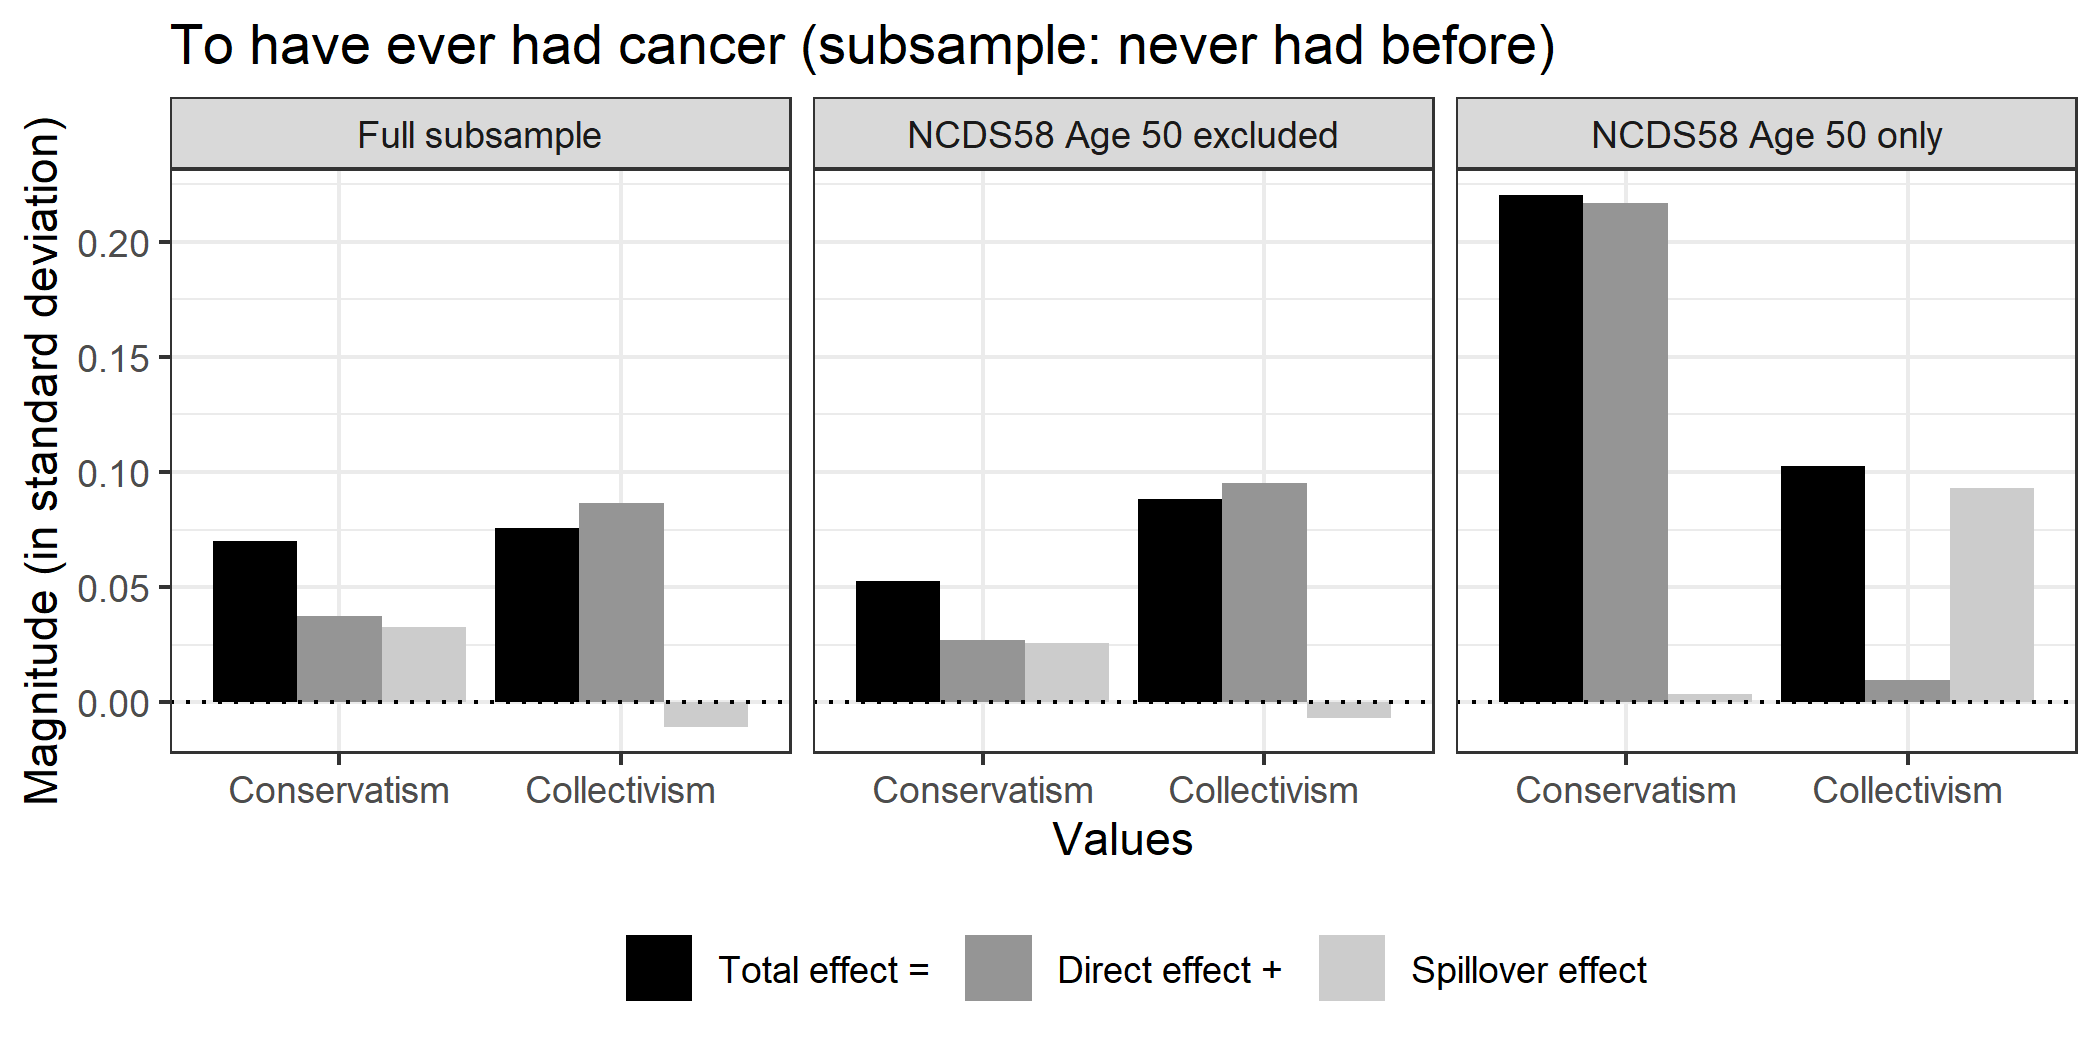
\includegraphics[width=\linewidth]{chap3/graphic/decomp-v5-GCNever.png}
    \hrulefill
	\vspace{-3em}
	\justify\singlespacing\footnotesize{\textit{Notes:} This figure presents the decomposition of the total effect of the got-cancer life event on both values, Conservation and Collectivism, for the NCDS58 cohort at age 50 only and without them. The magnitude of each effect is expressed in standard deviation.}
\end{figure}

\begin{figure}[!htb]
    \centering
    \caption{Decomposition of the effect of BeenUnemp by current activity status}
    \label{chap3-fig:sem-decomp-v5-BUActivity}
    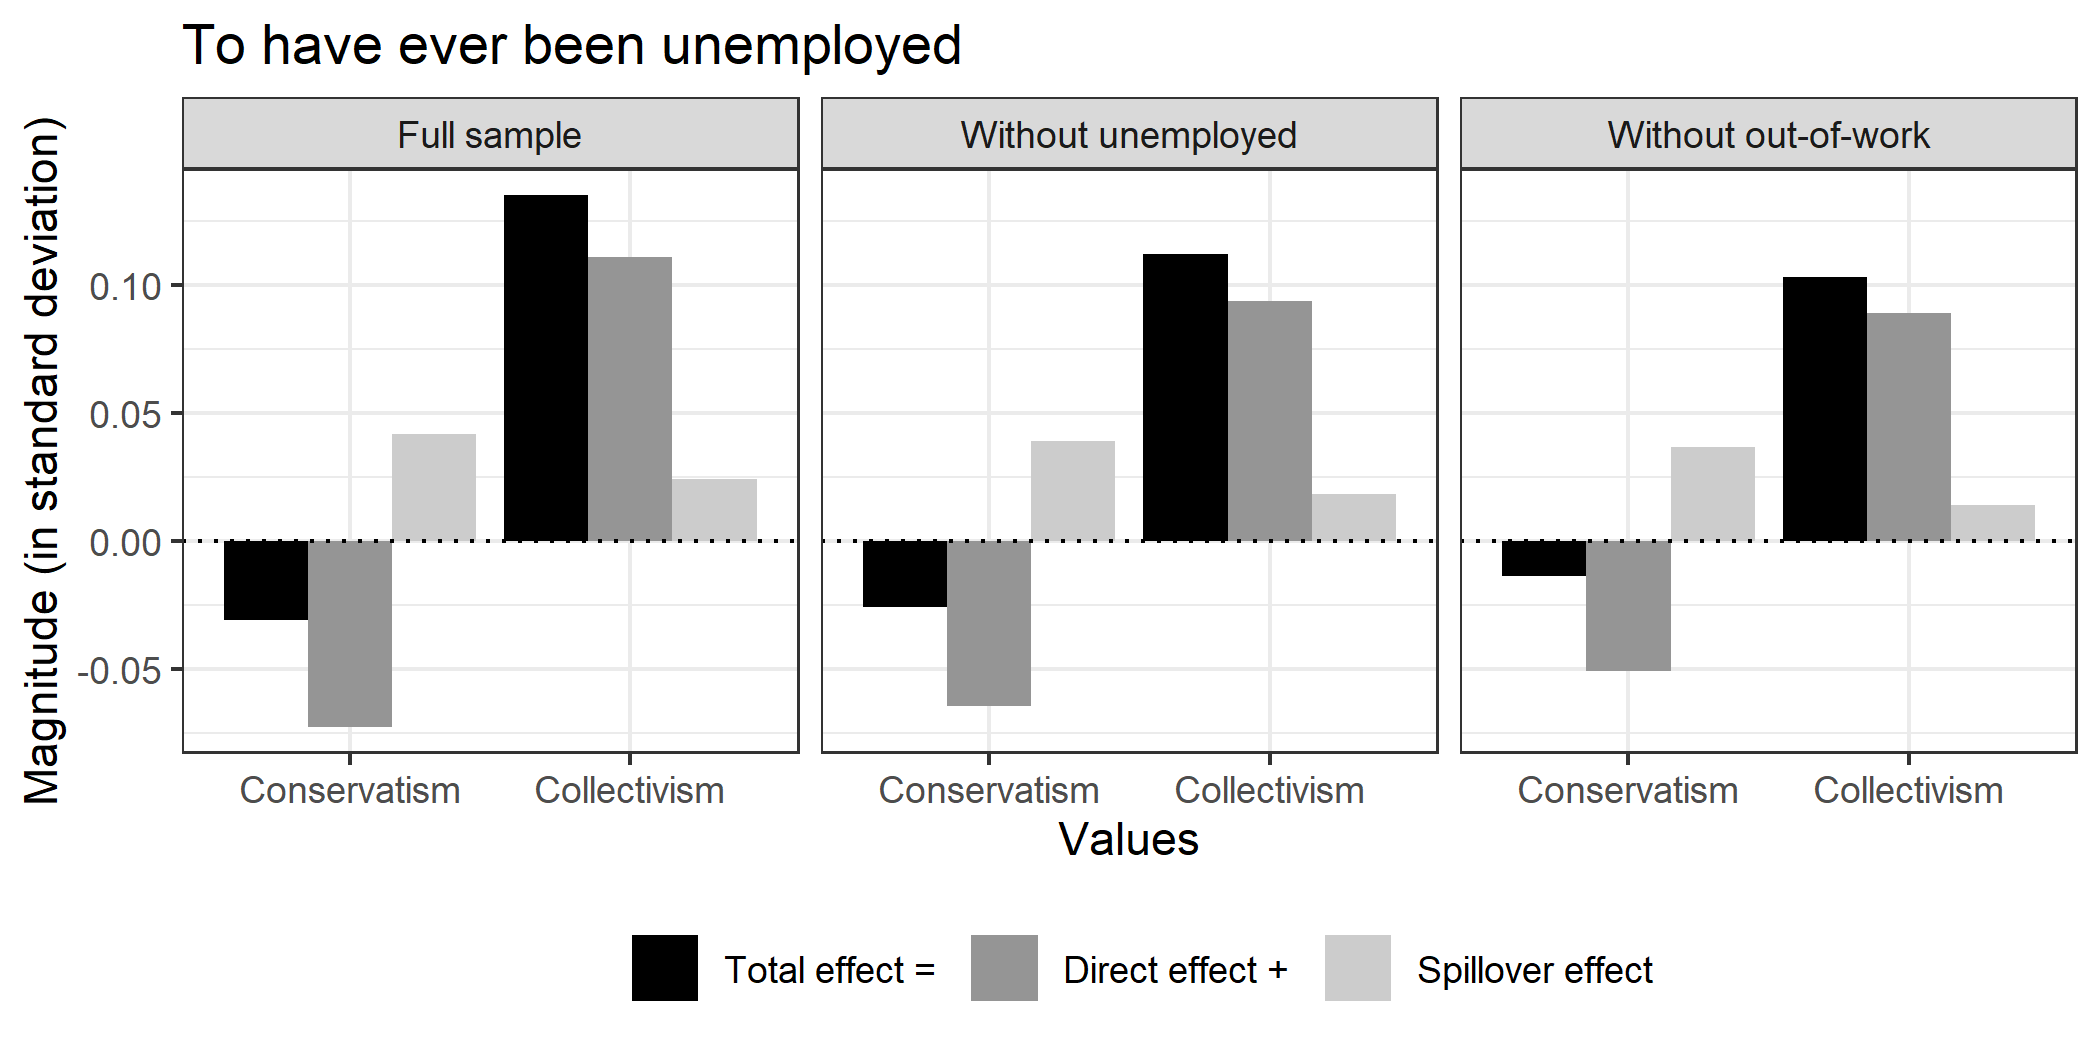
\includegraphics[width=\linewidth]{chap3/graphic/decomp-v5-BUActivity.png}
    \hrulefill
	\vspace{-3em}
	\justify\singlespacing\footnotesize{\textit{Notes:} This figure presents the decomposition of the total effect of the girl-first life event on both values, Conservation and Collectivism, according to the current activity status. The magnitude of each effect is expressed in standard deviation.}
\end{figure}
    \clearpage
    \subsection{Extension of the theoretical framework} \label{chap3-model2}
    To quantify the effect of life events on values, we compare two individuals based on their life trajectories and values. Suppose there exist two individuals $i$ and $j$ that are identical except in their initial value $a_0$, with $a_0^j > a_0^i$. Both individuals belong to the group $\underline{s}$.
Let $\pi_t = \pi(a_t)$ be the probability that a life event occurs which is endogenous to the value $a$.

Suppose the information shock $\Delta a_0$---due to the life event---has the same magnitude for both individuals and would be sufficiently large such that both individuals would identify to the other group. The expected values $a_1$ and $b_1$ for the individual $j$ are
\begin{align}
    \mathbb{E}(a_1^j) &= \frac{\eta_a a^j_0 + \phi_a \underline{a}}{\eta_a+\phi_a} + \pi(a_0^j)\left[ \frac{\eta_a\Delta a_0 + \phi_a(\overline{a}-\underline{a})}{\eta_a+\phi_a} \right],\\
    \mathbb{E}(b_1^j) &= \frac{\eta_b b^j_0 + \phi_b \underline{b}}{\eta_b+\phi_b} + \pi(a_0^j)\frac{\phi_b(\overline{b}-\underline{b})}{\eta_b+\phi_b},
\end{align}
where $\mathbb{E}$ is the expectation operator. It is straightforward to show that these values are symmetrical for the individual $i$. Hence, the biases due to the endogeneity of values can be written as 
\begin{align}
    \mathbb{E}(a_1^j) - a_1^j &= \pi(a_0^j)\times\Delta A,\\
    \mathbb{E}(b_1^j) - b_1^j&= \pi(a_0^j)\times\Delta B,
\end{align}
where $\Delta A \equiv \frac{\eta_a\Delta a_0 + \phi_a(\overline{a}-\underline{a})}{\eta_a+\phi_a}$ is the direct effect of the life changing event on value $a$, and $\Delta B \equiv  \frac{\phi_b(\overline{b}-\underline{b})}{\eta_b+\phi_b}$ is the spillover effect of the life event on value $b$.


Let $\Delta\mathbb{E}v_t$ be the difference in expected value $v_t$ with respect to the true difference between both individuals, namely,
\begin{equation}
    \Delta\mathbb{E}v_t \equiv \mathbb{E}(v_t^j) - \mathbb{E}(v_t^i) - (v_t^j - v_t^i)
\end{equation}
% Suppose both individuals have the same initial values $a_0$. Then, it is straightforward to show that $\Delta\mathbb{E}v_1 = 0$ which means they have the same expected value in period $1$. In our case,
Thus,
\begin{align}
    \Delta\mathbb{E}a_1 &= \left[\pi(a_0^j) - \pi(a_0^i)\right]\times\Delta A,\label{chap3-eq:DeltaA}\\
    \Delta\mathbb{E}b_1 &= \left[\pi(a_0^j) - \pi(a_0^i)\right]\times\Delta B,\label{chap3-eq:DeltaB}
\end{align}
When the probability that the life event occurs is exogenous to values, i.e. $\pi(a_0^j) = \pi(a_0^i)$, there is no bias when estimating the difference between both individuals. 
However, in many cases such as unemployment, this probability is likely to be endogenous, i.e. $\pi(a_0^j) \neq \pi(a_0^i)$, which leads to a bias when gauging the effect of a life event on values.

The magnitude of the bias depends on two components: the difference in terms of probabilities that captures the degree of endogeneity of the life event with respect to values; and the magnitude of either the direct effect or the spillover effect. 
Although the endogeneity issue affects the magnitude of the total effect, it does not change the relative shares of the direct and spillover effects because it is a scale factor of the total effect.

In order to evaluate the magnitude of the bias, I assume that the probability $\pi(a_t)$ is an increasing function of $a_t$. The individual $j$ is more likely to face the life event since $a_0^j > a_0^i$. For simplicity, let assume a binomial logistic function such that
\begin{equation}
    \pi(a_0, \beta_a) = \frac{e^{\beta_a a_0}}{1 + e^{\beta_a a_0}}.
\end{equation}
Note that the intercept has been omitted. Suppose a large endogeneity, namely, that the advantage in terms of the probability that the life event occurs given by a higher value $a$ has an odd-ratio about $2$, which means that an individual with a one-standard-deviation increase in $a_0$ would be two times more likely that the life event occurs. As $\beta_a$ corresponds to the log-odd ratio, it implies that $\beta_a = \log(2)$. 

Table \ref{chap3-tab:gap-a0} summarizes the size of the bias according to the gap in initial values between both individuals.
\begin{table}[!tb]
    \centering
    \caption{Endogeneity bias}
    \label{chap3-tab:gap-a0}
    \begin{threeparttable}
        \setlength{\tabcolsep}{9pt}{}
        \begin{tabular}{lrrrrrrr}
            \toprule 
            & \multicolumn{7}{c}{$\beta_a = \log(2)$} \\
            \cmidrule(lr){2-8}
            $a_0^j$ & -2 & -1 & -0.5 & 0 & 0.5 & 1 & 2\\
            $a_0^i$ & 2 & 1 & 0.5 & 0 & -0.5 & -1 & -2\\
            \midrule
            $\pi(a_0^j)$ & 0.2 & 0.33 & 0.41 & 0.5 & 0.59 & 0.66 & 0.8\\
            $\pi(a_0^i)$ & 0.8 & 0.66 & 0.59 & 0.5 & 0.41 & 0.33 & 0.2\\
            \midrule
            $\Delta\pi$ & -0.6 & -0.33 & -0.17 & 0 & 0.17 & 0.33 & 0.6\\
            \bottomrule
        \end{tabular}
        \begin{tablenotes}[flushleft]
            \footnotesize{\item \textit{Notes}: This table presents the magnitude of the endogeneity bias due to the difference in initial value $a$ between two individuals. $\pi(a_0, \beta_a)$ corresponds to the probability derived from the binomial logistic function and $\Delta\pi$ to the difference in probabilities between both individuals.}
        \end{tablenotes}
    \end{threeparttable}
\end{table}
Since $\lvert \Delta\pi \rvert < 1$, it implies that the endogeneity bias does not change the sign of the direct and indirect effects. 
The (2, -2) and (-2, 2) scenarii are extreme cases in which there is a high degree of polarization in terms of values such that both groups have respectively 2 and -2 standard deviations on average while the average value in the population remains 0. Even in those extreme cases, both the direct and spillover effects can be biased by at the most a scale factor of plus or minus $0.6$.

\end{refsection}